\documentclass{article}
\usepackage{amsmath}
\usepackage{graphicx}

\begin{document}

\title{An Expedition to The Valley of Genomics}
\author{Your Name}
\date{\today}

\maketitle



\section{29-05-2023}
\subsection{Commits}
\paragraph{Commit: bd81b50}
Commit Message: Hoy hicimos un workflow en el que cada commit se va guardado en el diario de laboratorio, con su id y con su mensaje. También se genera una sección de figuras para las figuras que fueron generadas en esa sesión

\paragraph{Commit: 7997396}
Commit Message: pruebo figura

\paragraph{Commit: 50ff4b4}
Commit Message: pruebo figura

\paragraph{Commit: 459b400}
Commit Message: ol

\paragraph{Commit: 1d47914}
Commit Message: prueba

\paragraph{Commit: ba9ba18}
Commit Message: prueba

\paragraph{Commit: 6029931}
Commit Message: prueba

\paragraph{Commit: 2b666e3}
Commit Message: prueba

\paragraph{Commit: b987caa}
Commit Message: prueba

\paragraph{Commit: 39adf1f}
Commit Message: prueba

\paragraph{Commit: 2c3ca23}
Commit Message: prueba

\paragraph{Commit: dcf4e49}
Commit Message: prueba

\paragraph{Commit: fcdee47}
Commit Message: agrego la función parametro para probar las nuevas funciones

\paragraph{Commit: 435d42e}
Commit Message: en linear model lab agrego la capacidad de que la funcion model evaluating y la función calculate gene parameters puedan evaluar las nuevas métricas que se dispongan en la función parametro de phen_gen_weight_functions

\paragraph{Commit: 5b2b424}
Commit Message: agrego en el archivo plots.py la función accuracy para medir individualmente cada métrica

\paragraph{Commit: 99088c5}
Commit Message: modifico especificidad del gen poniendo k en logaritmo

\paragraph{Commit: d558a88}
Commit Message: arreglo la definición que había hecho de especificidad porque estaba mal escrita

\paragraph{Commit: e88a0b3}
Commit Message: prueba cambiando especificidad poniendo a k en un exponente de 10

\paragraph{Commit: cba1811}
Commit Message: arreglo algo que al parecer estaba mal en model_evaluating, que me confundí entre las variables n_metrica y nueva_muetrica, que son, dicho sea de paso, bastante inconvenientes los nombres, debería cambiar por otros

\paragraph{Commit: ff87169}
Commit Message: le saco los argumentos definidos de model evaluating y calculate gene parameters

\paragraph{Commit: 627b278}
Commit Message: ahora cambio True y False de nueva métrica por 'si' 'no', a ver si quizás es algo de eso

\paragraph{Commit: b43bb67}
Commit Message: también agrego una 'a' a un 'n_metric' que faltaba

\paragraph{Commit: 8eb196c}
Commit Message: cambio todos los betha por beta en linear model lab

\paragraph{Commit: 02318c3}
Commit Message: SOLUCIONADO. El problema estaba en calculate_gene_parameters, que asignabamos el booleano a nueva_metrica pero después esa variable cambiaba por el parámetro calculado para el gen candidato, ahora lo solucionamos y debería funcionar todo correctamente

\paragraph{Commit: 49694d7}
Commit Message: es decir que lo anterior no funcionaba no porque no calculase los parámetros sino porque no ordenaba el dataframe

\paragraph{Commit: eef3c10}
Commit Message: al parametro 3 de las nuevas métricas lo corrigo para no tener zerodivisionerror

\paragraph{Commit: e4d8092}
Commit Message: a especificidad_del_gen le agrego la feature type_of_func, para luego probar si queremos exponencial, logarítmica o lineal

\paragraph{Commit: dac3246}
Commit Message: todo funcionando. Las pruebas de métricas nuevas van yendo bien y se están descubriendo cosas interesantes. La especificidad descubrimos que la penalización de k tiene que se logarítmica. Queda por ver la similaridad.

\paragraph{Commit: 09addae}
Commit Message: generé todos los gráficos de rendimiento para especificidad similaridad capitalidad y para algunos a parte. A parte para i y k no corrí porque son complementarios de j, no tendría sentido hacerlo

\paragraph{Commit: d743385}
Commit Message: agrego la función accumulated_accuracy para calcular el accuracy acumulado a lo largo de N y así poder elegir cuantitativamente con cuál métrica me quedo

\paragraph{Commit: 90286d2}
Commit Message: dejo especificidad logarítmica, similaridad logarítmica y capitalid logarítmica, que son las que más accuracy acumulado obtuviewron

\paragraph{Commit: 3a1e9e0}
Commit Message: en este punto están todas las combinaciones algebraicas hechas y también todas las combinaciones de a pares de métricas. Conclusión, la similaridad logarítmica sola es la que mejor desempeña hasta ahora. Agregarle métricaslo mantiene igual

\paragraph{Commit: 3a43cc3}
Commit Message: vuelvo a plotear con los labels y títulos más grandes

\paragraph{Commit: 34e653b}
Commit Message: arreglo los sets reales, recuperando los términos hpo originales, para que sea consistente con las funciones anteriormente escritas, y elimino los anteriores

\paragraph{Commit: 8b6ce8d}
Commit Message: en phen_gen_weight functions agrego la propiedad precision en la función fen_reales_del_gen. Cuando es True, me toma de la base de datos exacta, cuando es False, me toma de la base de datos vaga

\paragraph{Commit: ab6f479}
Commit Message: lo mismo que el anterior commit pero debuuggeado

\paragraph{Commit: eba267b}
Commit Message: creo vage_gene_phenotype_dict.json a partir de phenotype_gene_dict

\paragraph{Commit: bea3b8e}
Commit Message: termino de tunear fen_reales_del_gen. Ya está listo para usarse

\paragraph{Commit: d85db3b}
Commit Message: en plots.py ahora también agrego la evaluación de sets reales y su gráfico

\paragraph{Commit: 60f1b2a}
Commit Message: sesión de pruebas en set reales terminada

\paragraph{Commit: f885698}
Commit Message: hago el plot evaluando en set reales con diferentes métricas

\paragraph{Commit: 41c5e56}
Commit Message: agrego las dos métricas que vamos a usar de ahora en más a model_real_evaluating, el top 50 y la media y mediana de rankings

\paragraph{Commit: 1c731da}
Commit Message: plot de espacio de parametros para j, i y k

\paragraph{Commit: a846b8e}
Commit Message: espacio de parámetros para i j y k normalizadas

\paragraph{Commit: 98d1c1c}
Commit Message: plot para el espacio de parámetros de las comunes i j y k

\paragraph{Commit: 698cfb4}
Commit Message: pesos universales de fenotipos

\paragraph{Commit: 61e4da9}
Commit Message: en la función parámetro ahora le agrego los pesos universales de fenotiupos

\paragraph{Commit: da05a08}
Commit Message: código y .csv con propiedades de los fenotipos como nodos: hijos, ancestros, y frecuencia relativa.

\paragraph{Commit: f1728ed}
Commit Message: calculo para clinvar, bitgenia y gold standard de la profundidad de los fenotipos en la forma de media de nodos hijos y nodos ancestros

\paragraph{Commit: 1dfbf10}
Commit Message: agrego también el cálculo de la media de la frecuencia de aparición de cada fenotipo observado en cada base de datos

\paragraph{Commit: 8609fa5}
Commit Message: agrego owl.py, donde vamos a poder explorar muchos más atributos de fenotipos, enfermedades y genes

\paragraph{Commit: a087ad7}
Commit Message: escribo funciones básicas para obtener genes fenotipos y enfermedades de orpha

\paragraph{Commit: dd0bc73}
Commit Message: termino de escribir las funciones que usan los xml de orpha, ahora también tenemos la clasificación más alta para cada enfermedad

\paragraph{Commit: 797aa68}
Commit Message: gene_phenotype_network antes de ser cambiada a gene_disease_network.py

\paragraph{Commit: ef9d645}
Commit Message: plot de la red de enfermedades

\paragraph{Commit: 84fb6f7}
Commit Message: ploteo de la red de genes en nivel 2

\paragraph{Commit: 5ff862d}
Commit Message: ploteo de la red de diseases de nivel 2

\paragraph{Commit: 3d5531e}
Commit Message: agrego la data de orpha, reestrucuro un poco la carpeta data y también se agrega el .py de redes yt algunos gráficos

\paragraph{Commit: bb902ab}
Commit Message: incorporando orpha y funciones modulares. Todo funcionando a la perfección

\paragraph{Commit: 0c0183e}
Commit Message: casos clínicos corregidos

\paragraph{Commit: f7925a6}
Commit Message: sigo refinando el modelo v2 con orpha

\paragraph{Commit: 4b740da}
Commit Message: agrego la función get_average_age_of_onset() que le damos un orphacode y nos devuelve la edad media de aparición de los síntomas

\paragraph{Commit: 89670d7}
Commit Message: agrego how_many_observed() para la simulación de datos

\paragraph{Commit: 5506a79}
Commit Message: single_disease_simulator funcionando

\paragraph{Commit: 5414c3f}
Commit Message: generating_sets con las primeras pruebas de simulaciones

\paragraph{Commit: 791b3c5}
Commit Message: agregando la feature para que elija los síntomas según una distribución de pesos empíricos

\paragraph{Commit: 702c39f}
Commit Message: en set_simulator_utils, agregamos la distribución de pesos empíricos para cada fenotipo simulado en single_disease_simulator

%CommitsEnd
\subsection{Figures}

\begin{figure}[h] \centering 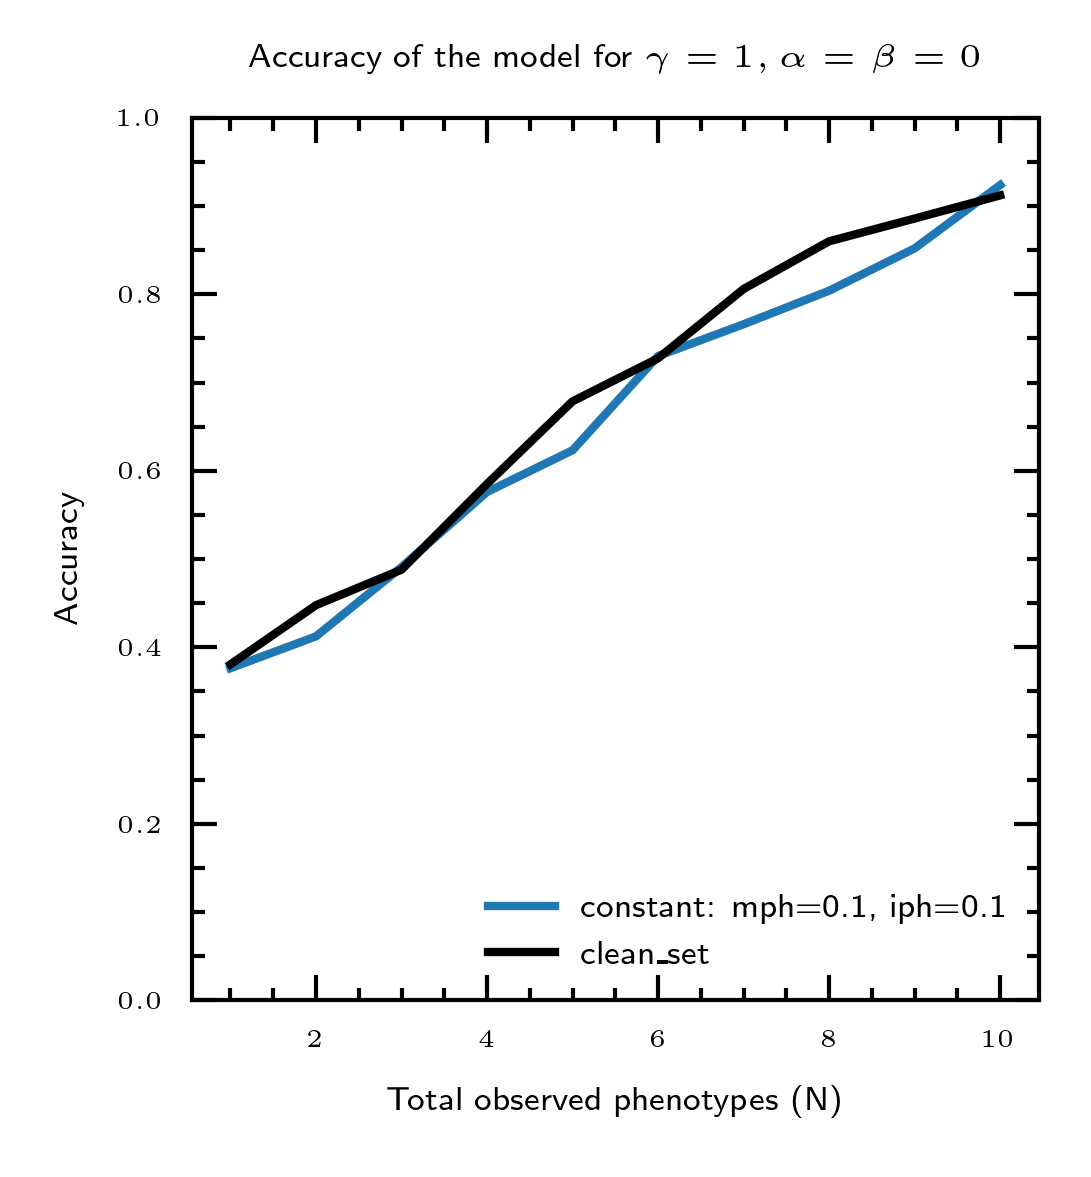
\includegraphics{n.png} \caption{Caption for n.png.} \end{figure}
\begin{figure}[h] \centering 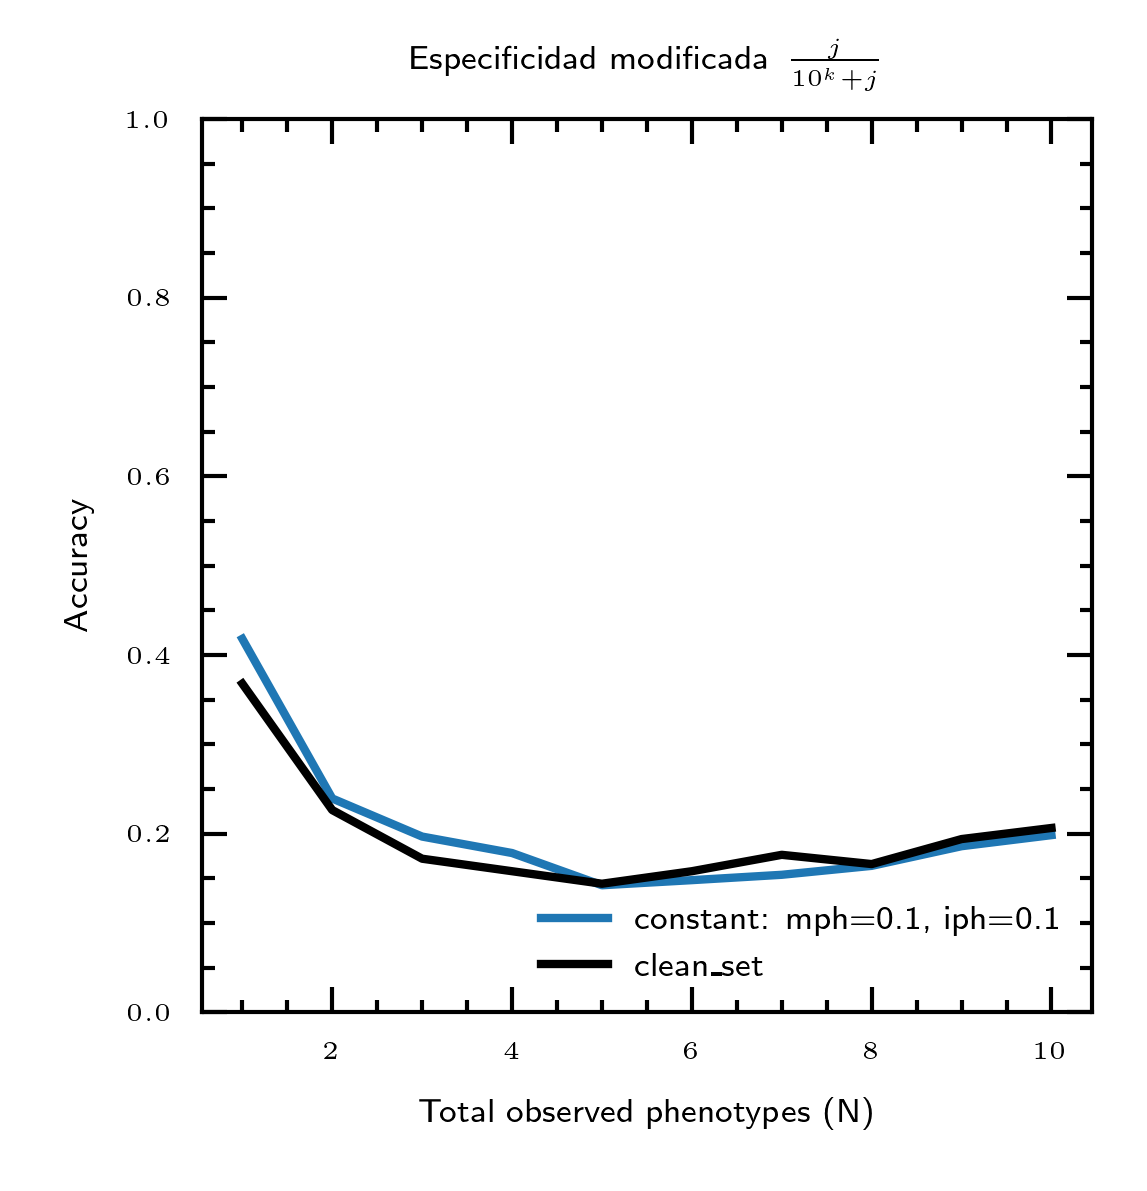
\includegraphics{docs/especificidad_accuracy_exponencial.png} \caption{Caption for docs/especificidad_accuracy_exponencial.png.} \end{figure}
\begin{figure}[h] \centering 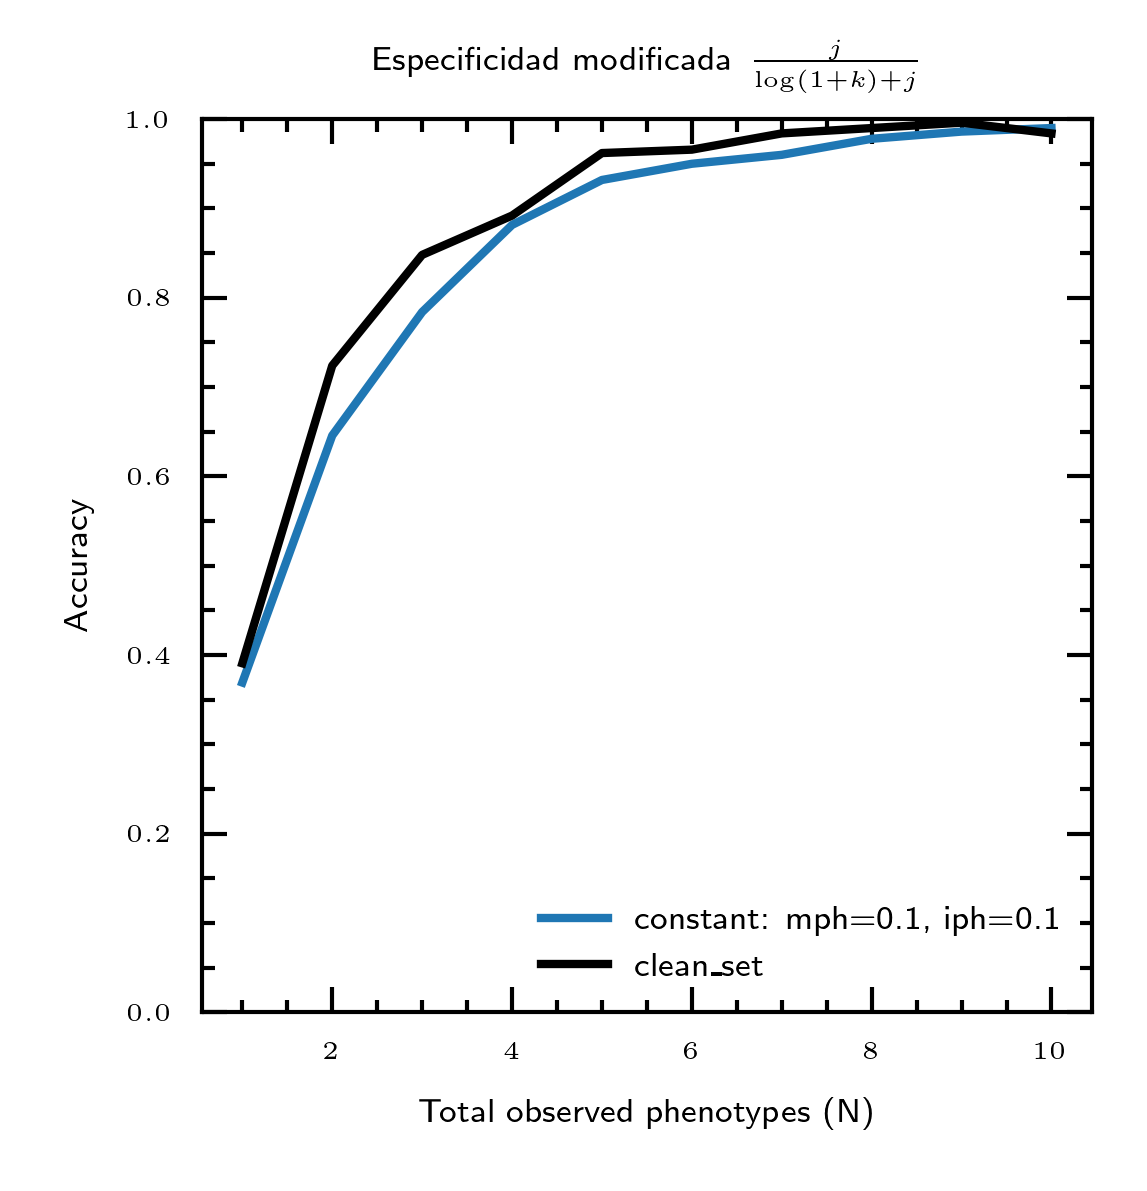
\includegraphics{docs/especificidad_accuracy_logaritmico.png} \caption{Caption for docs/especificidad_accuracy_logaritmico.png.} \end{figure}
\begin{figure}[h] \centering 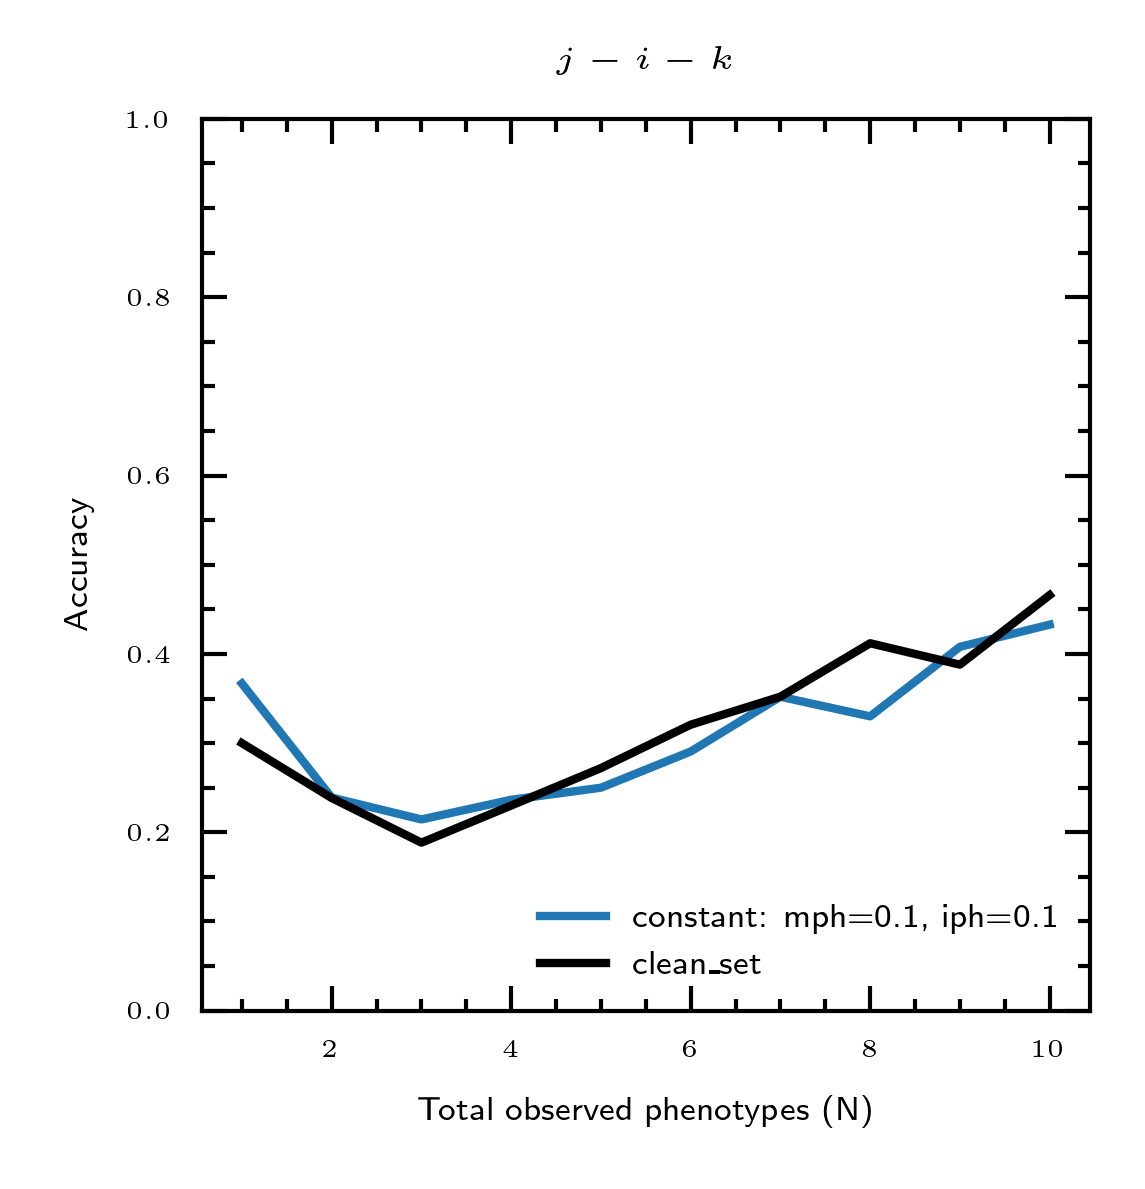
\includegraphics{docs/j-i-k.png} \caption{Caption for docs/j-i-k.png.} \end{figure}
\begin{figure}[h] \centering 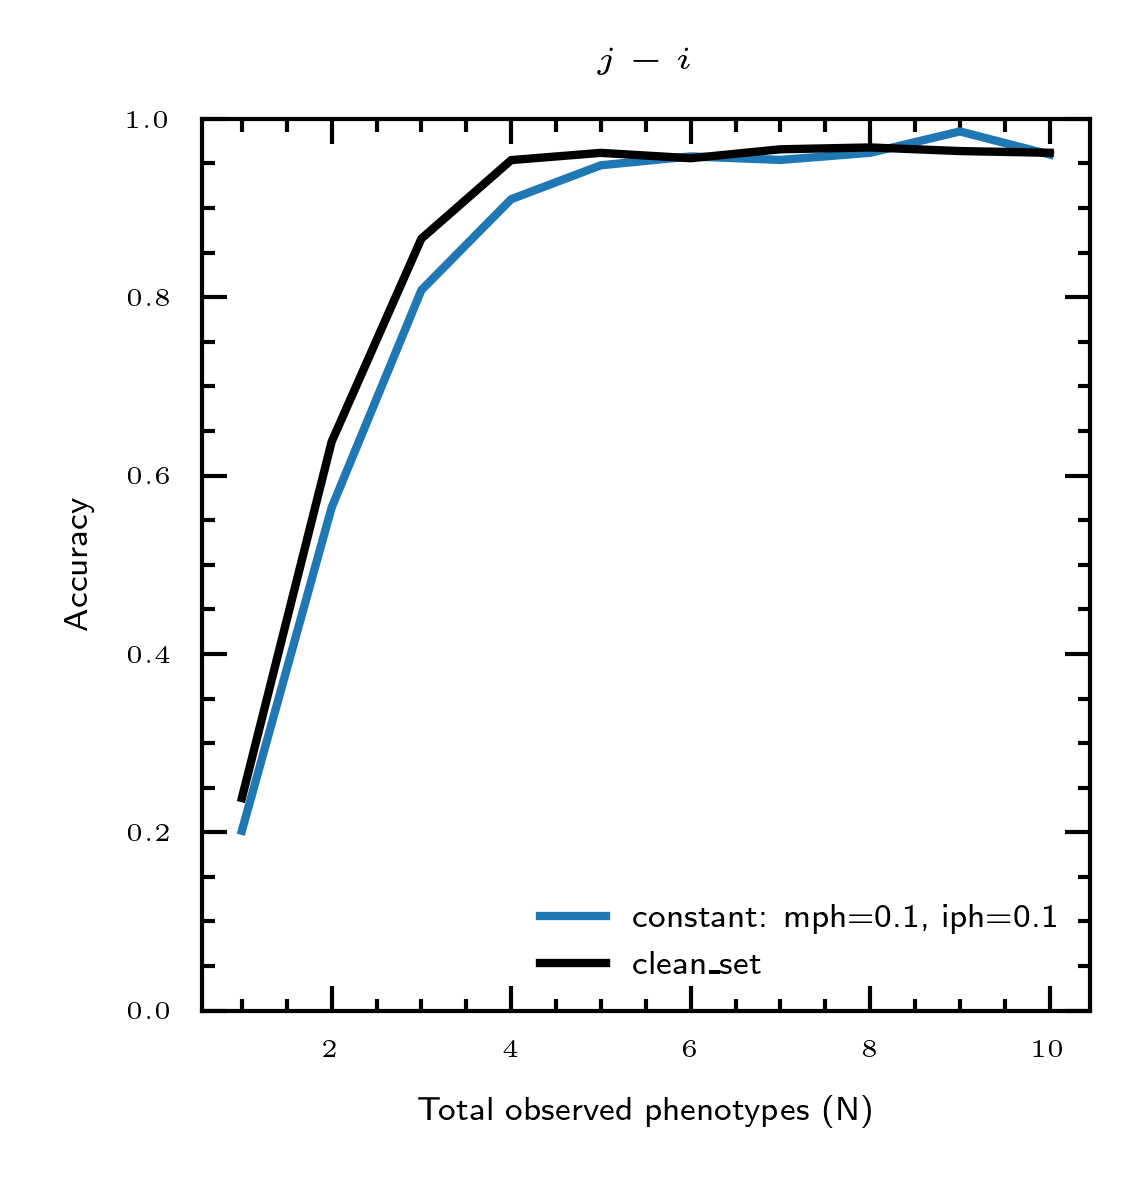
\includegraphics{docs/j-i.png} \caption{Caption for docs/j-i.png.} \end{figure}
\begin{figure}[h] \centering 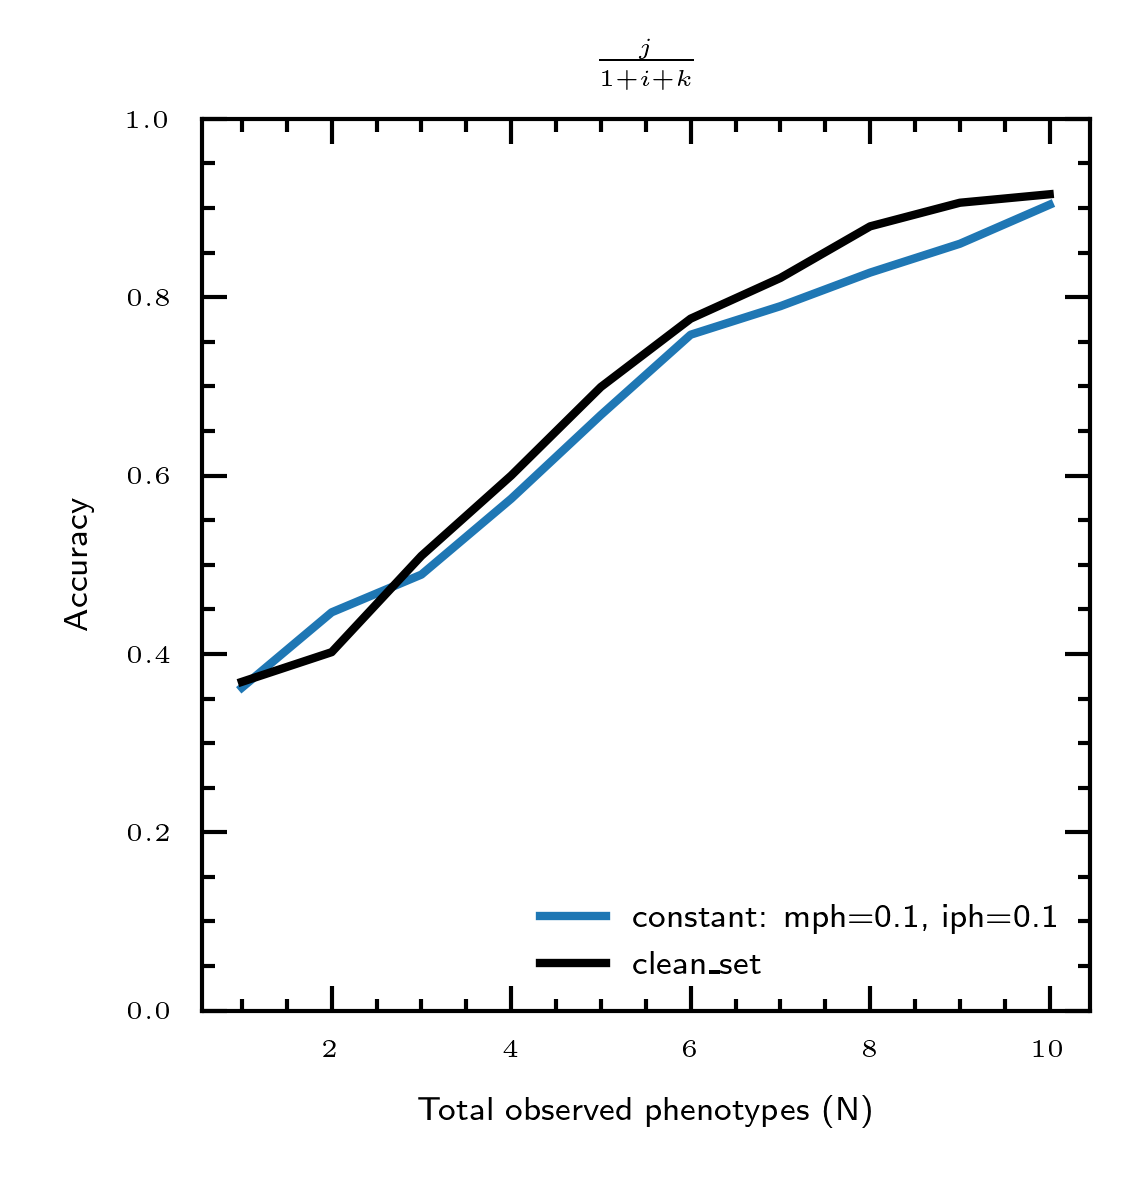
\includegraphics{docs/jsobre1+i+k.png} \caption{Caption for docs/jsobre1+i+k.png.} \end{figure}
\begin{figure}[h] \centering 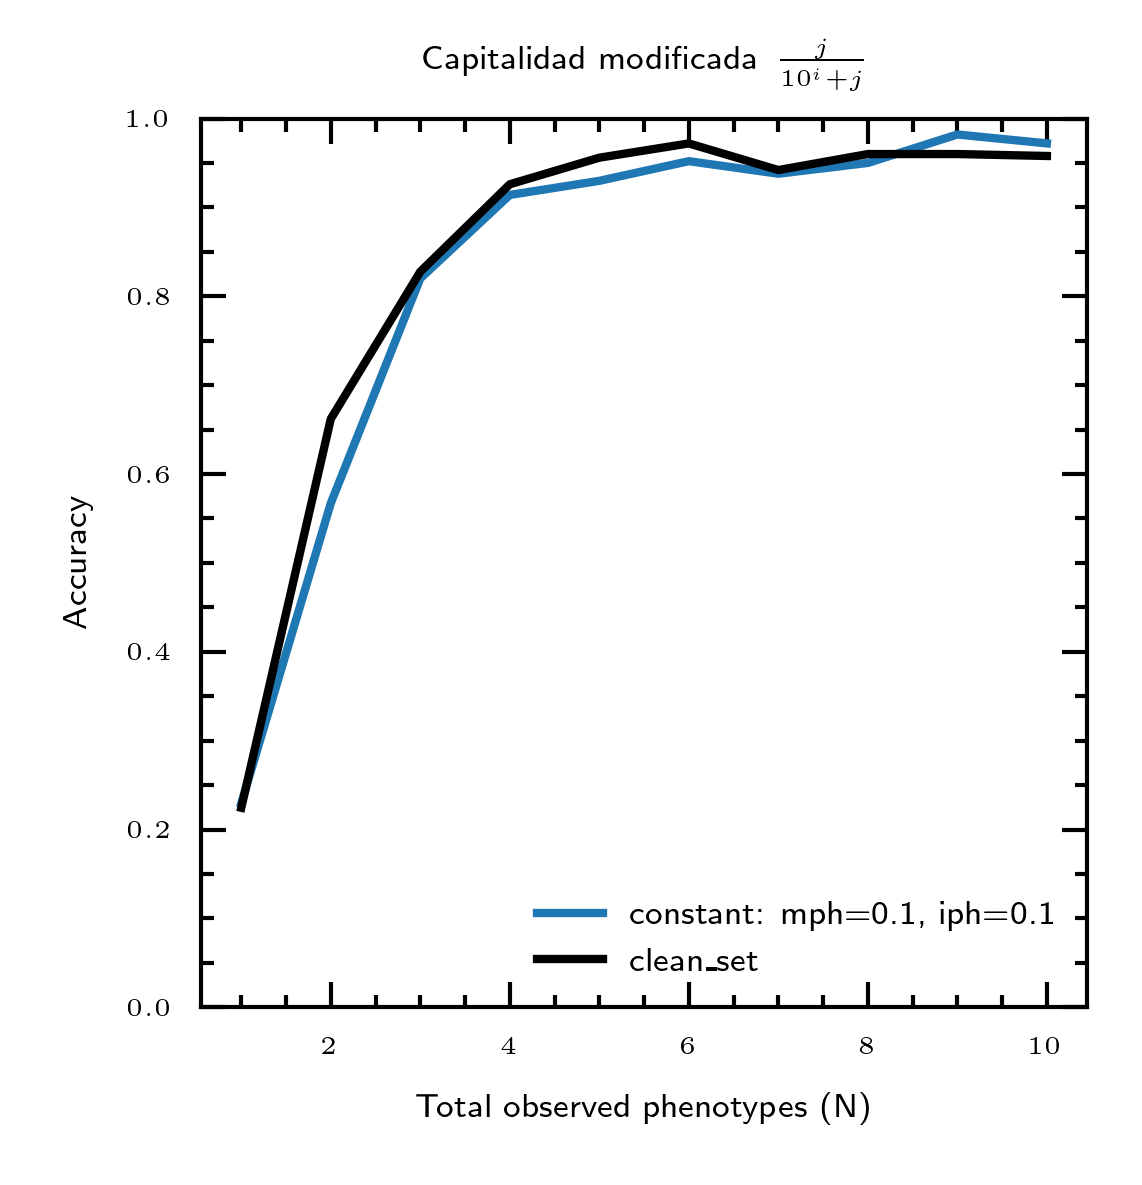
\includegraphics{docs/capitalidad_accuracy_exponencial.png} \caption{Caption for docs/capitalidad_accuracy_exponencial.png.} \end{figure}
\begin{figure}[h] \centering 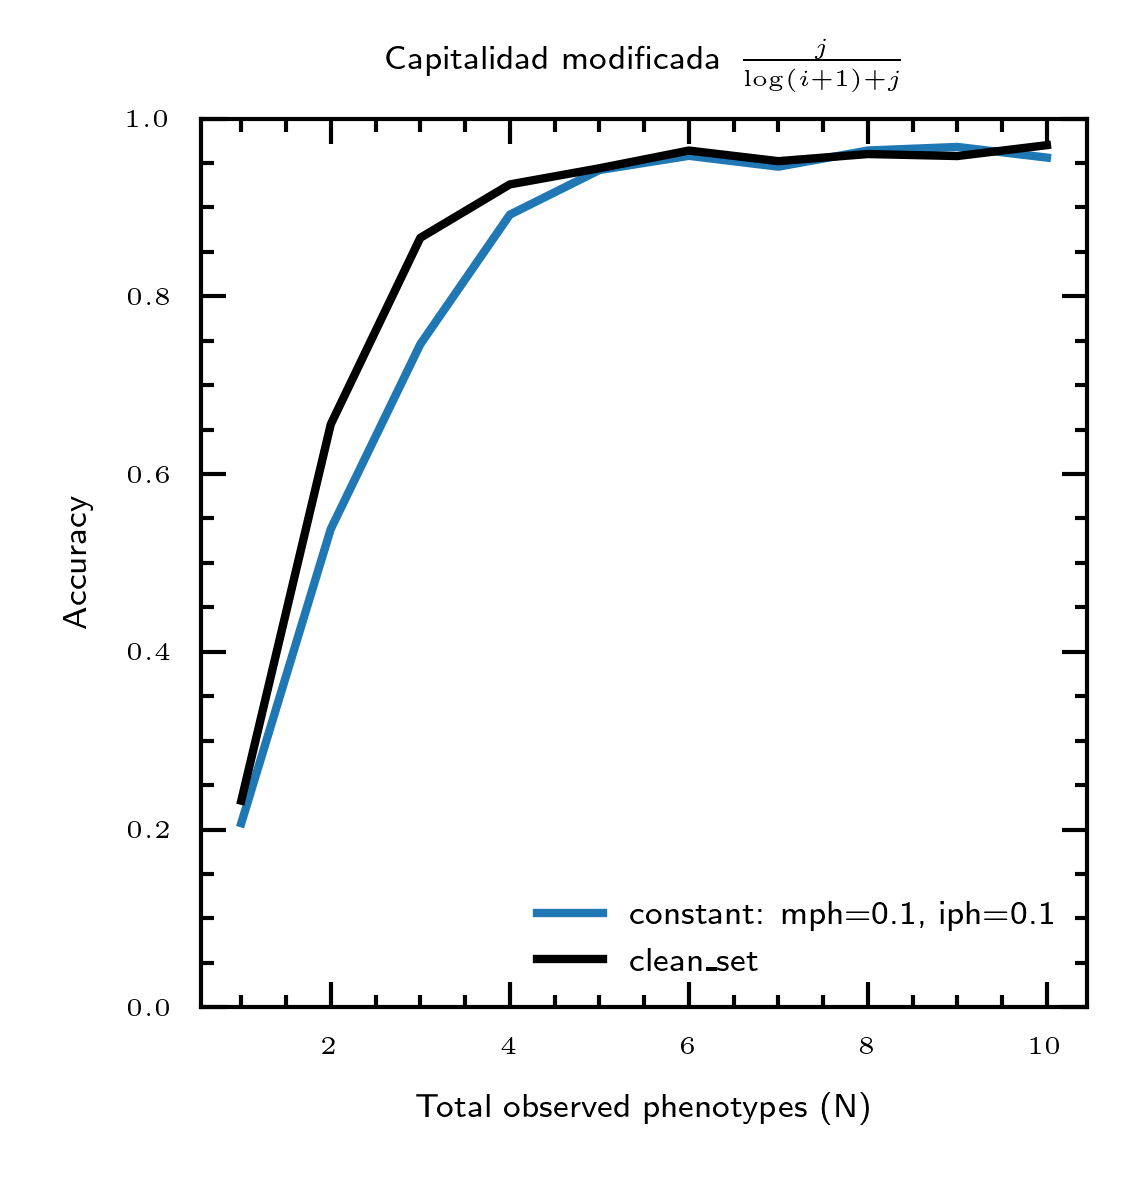
\includegraphics{docs/capitalidad_accuracy_logaritmico.png} \caption{Caption for docs/capitalidad_accuracy_logaritmico.png.} \end{figure}
\begin{figure}[h] \centering 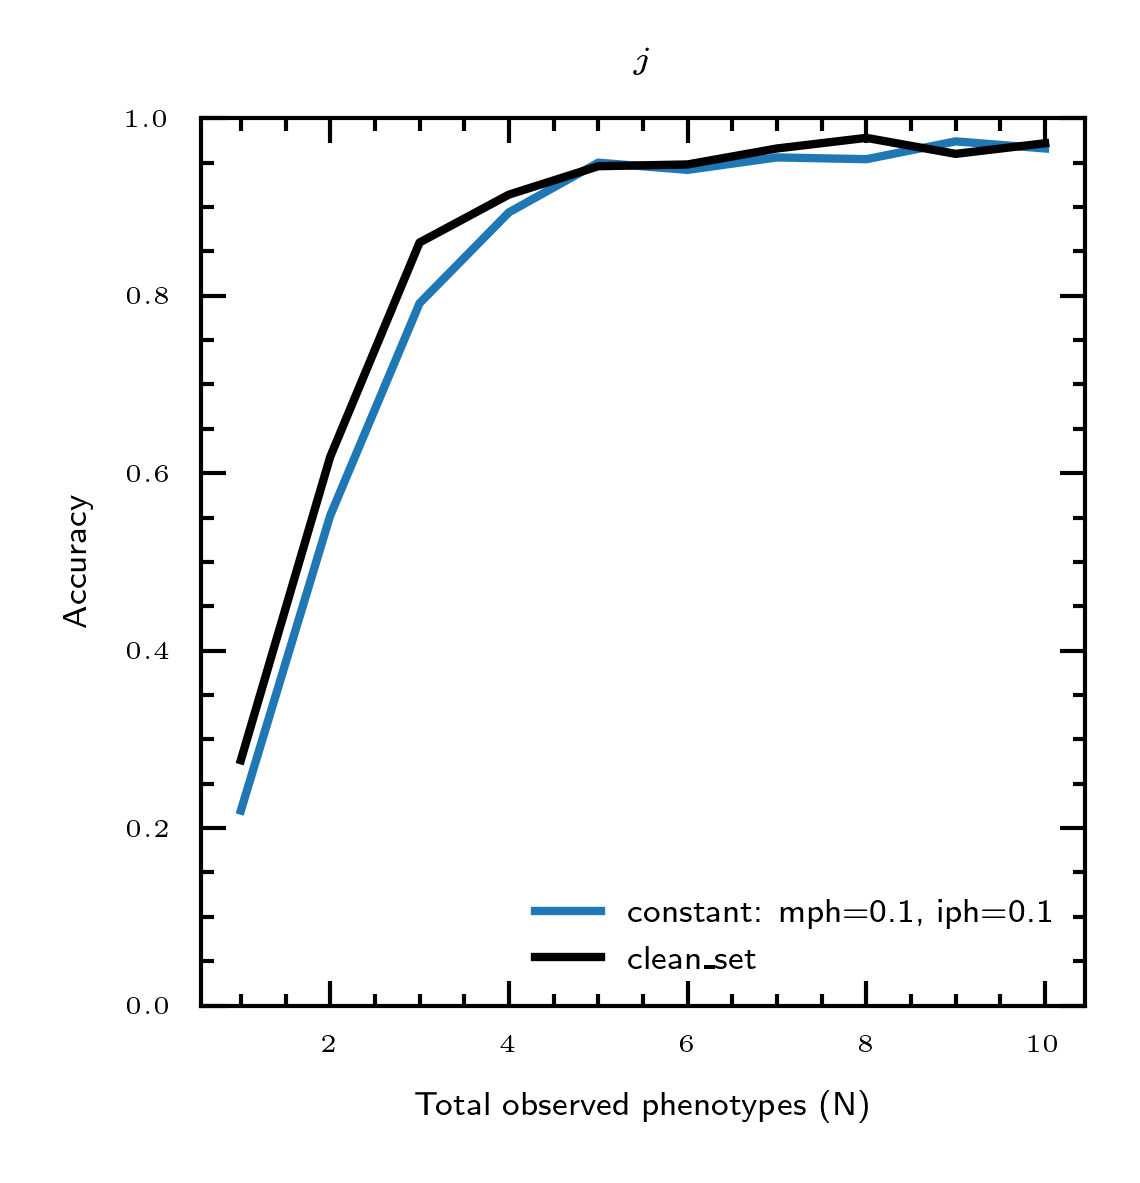
\includegraphics{docs/j_solo.png} \caption{Caption for docs/j_solo.png.} \end{figure}
\begin{figure}[h] \centering 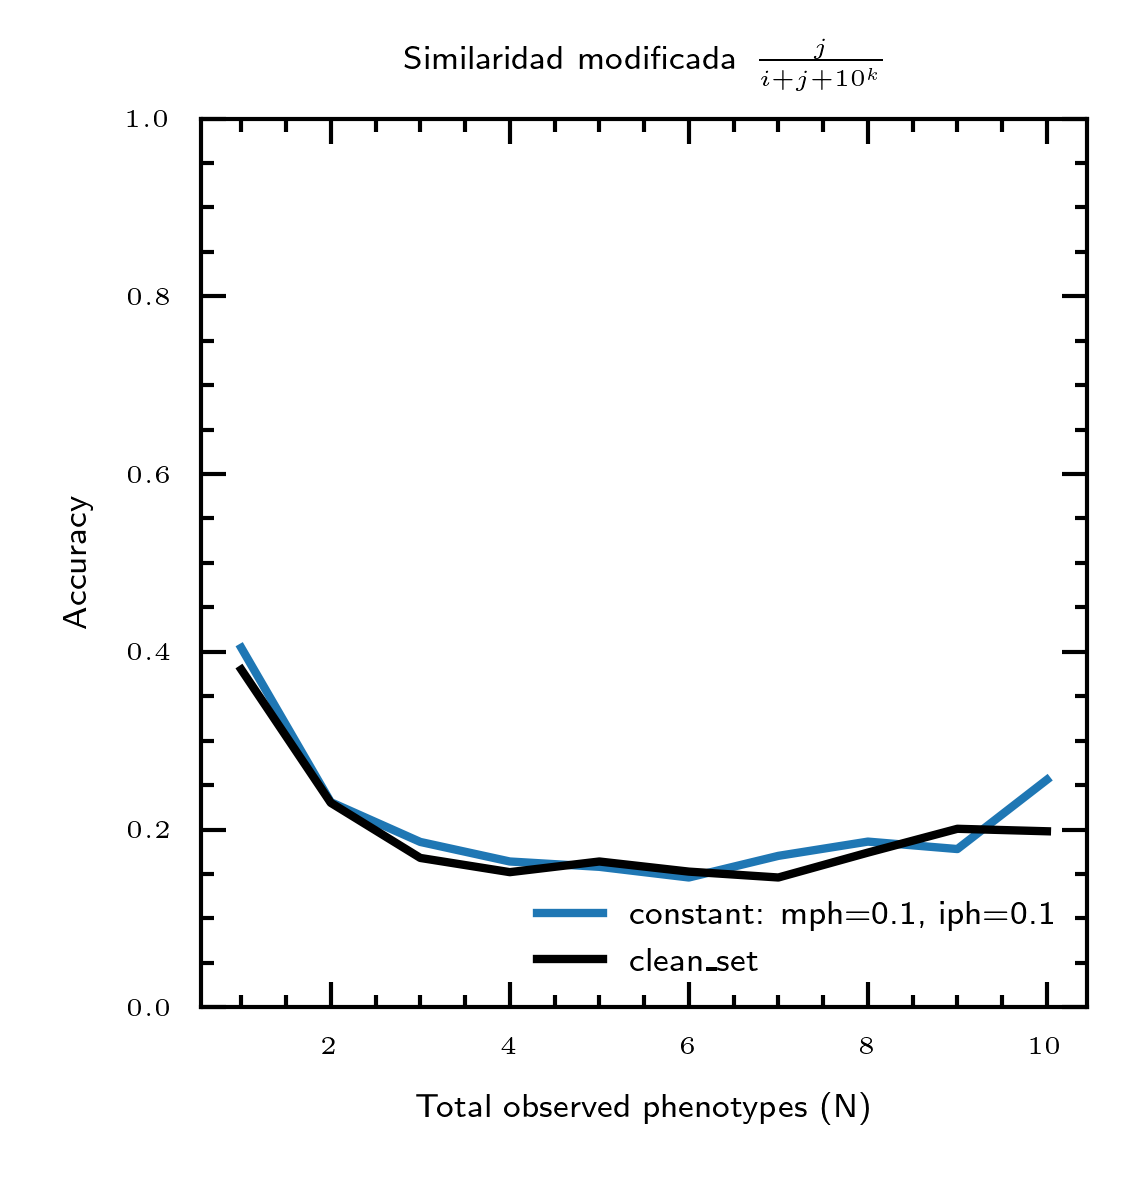
\includegraphics{docs/similaridad_accuracy_exponencial.png} \caption{Caption for docs/similaridad_accuracy_exponencial.png.} \end{figure}
\begin{figure}[h] \centering 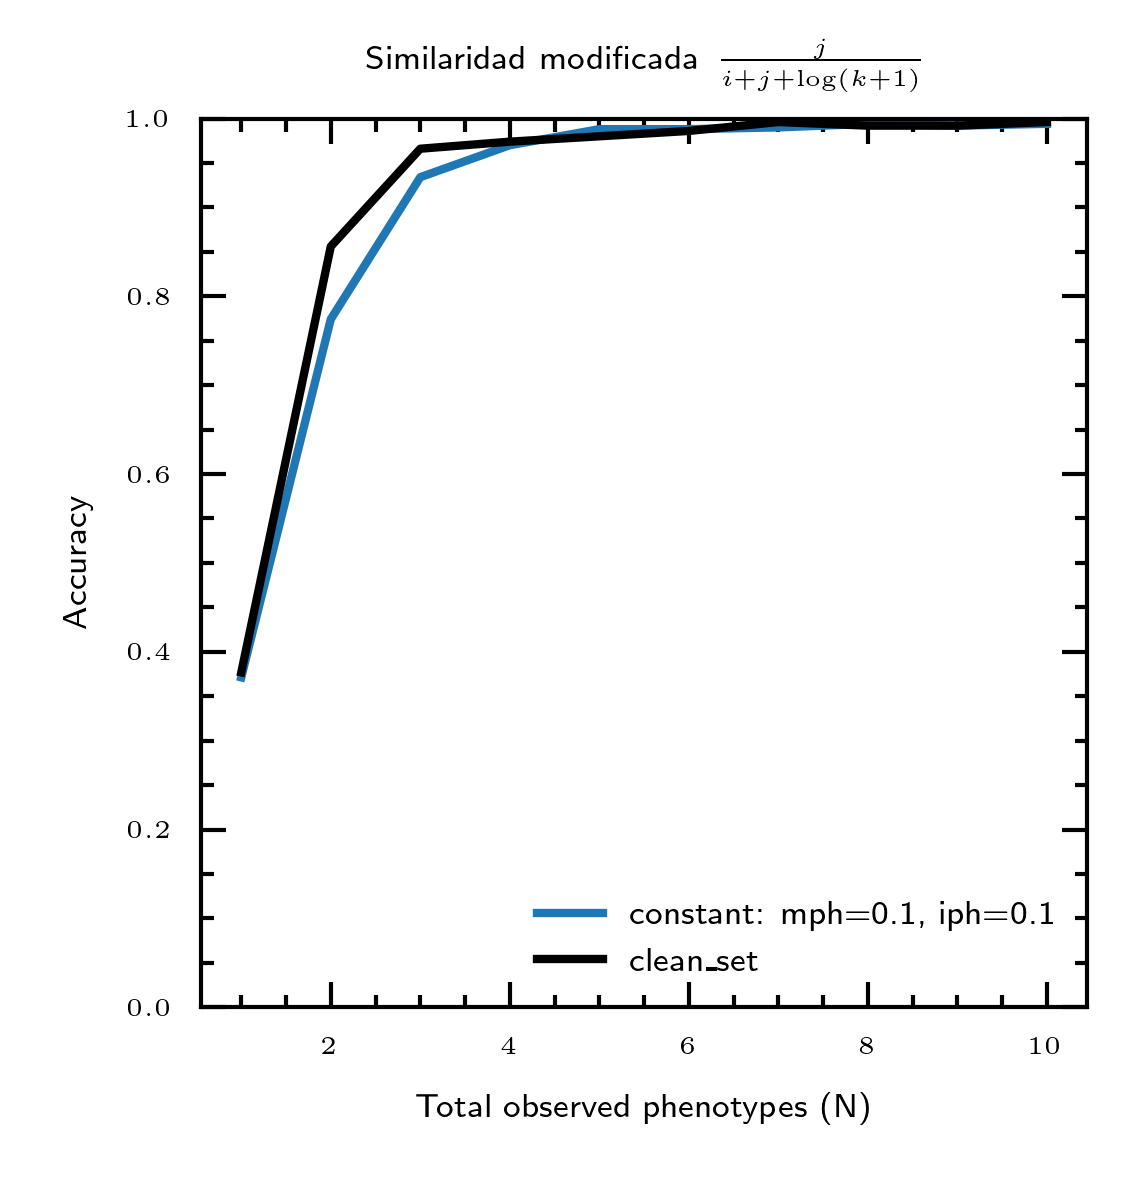
\includegraphics{docs/similaridad_accuracy_logaritmico.png} \caption{Caption for docs/similaridad_accuracy_logaritmico.png.} \end{figure}
\begin{figure}[h] \centering 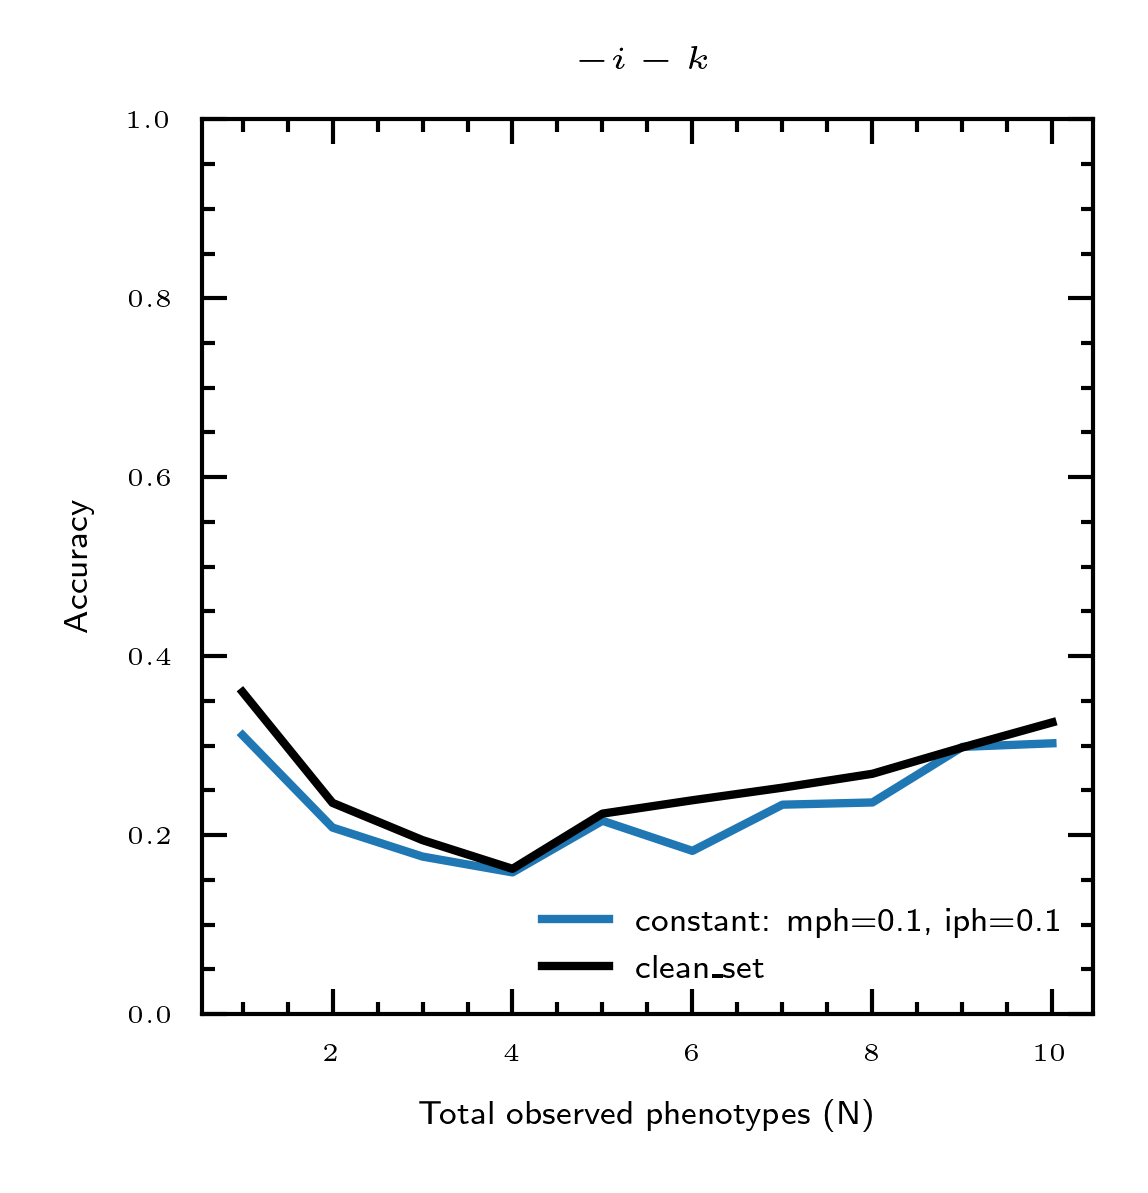
\includegraphics{docs/-i-k.png} \caption{Caption for docs/-i-k.png.} \end{figure}
\begin{figure}[h] \centering 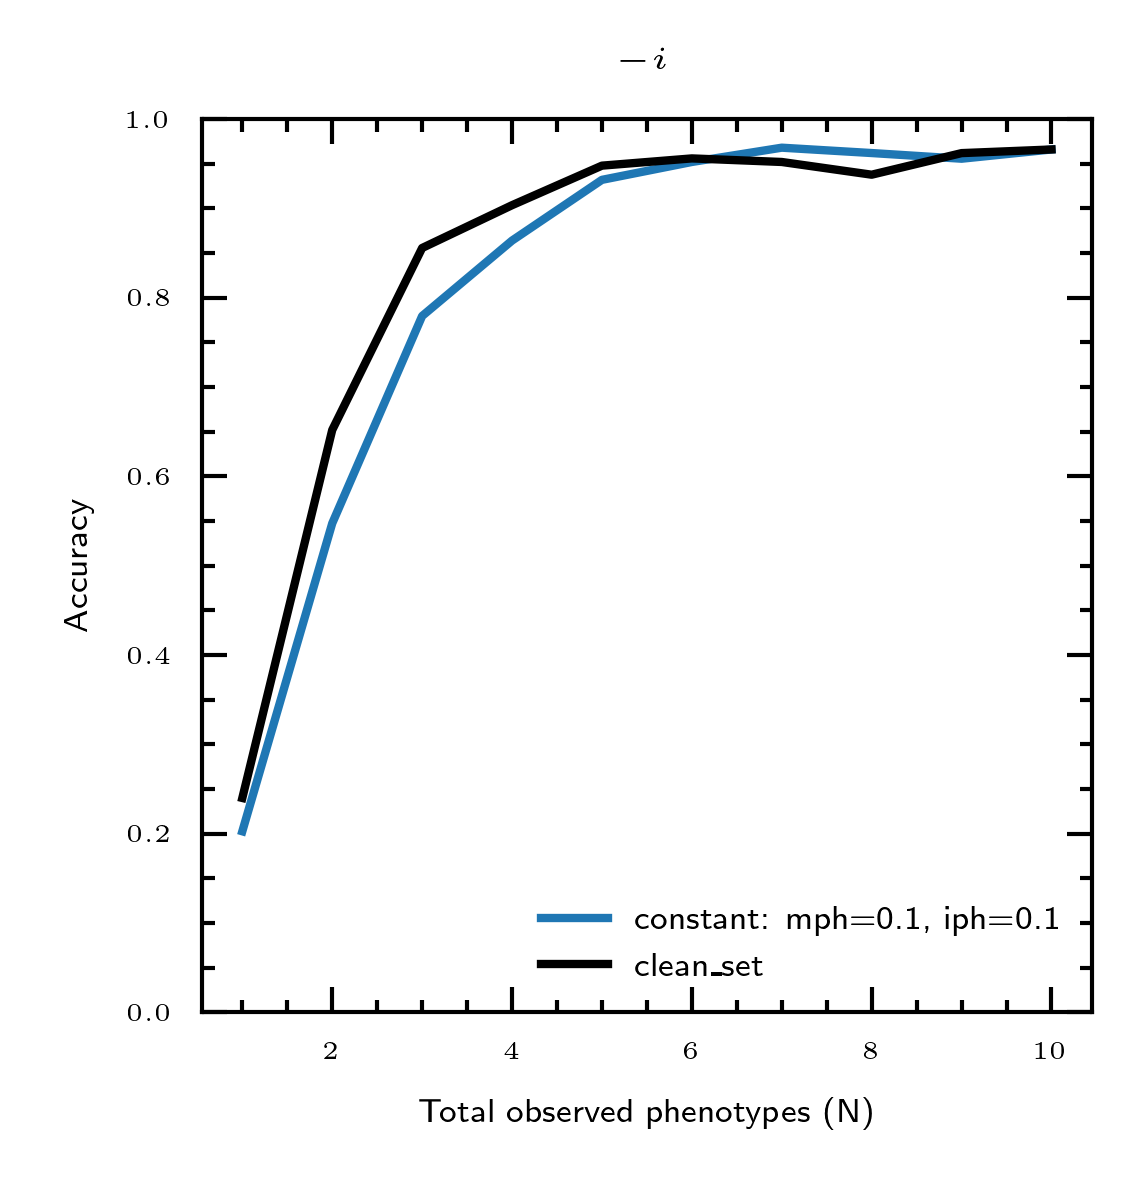
\includegraphics{docs/-i_solo.png} \caption{Caption for docs/-i_solo.png.} \end{figure}
\begin{figure}[h] \centering 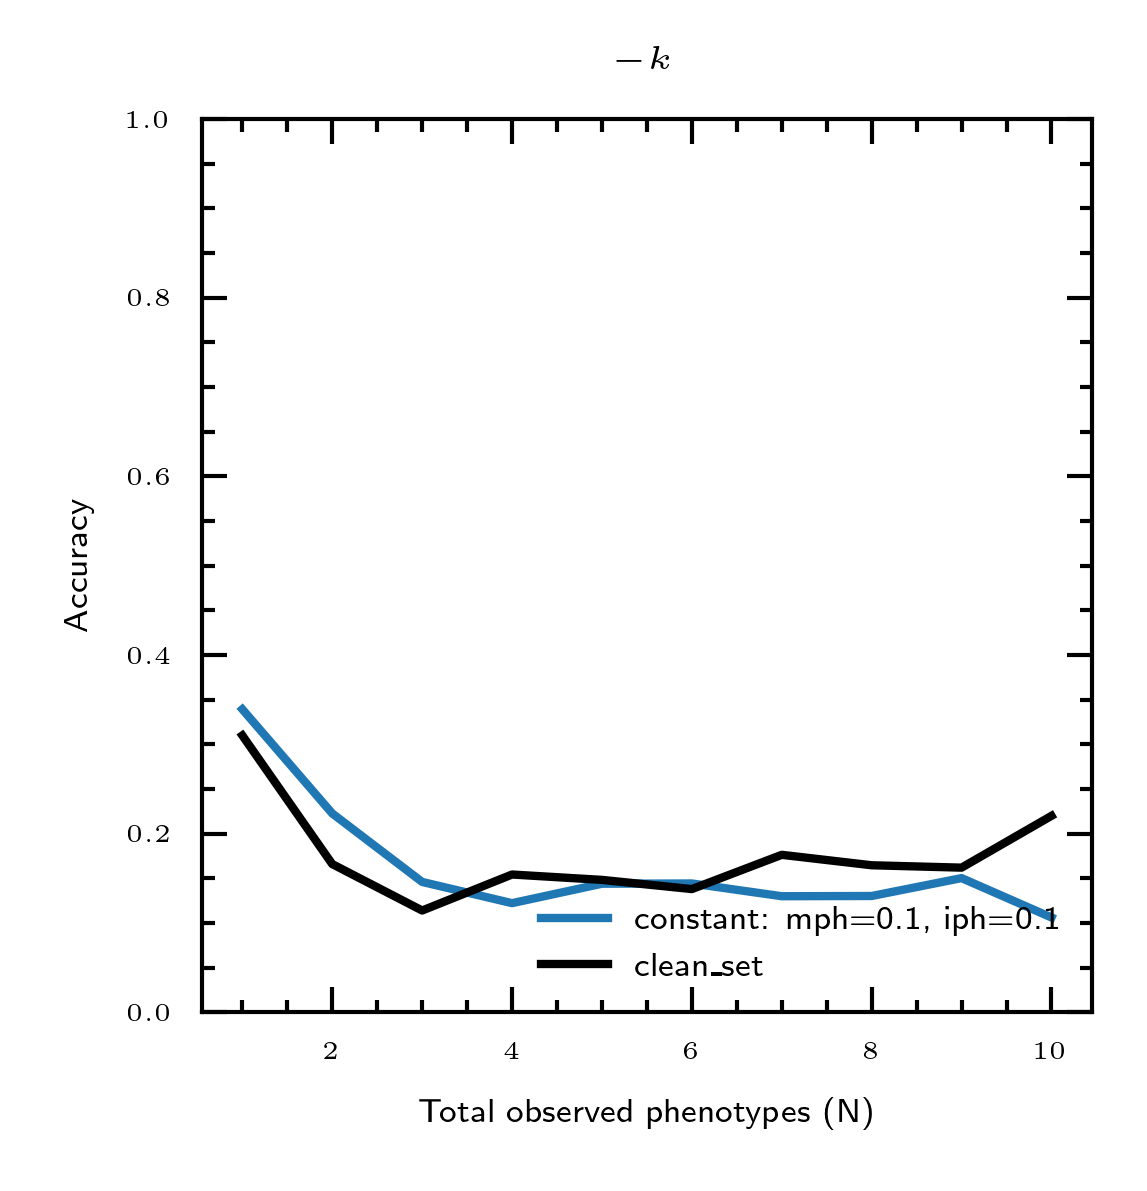
\includegraphics{docs/-k_solo.png} \caption{Caption for docs/-k_solo.png.} \end{figure}
\begin{figure}[h] \centering \includegraphics{docs/cap_mas_esp_mas_sim.png} \caption{Caption for docs/cap_mas_esp_mas_sim.png.} \end{figure}
\begin{figure}[h] \centering \includegraphics{docs/cap_mas_sim.png} \caption{Caption for docs/cap_mas_sim.png.} \end{figure}
\begin{figure}[h] \centering \includegraphics{docs/esp_mas_cap.png} \caption{Caption for docs/esp_mas_cap.png.} \end{figure}
\begin{figure}[h] \centering \includegraphics{docs/esp_mas_sim.png} \caption{Caption for docs/esp_mas_sim.png.} \end{figure}
\begin{figure}[h] \centering 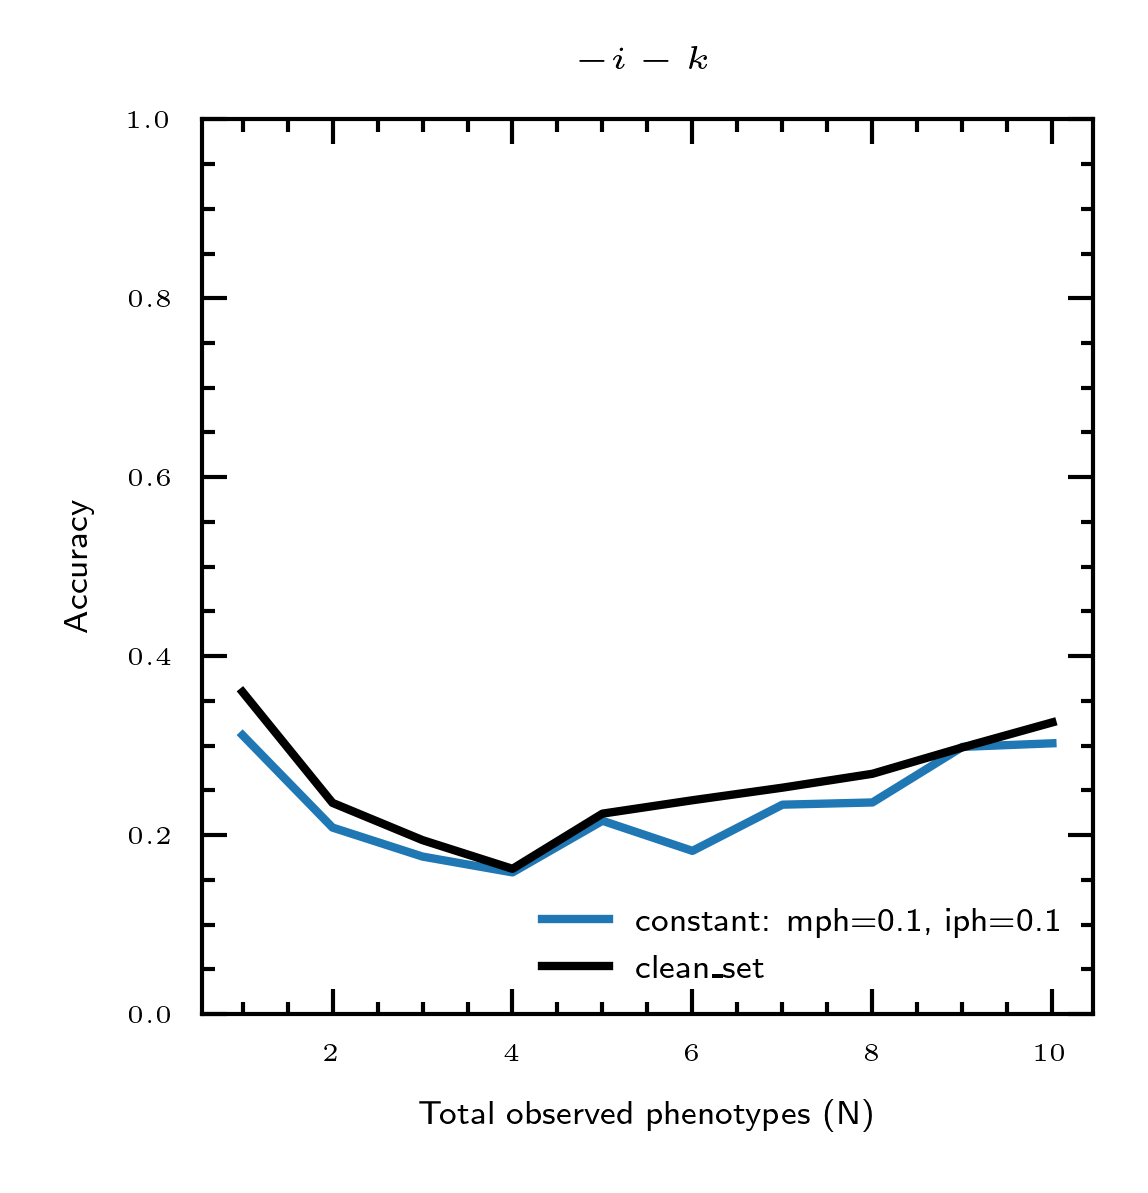
\includegraphics{docs/-i-k.png} \caption{Caption for docs/-i-k.png.} \end{figure}
\begin{figure}[h] \centering 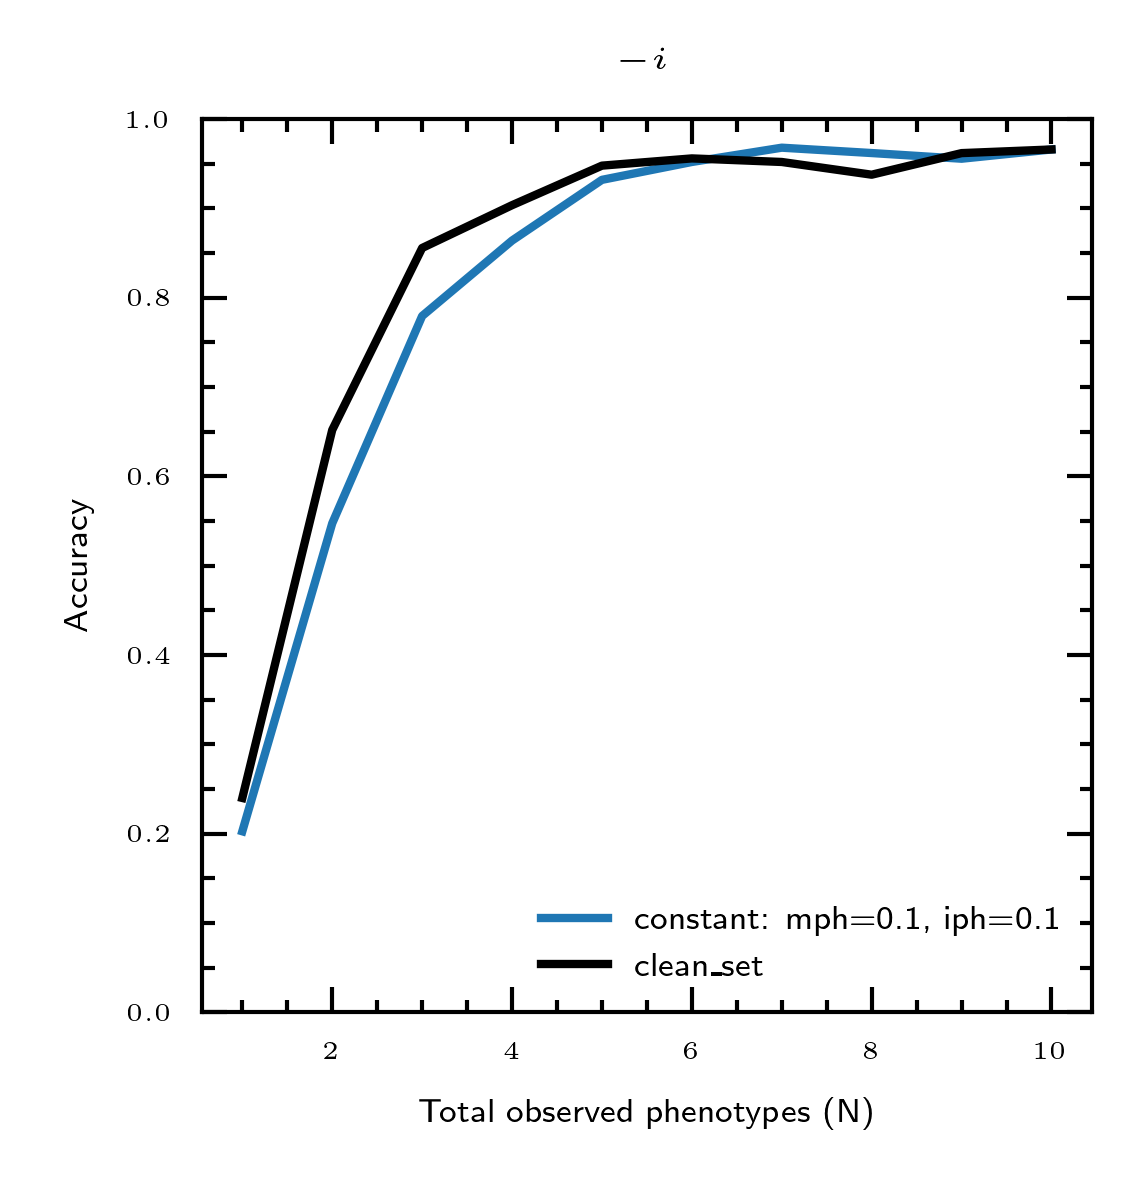
\includegraphics{docs/-i_solo.png} \caption{Caption for docs/-i_solo.png.} \end{figure}
\begin{figure}[h] \centering 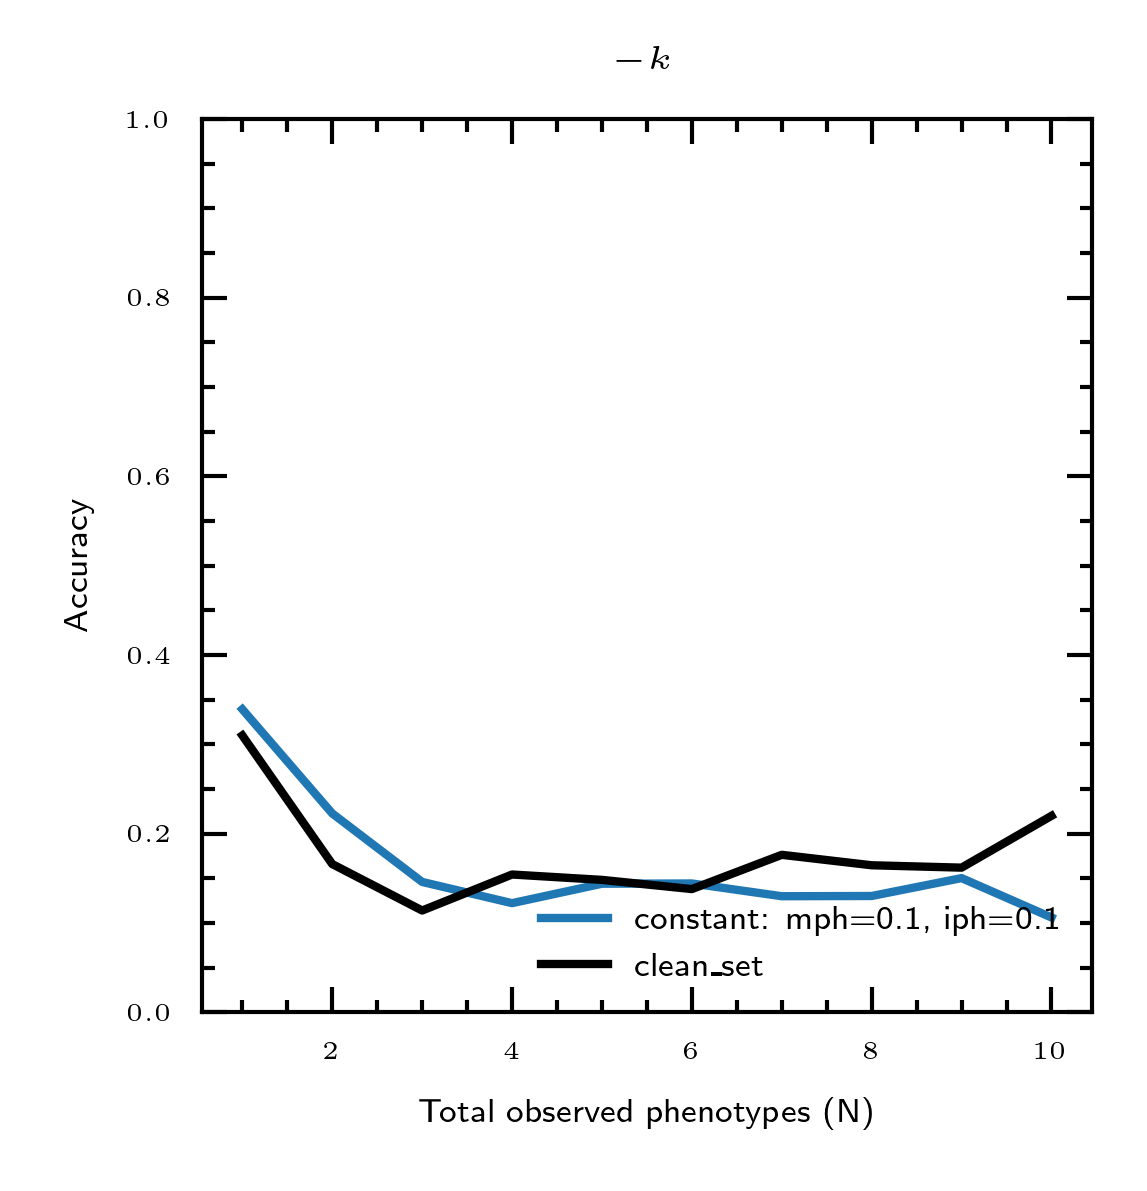
\includegraphics{docs/-k_solo.png} \caption{Caption for docs/-k_solo.png.} \end{figure}
\begin{figure}[h] \centering 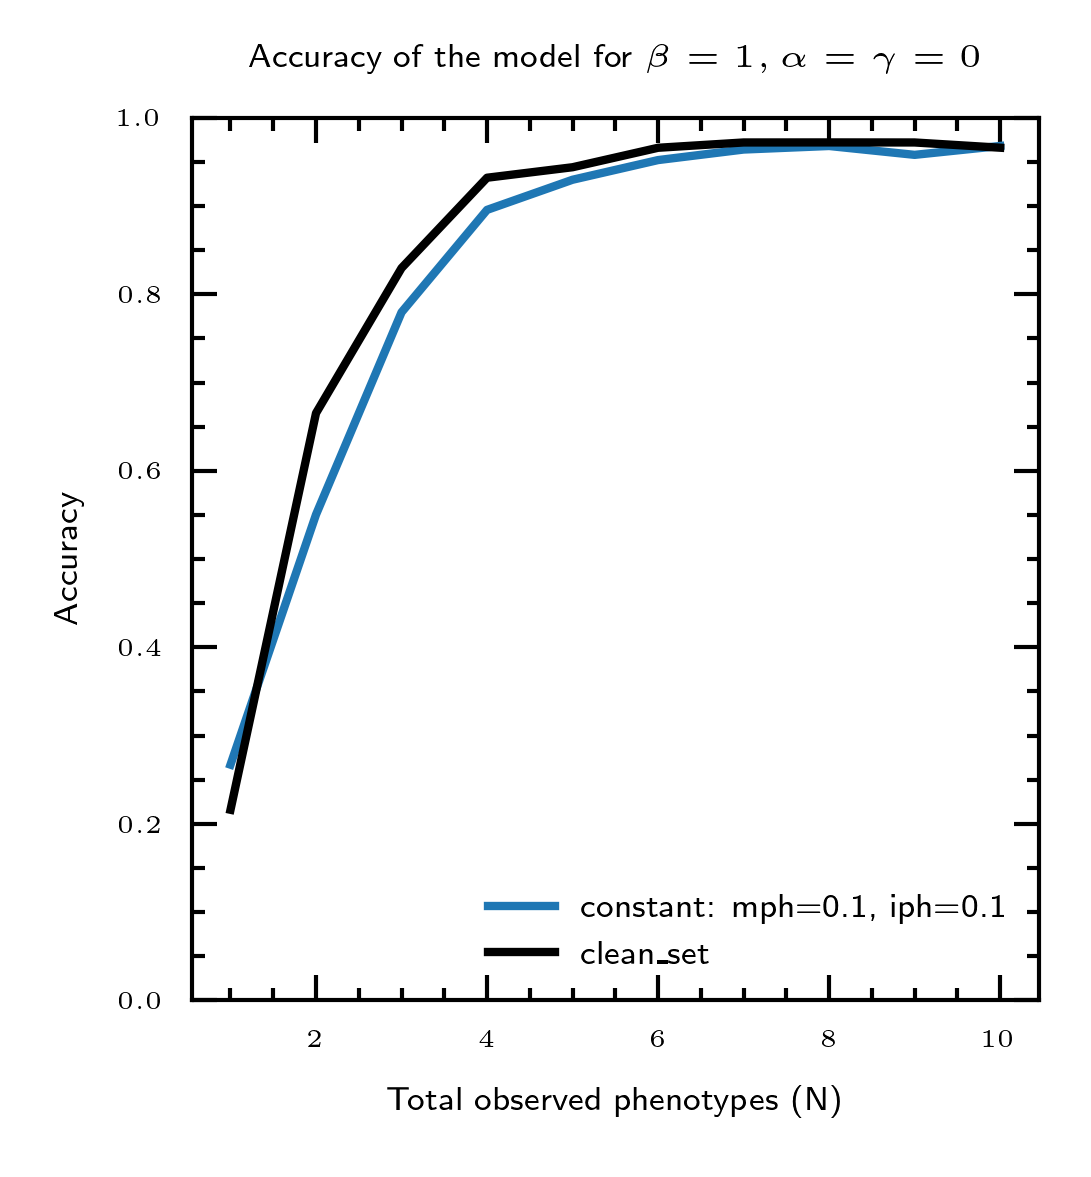
\includegraphics{docs/Accuracy_capitalidad.png} \caption{Caption for docs/Accuracy_capitalidad.png.} \end{figure}
\begin{figure}[h] \centering 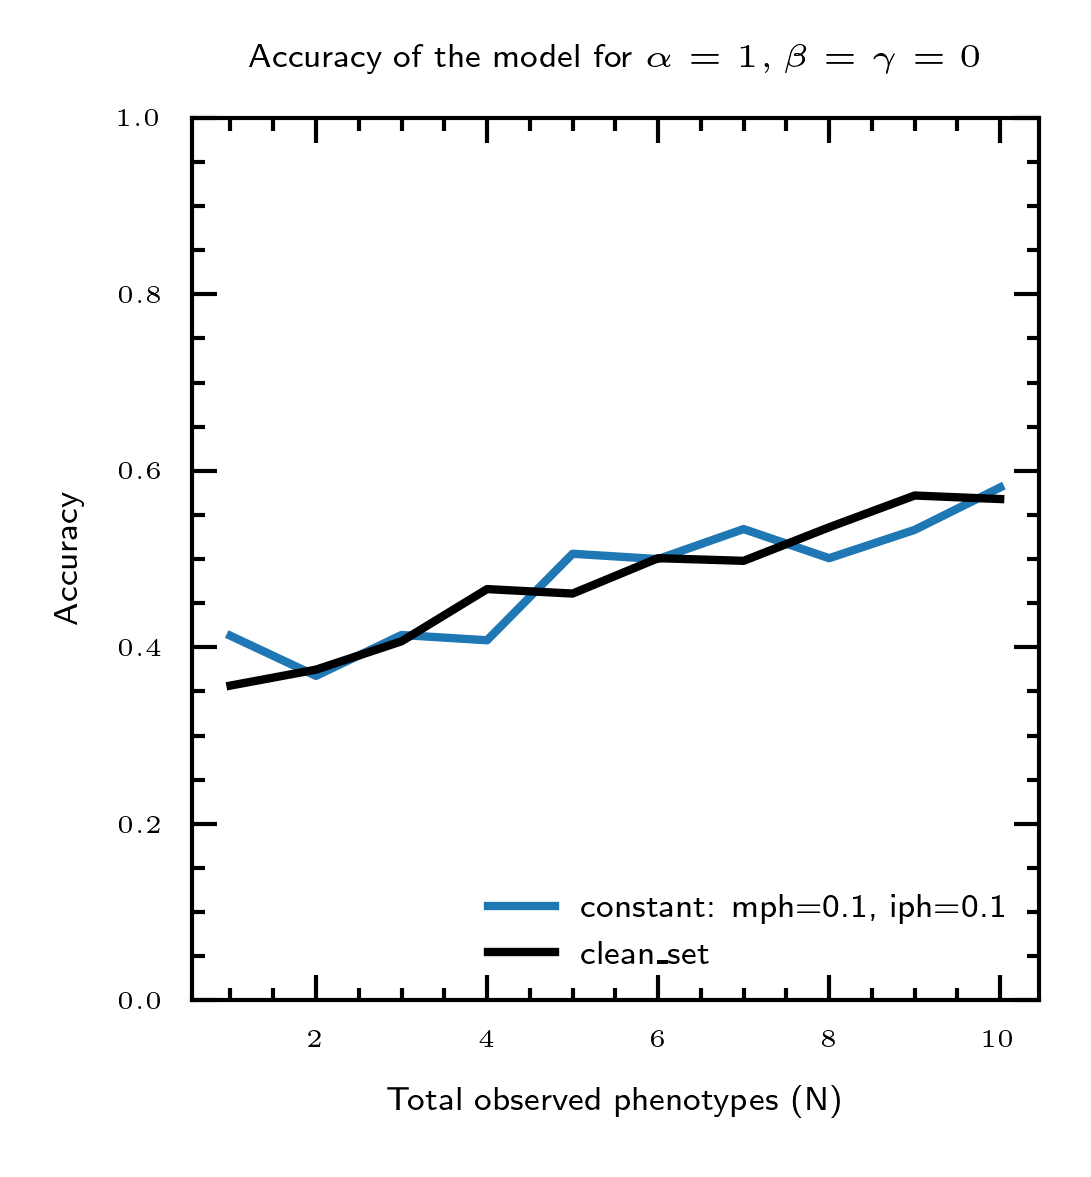
\includegraphics{docs/Accuracy_especificidad.png} \caption{Caption for docs/Accuracy_especificidad.png.} \end{figure}
\begin{figure}[h] \centering 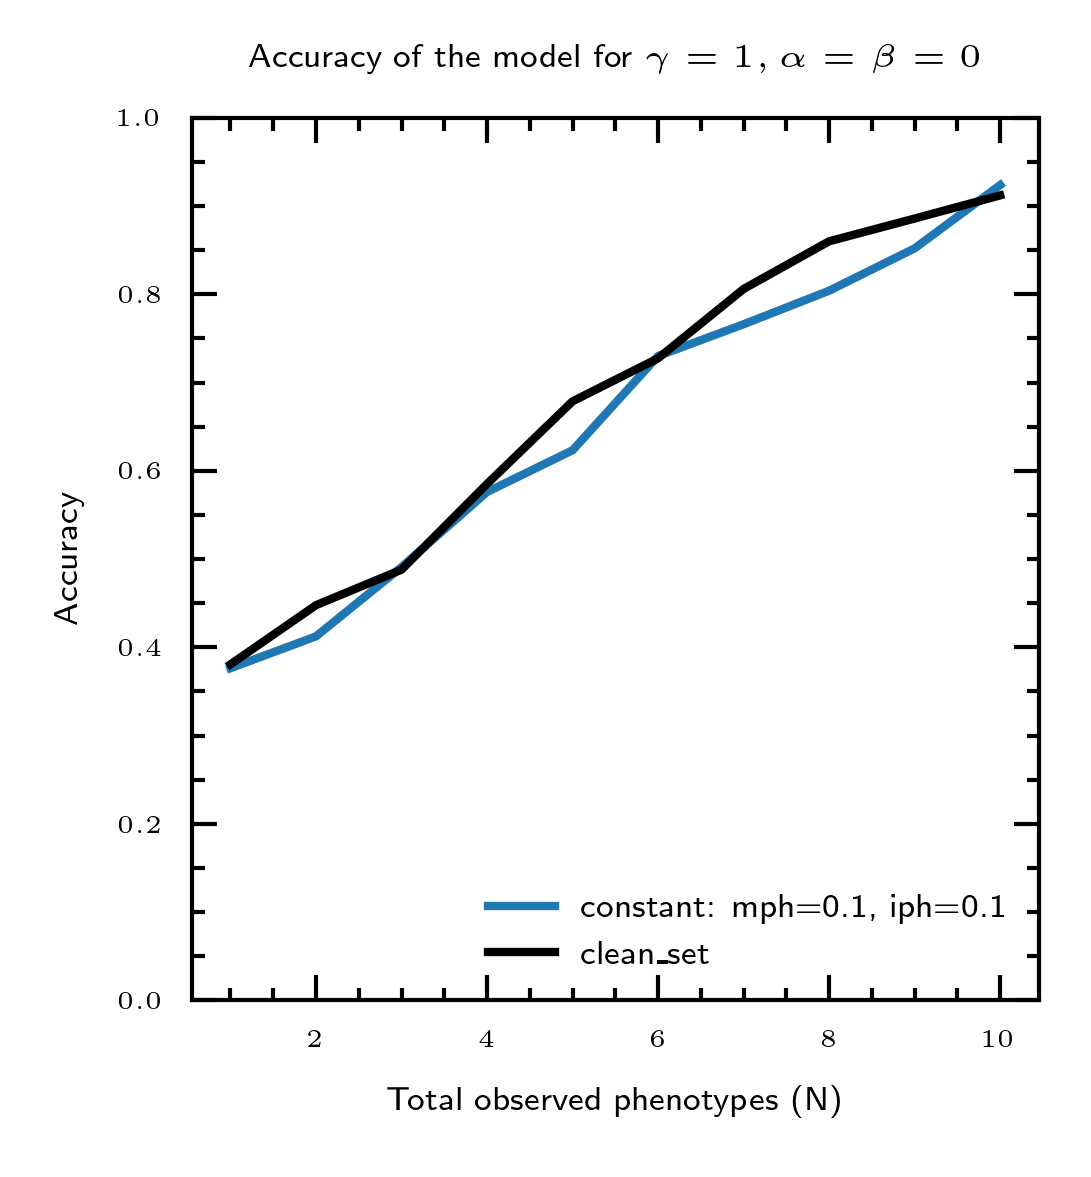
\includegraphics{docs/Accuracy_similaridad.png} \caption{Caption for docs/Accuracy_similaridad.png.} \end{figure}
\begin{figure}[h] \centering \includegraphics{docs/cap_mas_esp_mas_sim.png} \caption{Caption for docs/cap_mas_esp_mas_sim.png.} \end{figure}
\begin{figure}[h] \centering \includegraphics{docs/cap_mas_sim.png} \caption{Caption for docs/cap_mas_sim.png.} \end{figure}
\begin{figure}[h] \centering 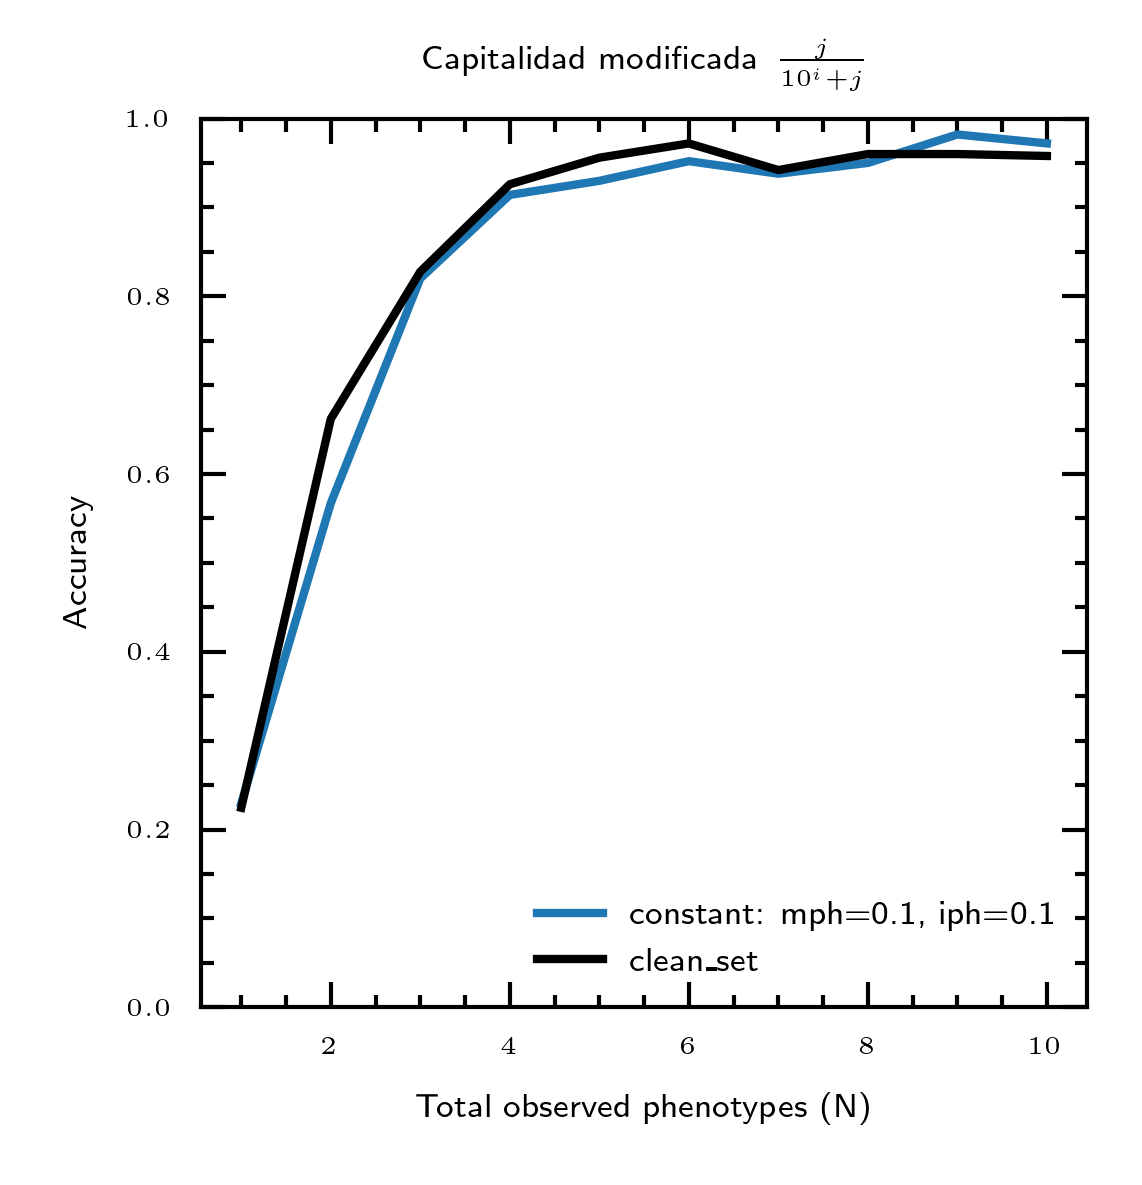
\includegraphics{docs/capitalidad_accuracy_exponencial.png} \caption{Caption for docs/capitalidad_accuracy_exponencial.png.} \end{figure}
\begin{figure}[h] \centering 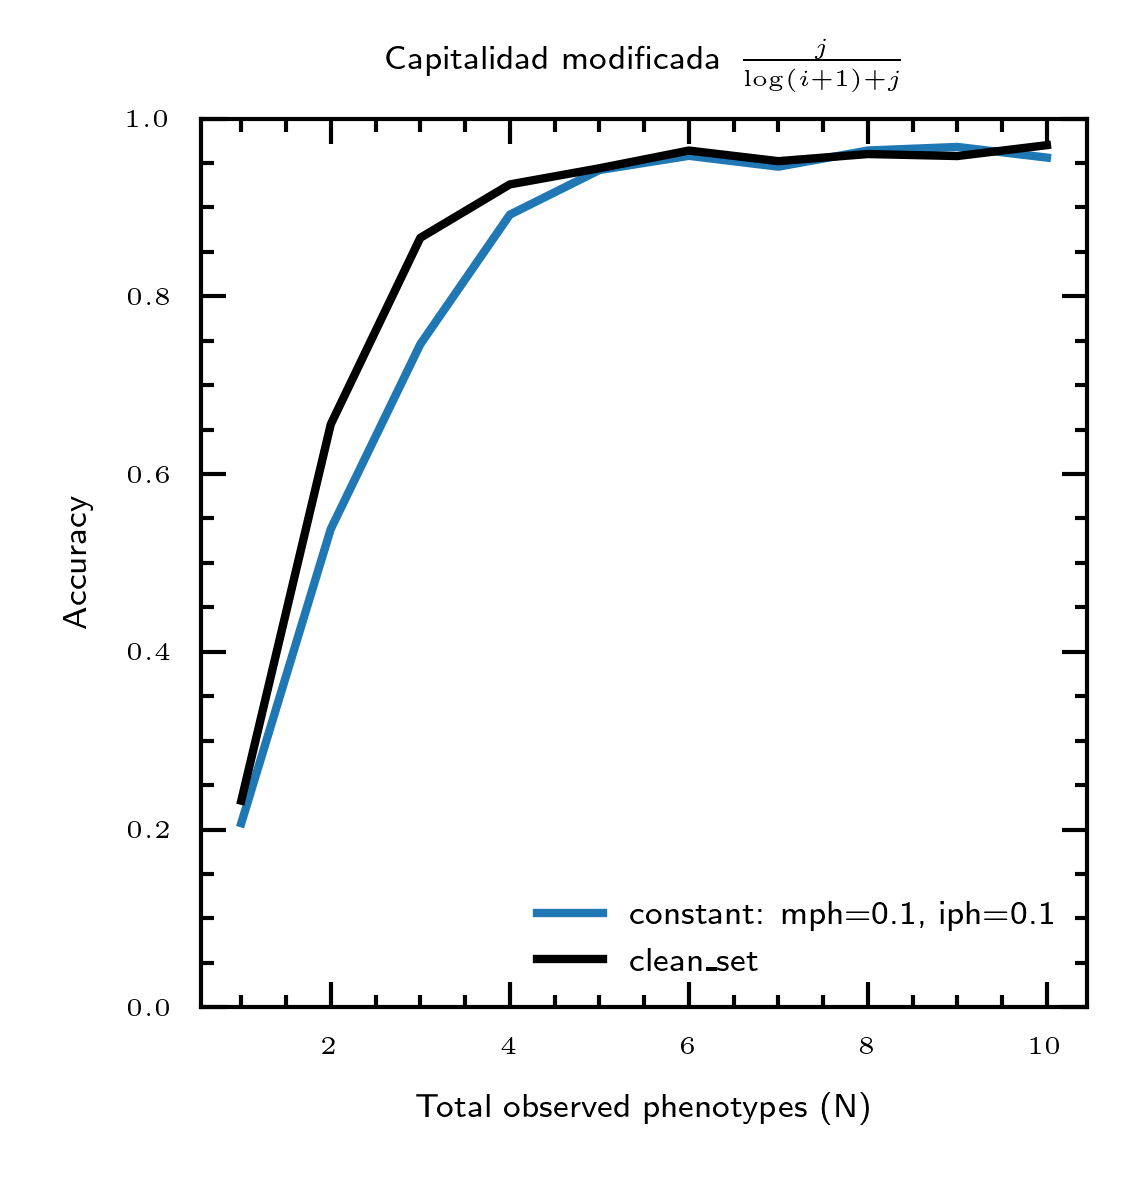
\includegraphics{docs/capitalidad_accuracy_logaritmico.png} \caption{Caption for docs/capitalidad_accuracy_logaritmico.png.} \end{figure}
\begin{figure}[h] \centering \includegraphics{docs/esp_mas_cap.png} \caption{Caption for docs/esp_mas_cap.png.} \end{figure}
\begin{figure}[h] \centering \includegraphics{docs/esp_mas_sim.png} \caption{Caption for docs/esp_mas_sim.png.} \end{figure}
\begin{figure}[h] \centering 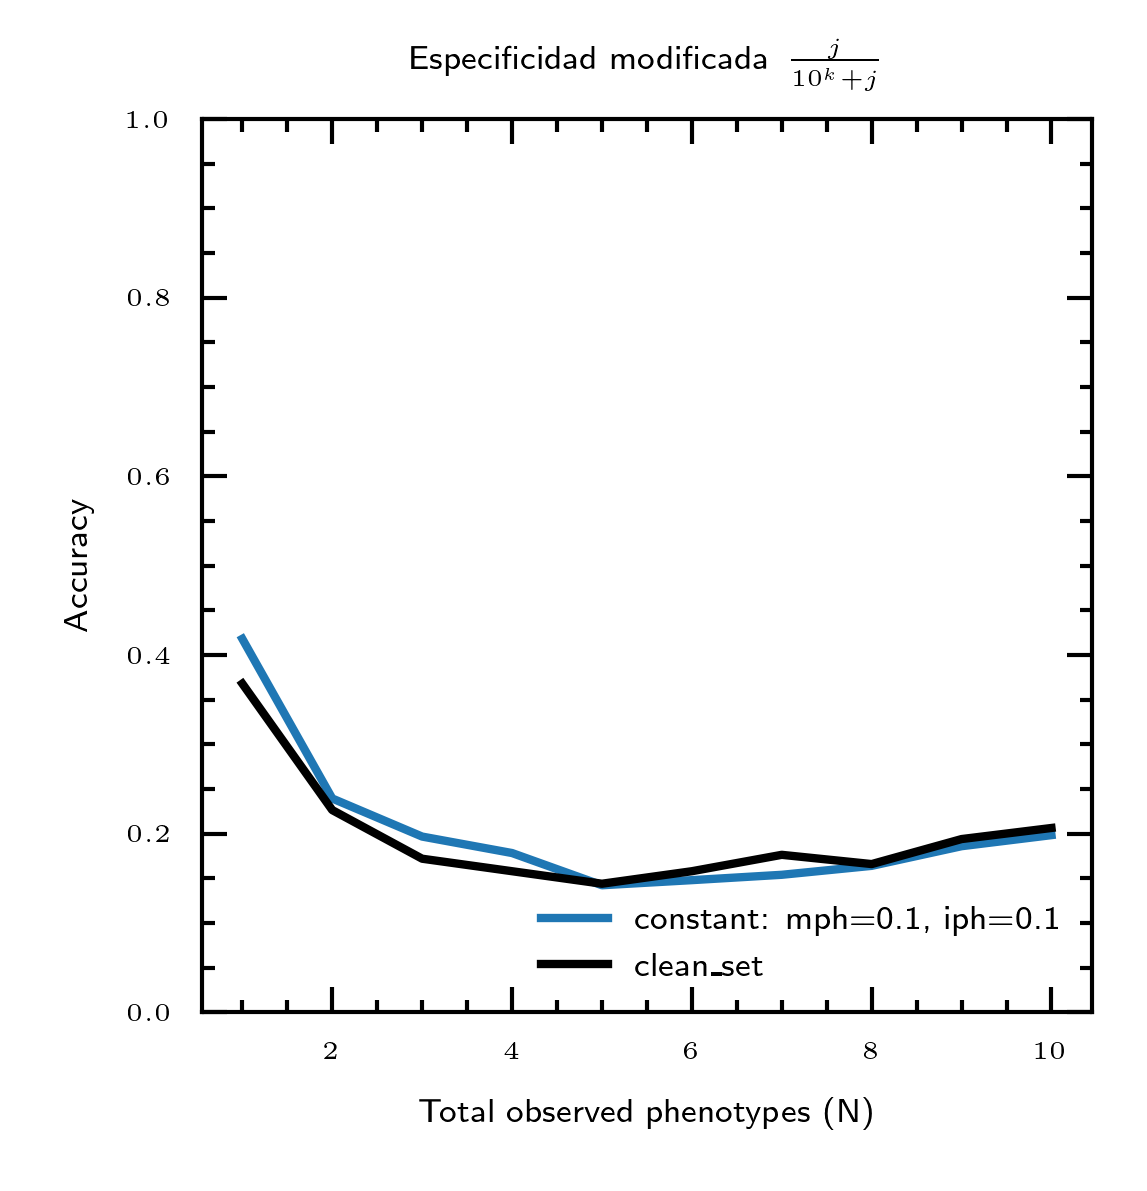
\includegraphics{docs/especificidad_accuracy_exponencial.png} \caption{Caption for docs/especificidad_accuracy_exponencial.png.} \end{figure}
\begin{figure}[h] \centering 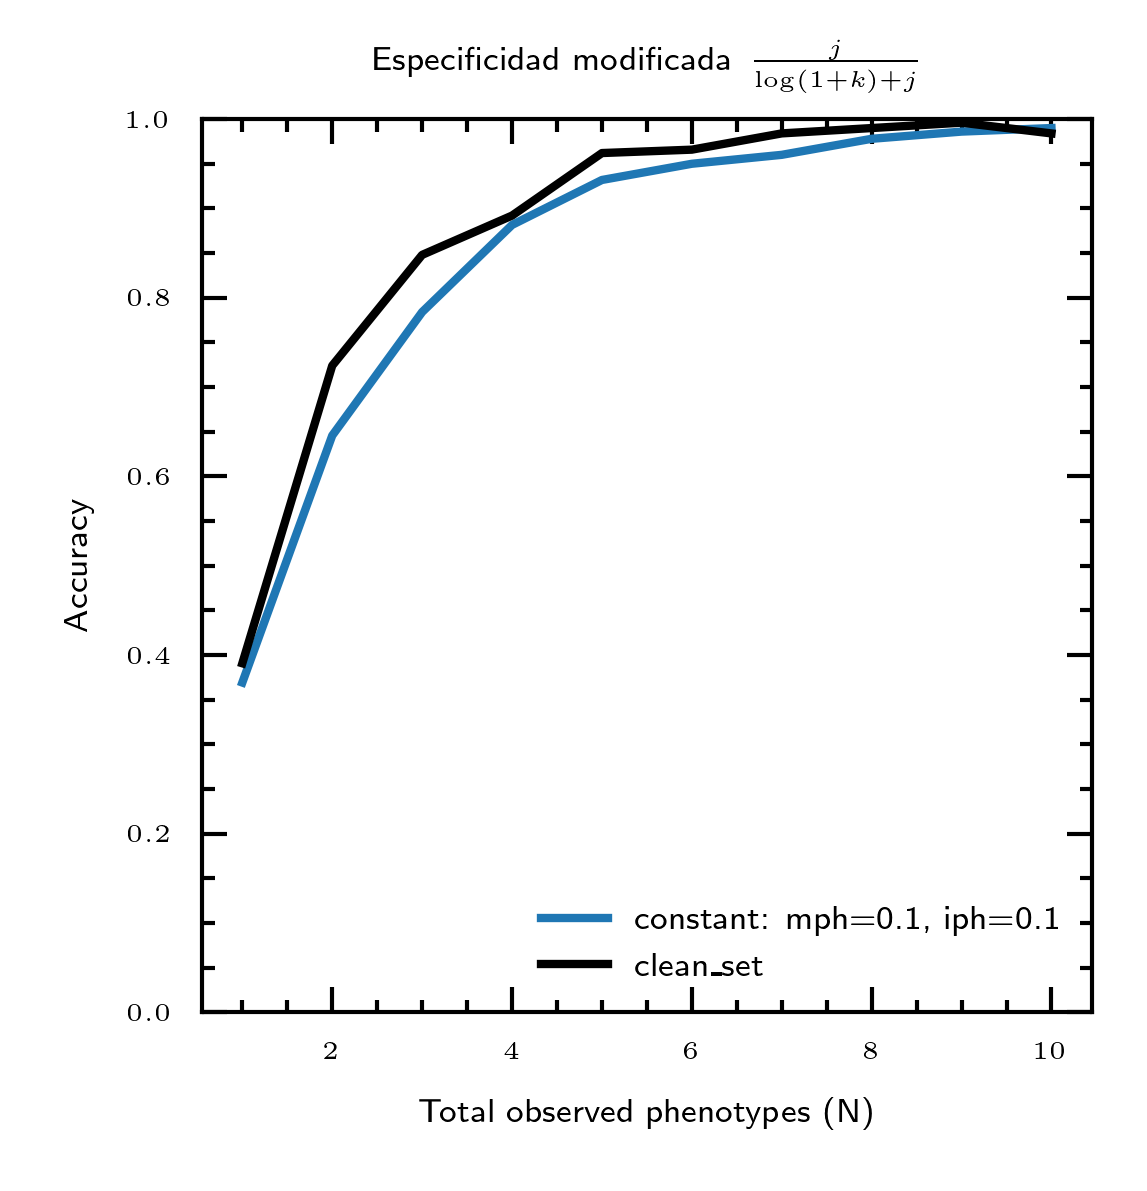
\includegraphics{docs/especificidad_accuracy_logaritmico.png} \caption{Caption for docs/especificidad_accuracy_logaritmico.png.} \end{figure}
\begin{figure}[h] \centering 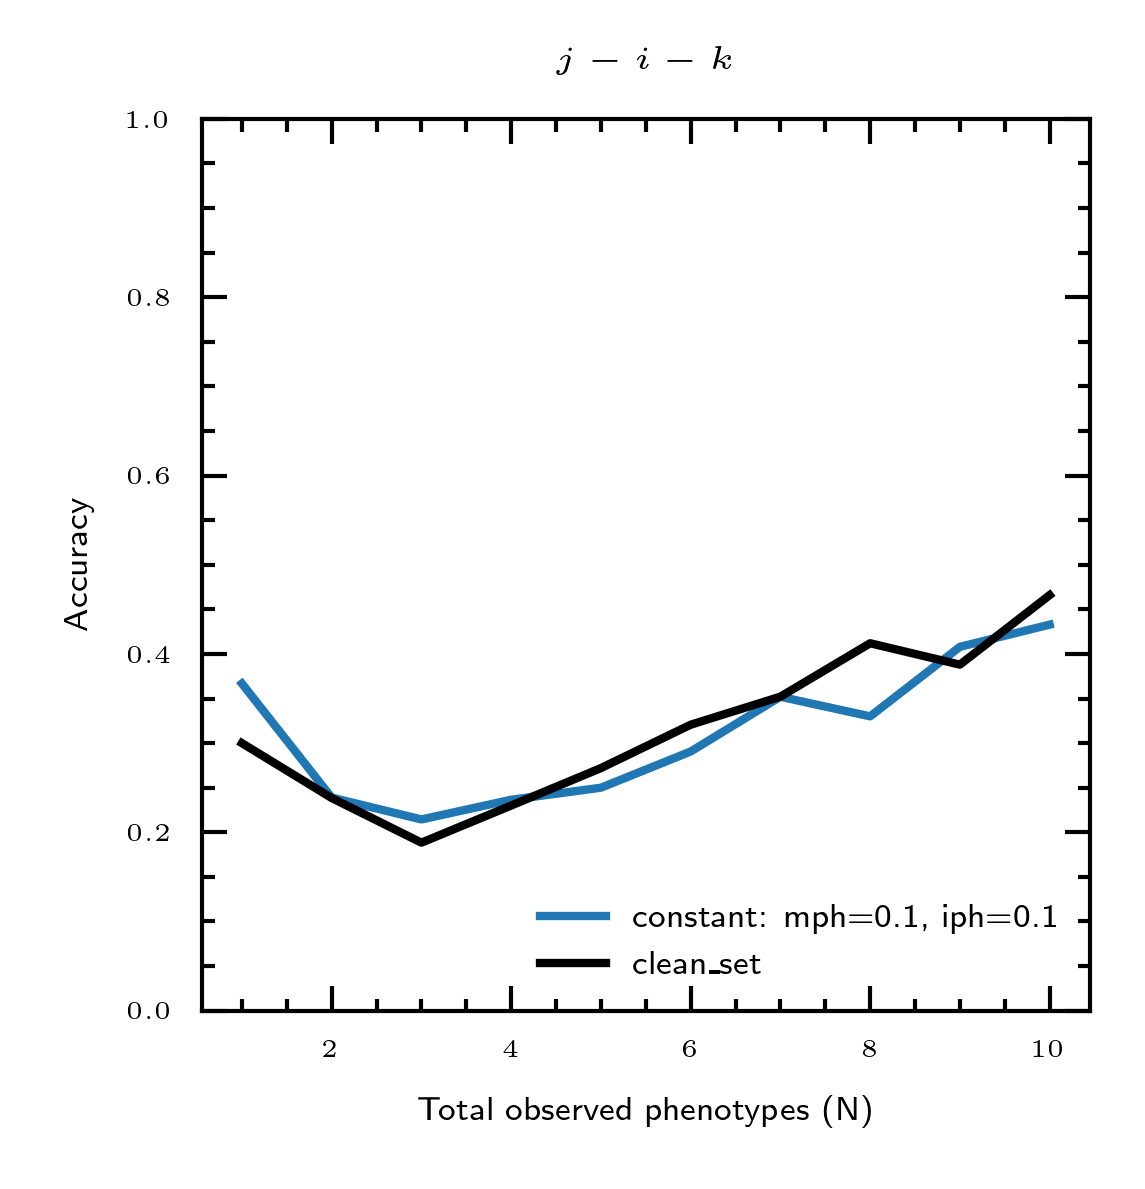
\includegraphics{docs/j-i-k.png} \caption{Caption for docs/j-i-k.png.} \end{figure}
\begin{figure}[h] \centering 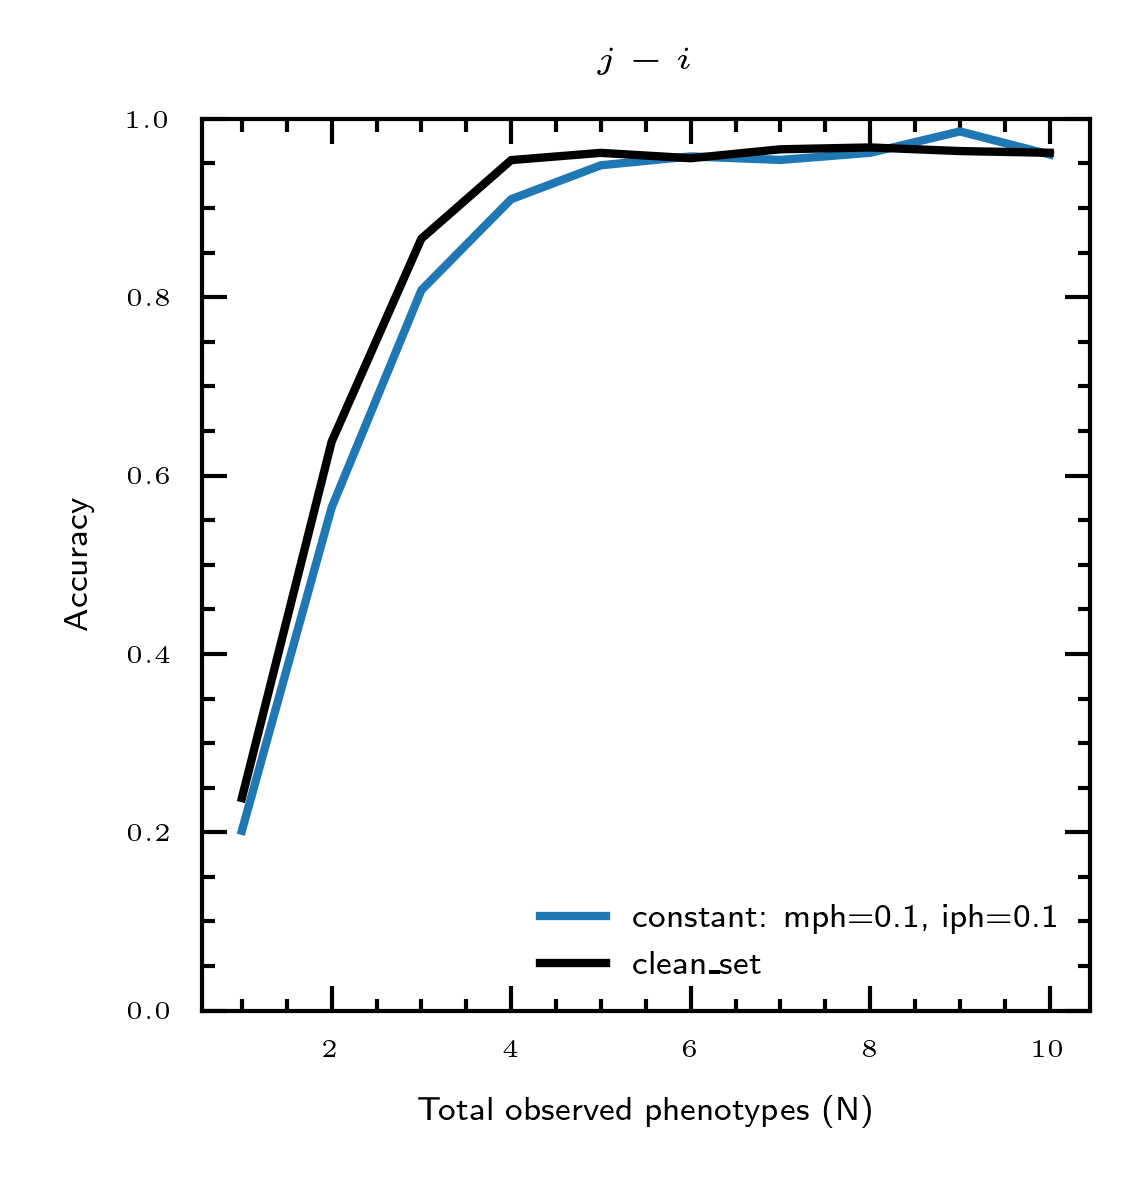
\includegraphics{docs/j-i.png} \caption{Caption for docs/j-i.png.} \end{figure}
\begin{figure}[h] \centering 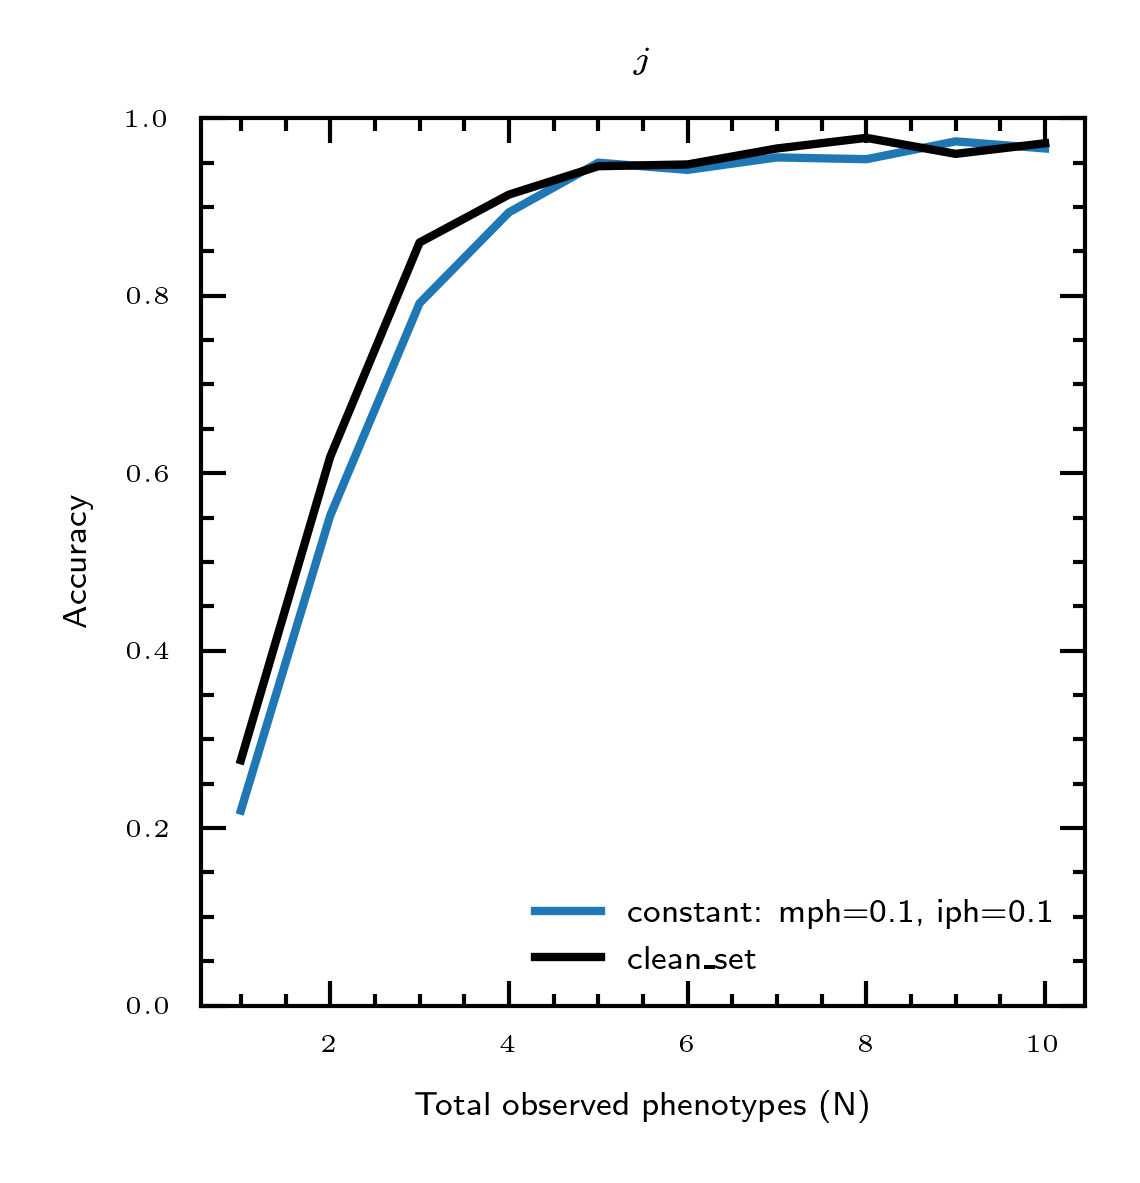
\includegraphics{docs/j_solo.png} \caption{Caption for docs/j_solo.png.} \end{figure}
\begin{figure}[h] \centering 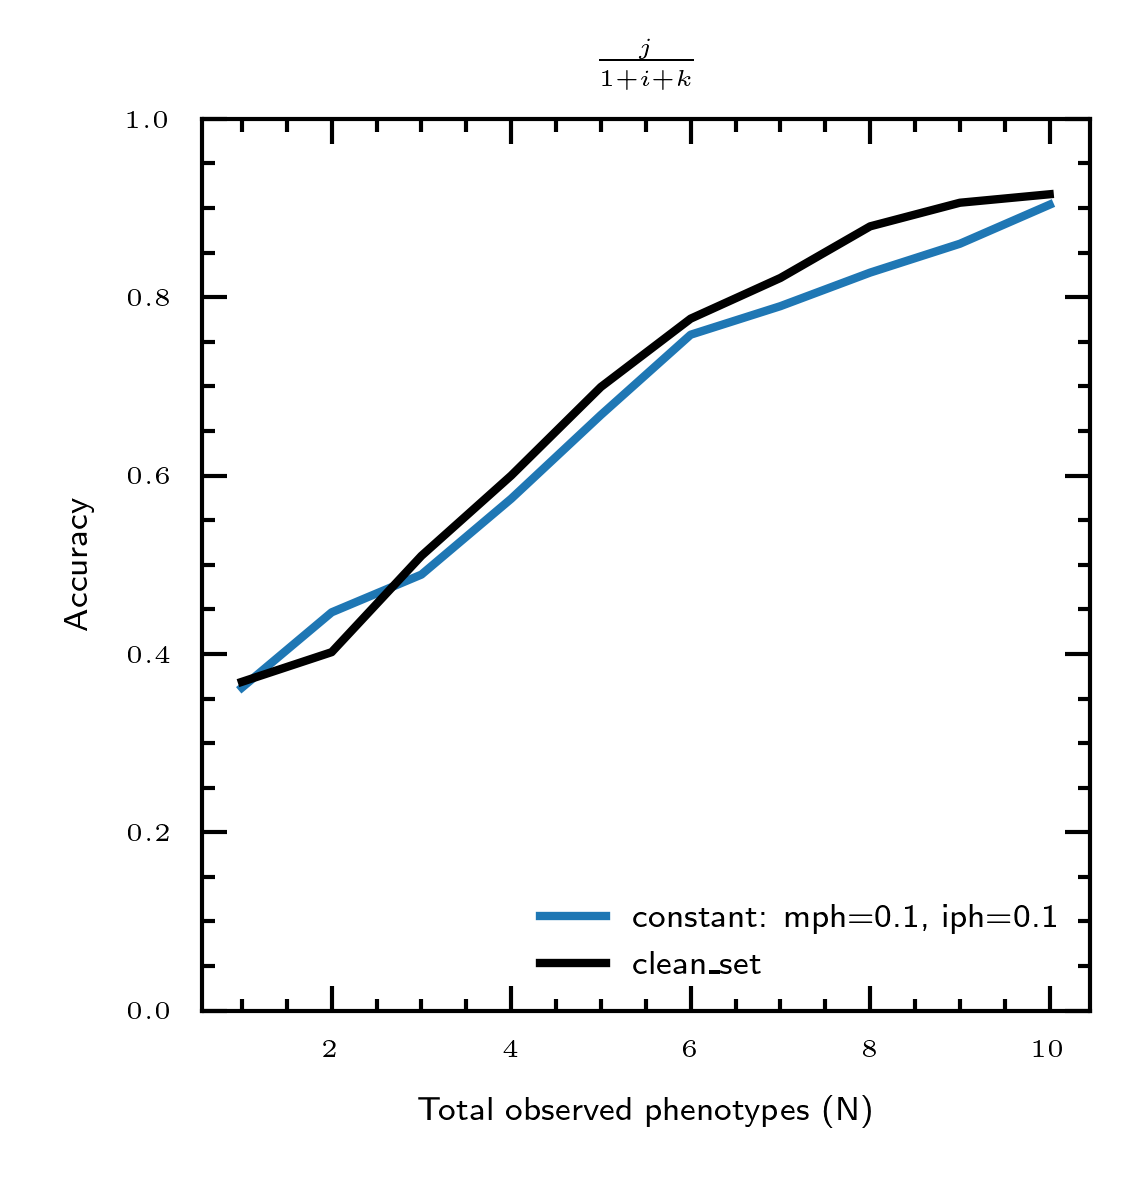
\includegraphics{docs/jsobre1+i+k.png} \caption{Caption for docs/jsobre1+i+k.png.} \end{figure}
\begin{figure}[h] \centering 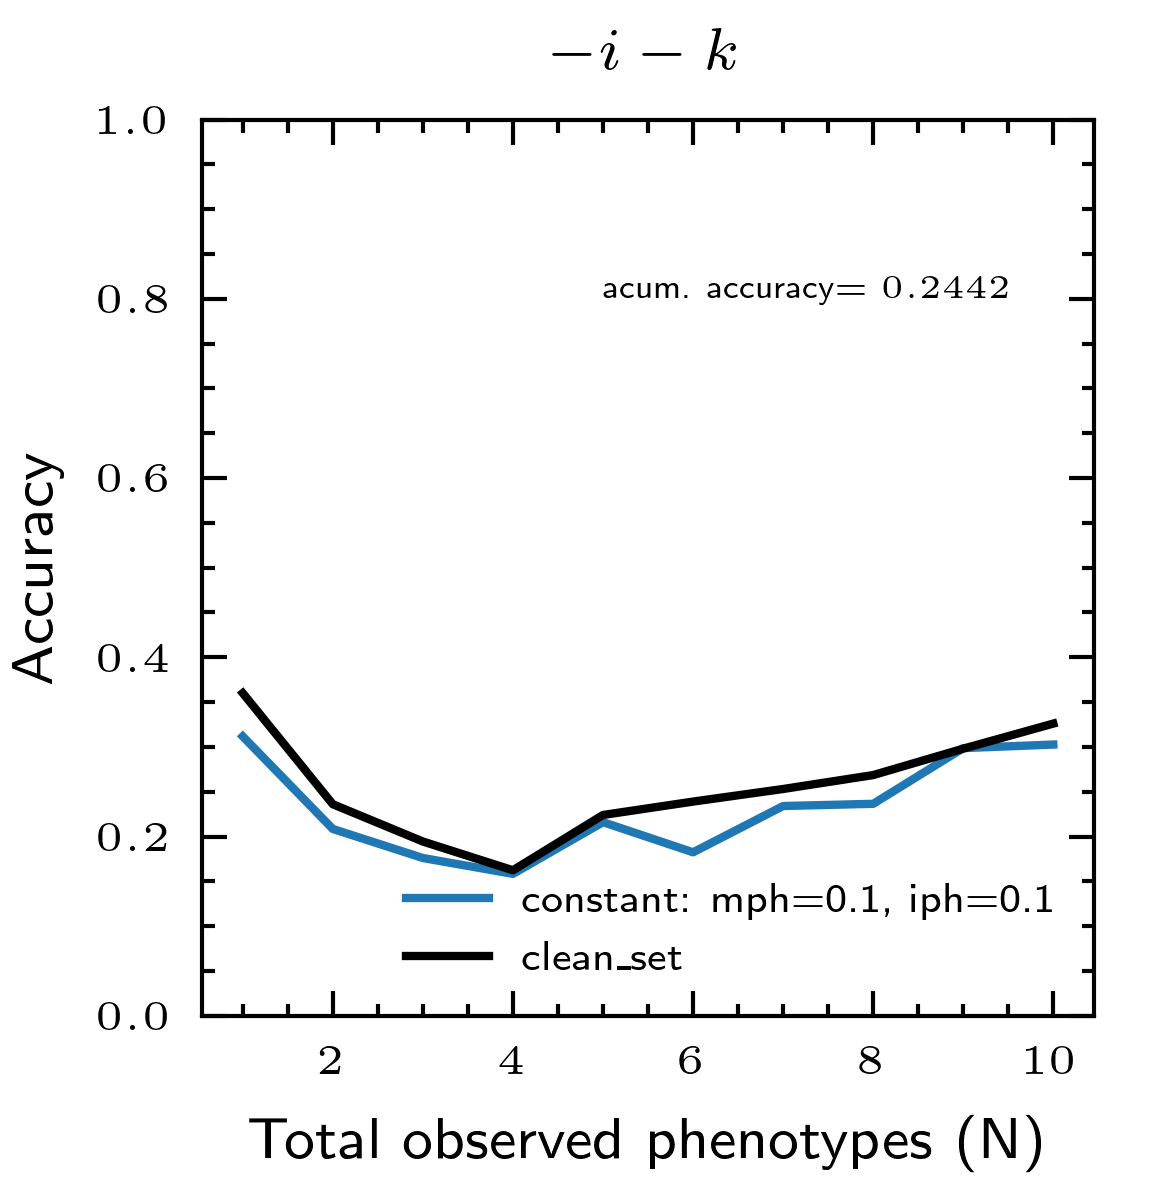
\includegraphics{docs/metrics_evaluation/-i-k.png} \caption{Caption for docs/metrics_evaluation/-i-k.png.} \end{figure}
\begin{figure}[h] \centering 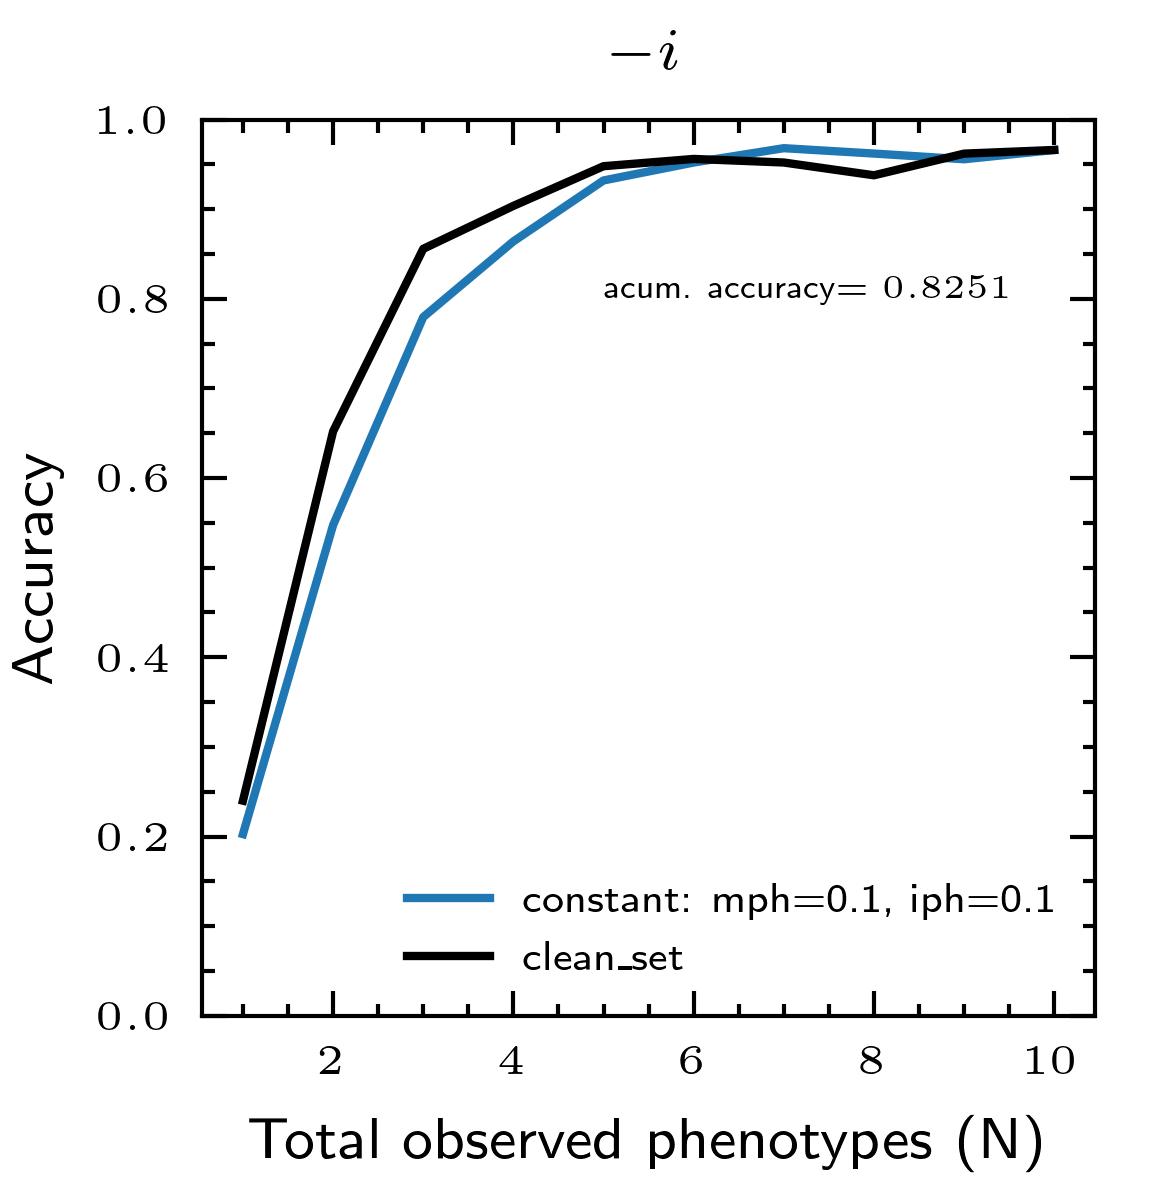
\includegraphics{docs/metrics_evaluation/-i_solo.png} \caption{Caption for docs/metrics_evaluation/-i_solo.png.} \end{figure}
\begin{figure}[h] \centering 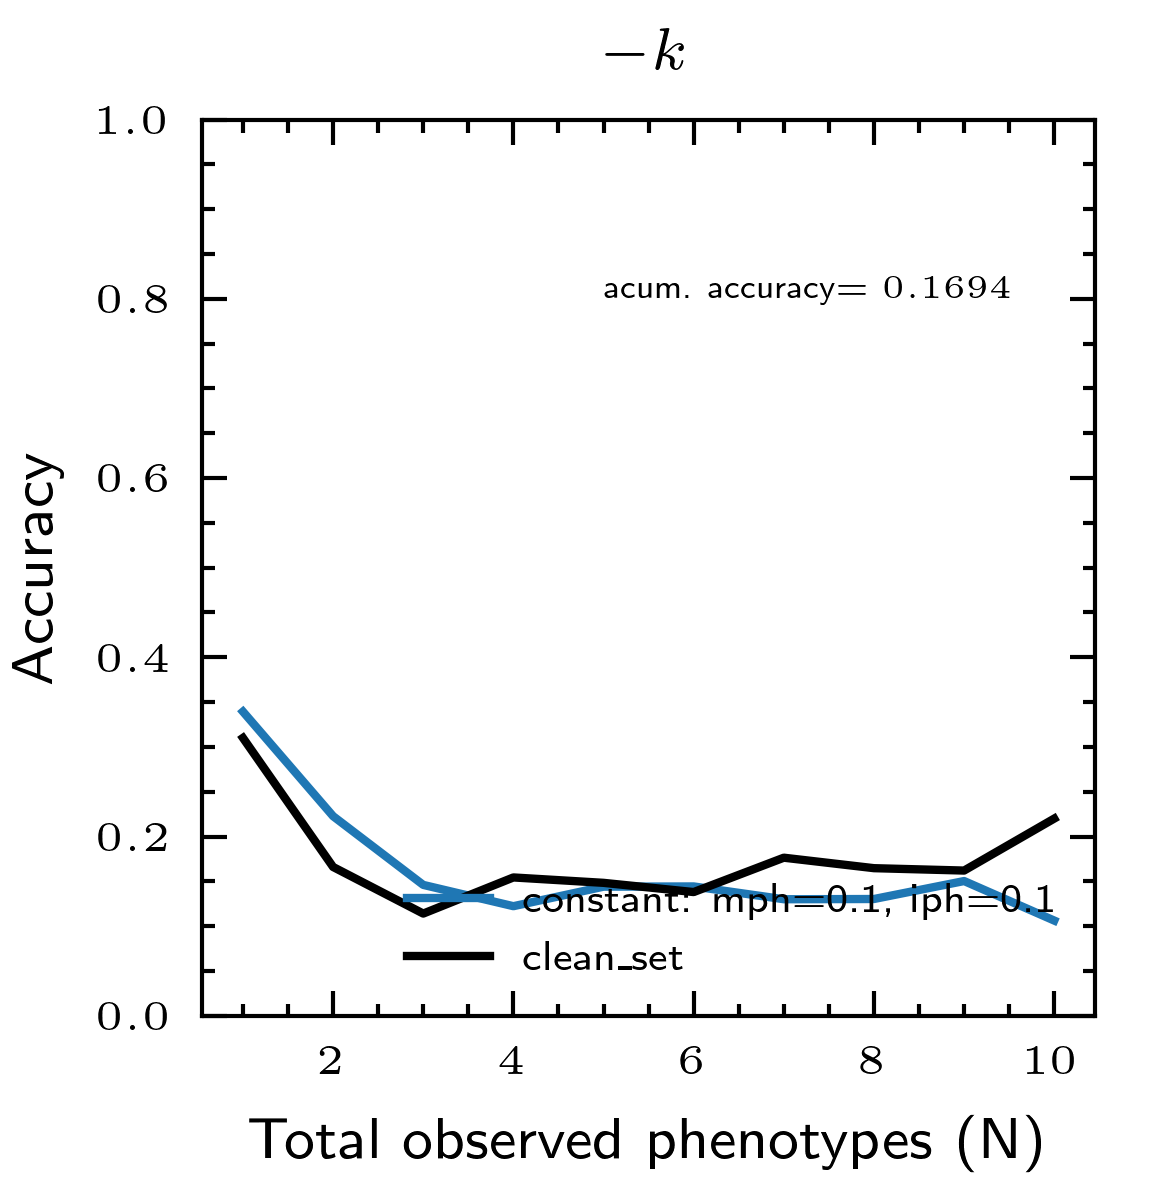
\includegraphics{docs/metrics_evaluation/-k_solo.png} \caption{Caption for docs/metrics_evaluation/-k_solo.png.} \end{figure}
\begin{figure}[h] \centering \includegraphics{docs/metrics_evaluation/cap_mas_esp_mas_sim.png} \caption{Caption for docs/metrics_evaluation/cap_mas_esp_mas_sim.png.} \end{figure}
\begin{figure}[h] \centering \includegraphics{docs/metrics_evaluation/cap_mas_sim.png} \caption{Caption for docs/metrics_evaluation/cap_mas_sim.png.} \end{figure}
\begin{figure}[h] \centering 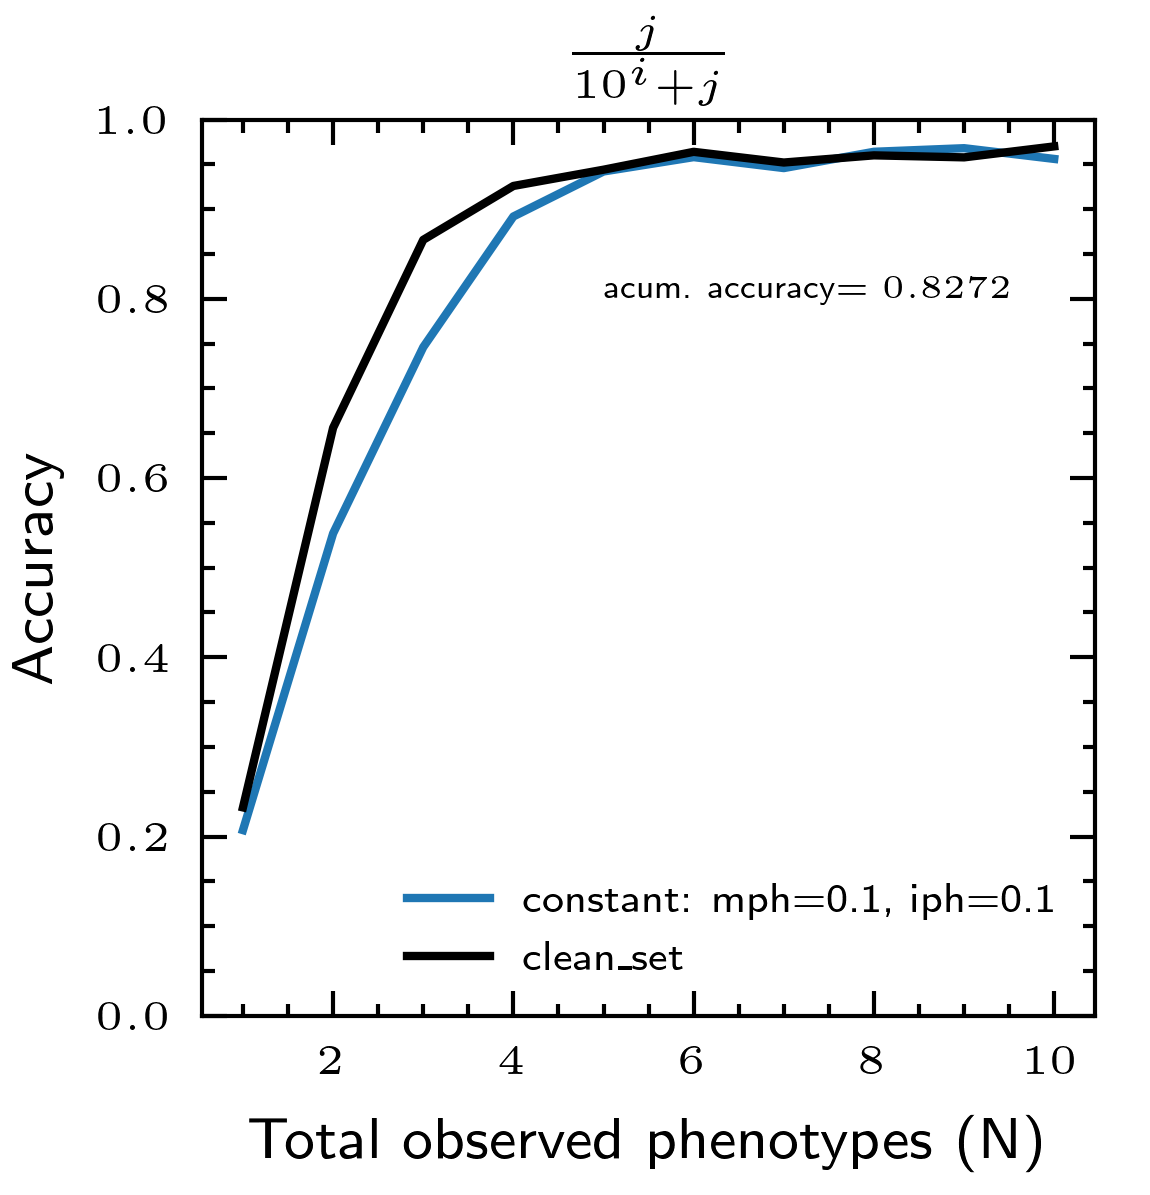
\includegraphics{docs/metrics_evaluation/capitalidad_accuracy_exponencial.png} \caption{Caption for docs/metrics_evaluation/capitalidad_accuracy_exponencial.png.} \end{figure}
\begin{figure}[h] \centering 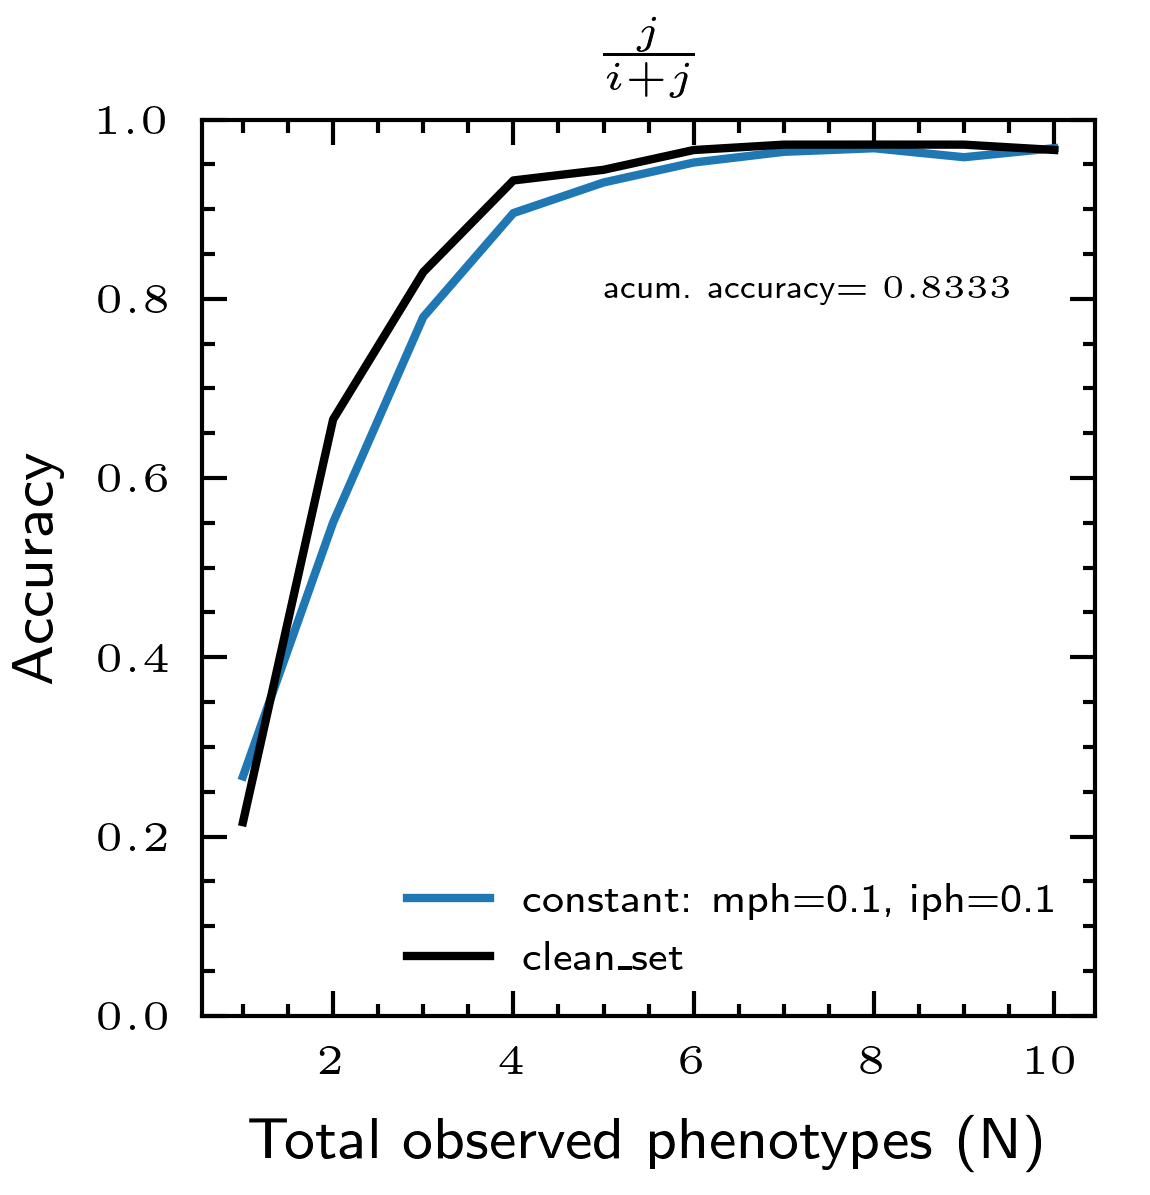
\includegraphics{docs/metrics_evaluation/capitalidad_accuracy_lineal.png} \caption{Caption for docs/metrics_evaluation/capitalidad_accuracy_lineal.png.} \end{figure}
\begin{figure}[h] \centering 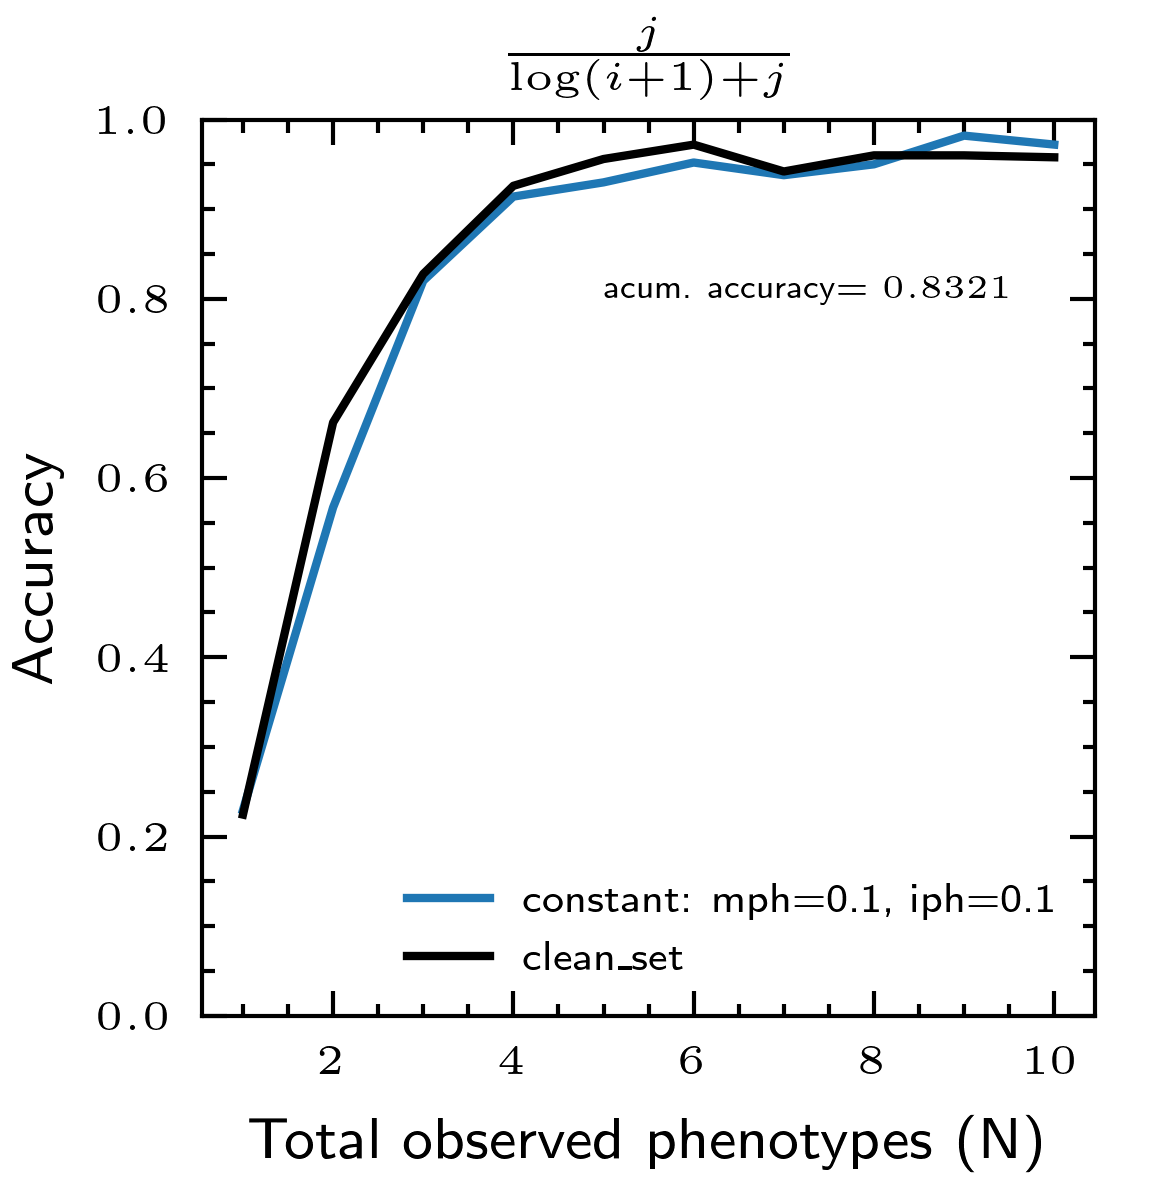
\includegraphics{docs/metrics_evaluation/capitalidad_accuracy_logaritmico.png} \caption{Caption for docs/metrics_evaluation/capitalidad_accuracy_logaritmico.png.} \end{figure}
\begin{figure}[h] \centering \includegraphics{docs/metrics_evaluation/esp_mas_cap.png} \caption{Caption for docs/metrics_evaluation/esp_mas_cap.png.} \end{figure}
\begin{figure}[h] \centering \includegraphics{docs/metrics_evaluation/esp_mas_sim.png} \caption{Caption for docs/metrics_evaluation/esp_mas_sim.png.} \end{figure}
\begin{figure}[h] \centering 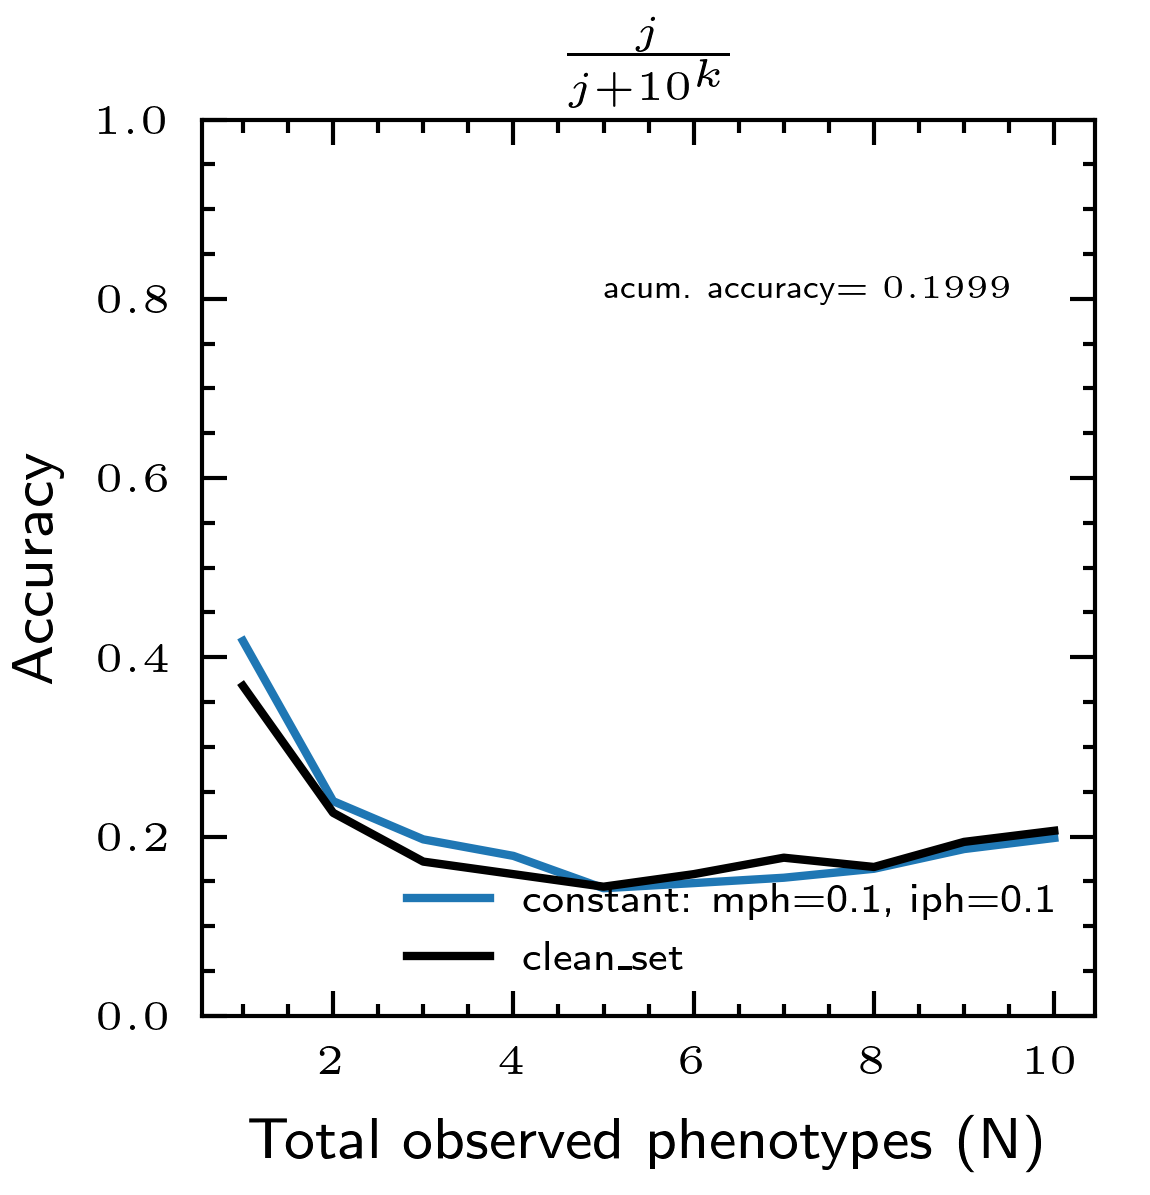
\includegraphics{docs/metrics_evaluation/especificidad_accuracy_exponencial.png} \caption{Caption for docs/metrics_evaluation/especificidad_accuracy_exponencial.png.} \end{figure}
\begin{figure}[h] \centering 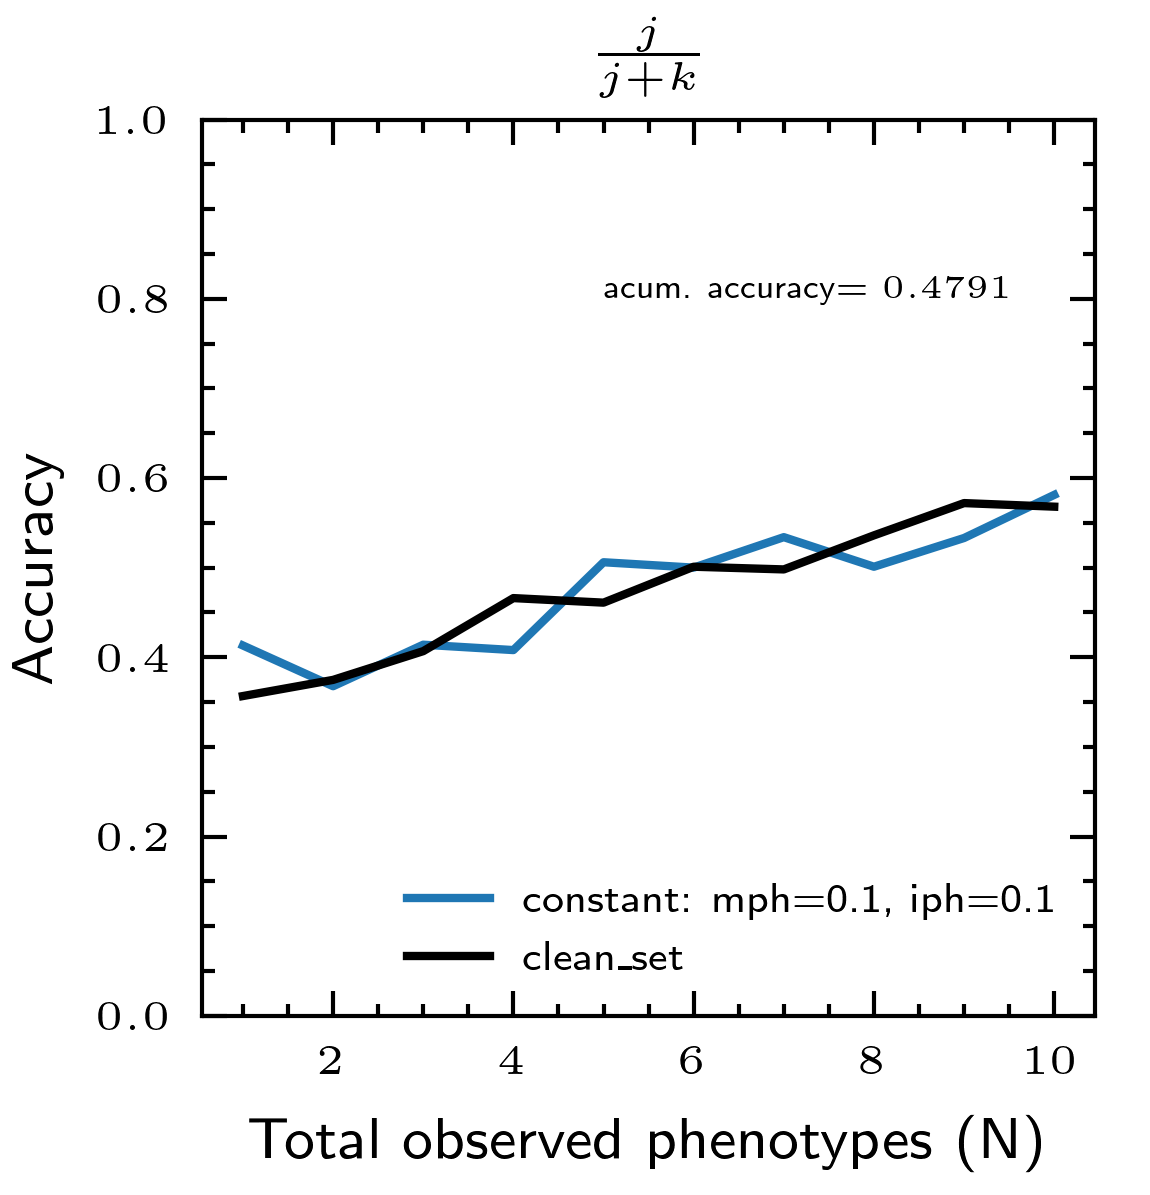
\includegraphics{docs/metrics_evaluation/especificidad_accuracy_lineal.png} \caption{Caption for docs/metrics_evaluation/especificidad_accuracy_lineal.png.} \end{figure}
\begin{figure}[h] \centering 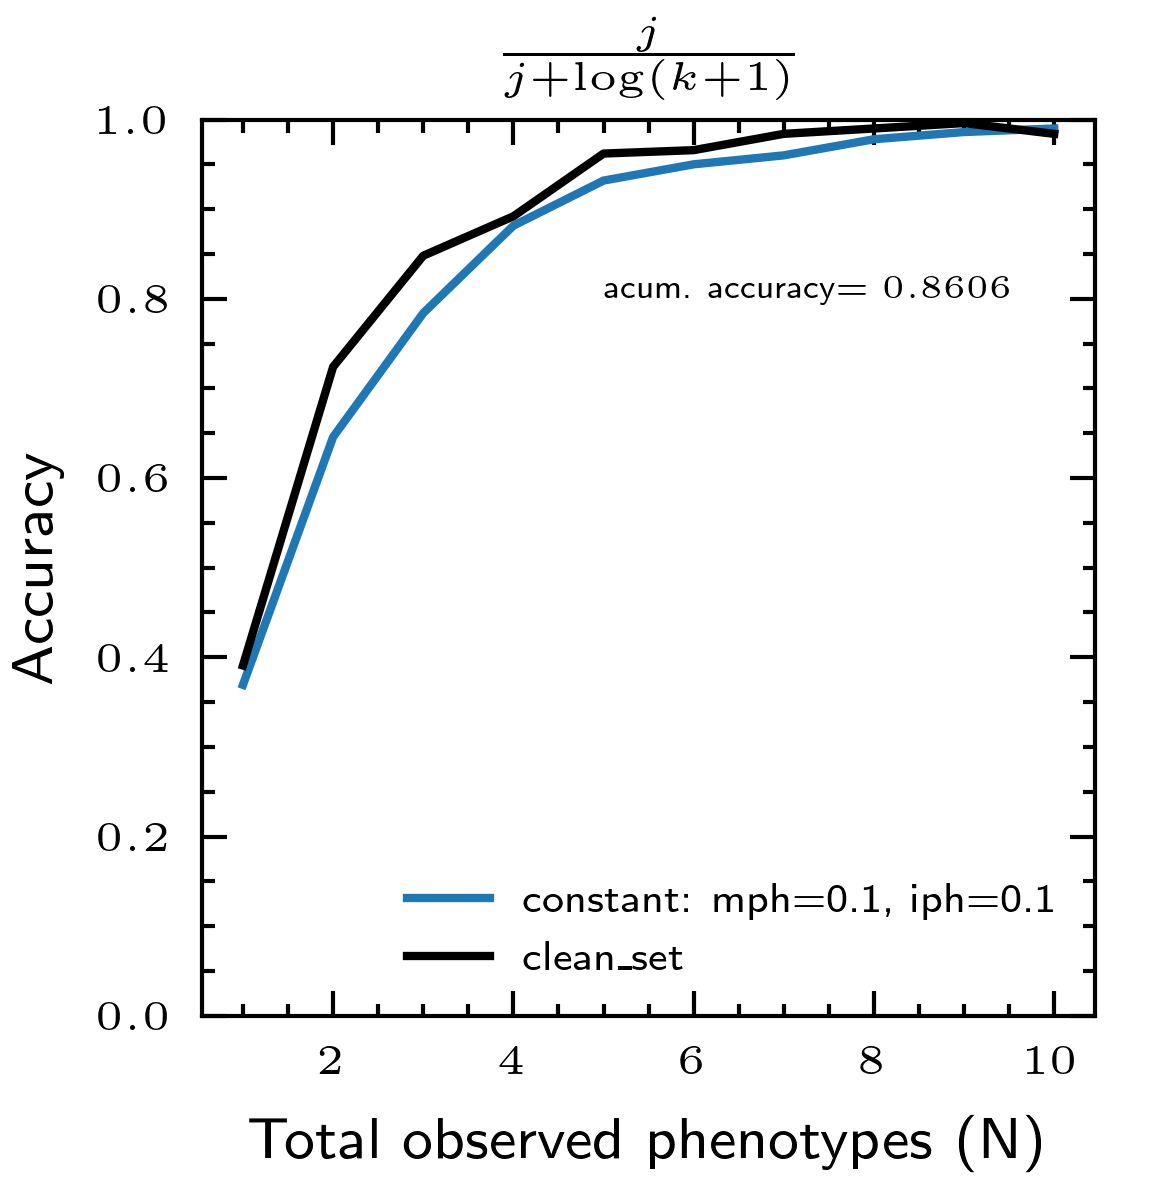
\includegraphics{docs/metrics_evaluation/especificidad_accuracy_logaritmico.png} \caption{Caption for docs/metrics_evaluation/especificidad_accuracy_logaritmico.png.} \end{figure}
\begin{figure}[h] \centering 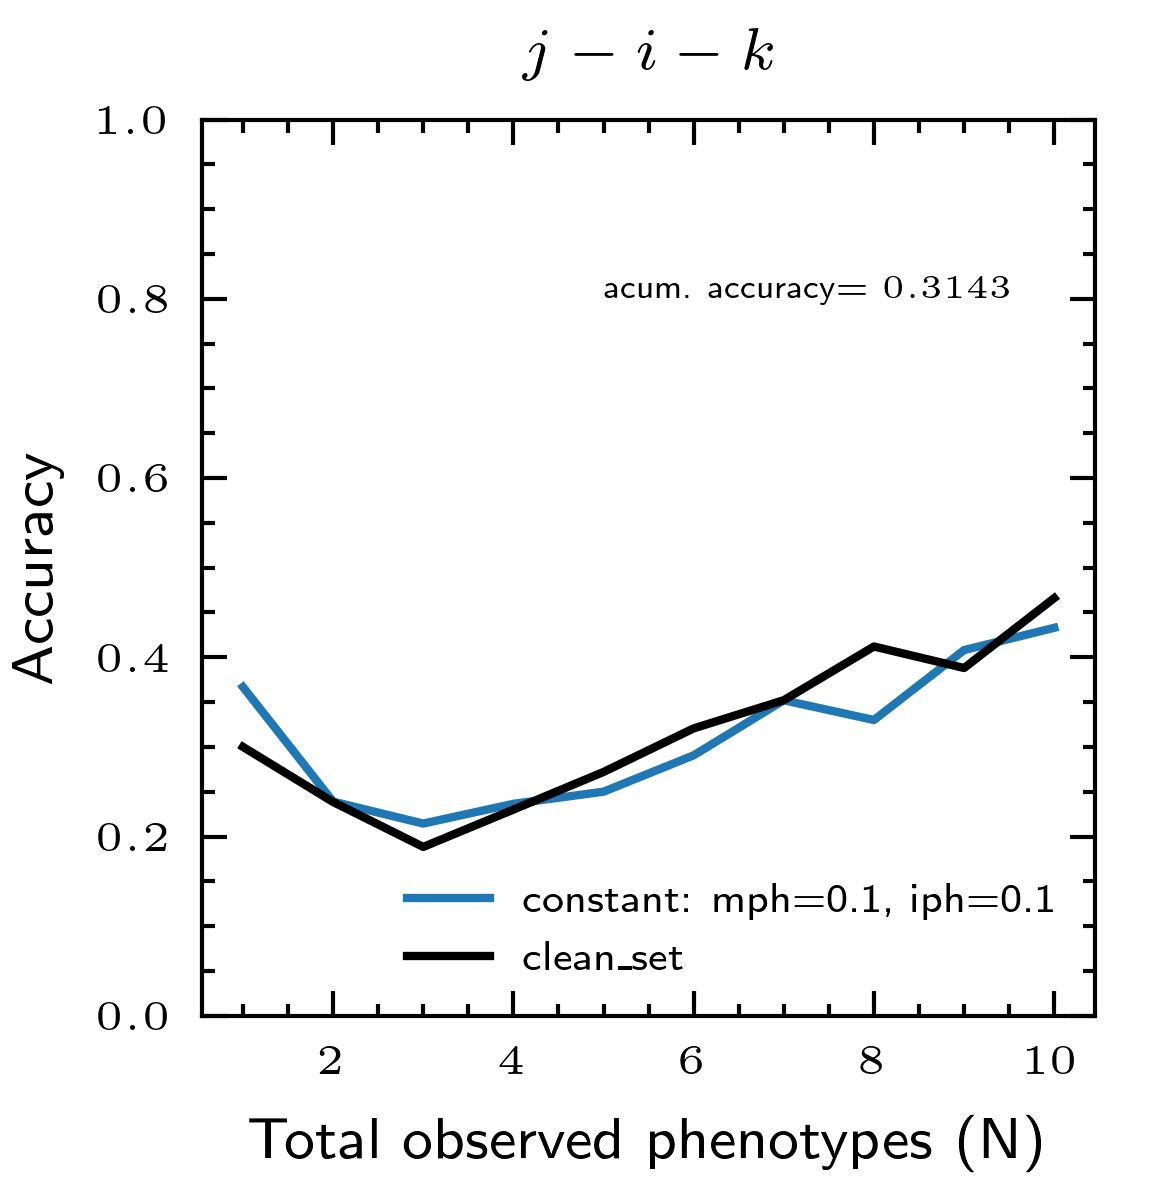
\includegraphics{docs/metrics_evaluation/j-i-k.png} \caption{Caption for docs/metrics_evaluation/j-i-k.png.} \end{figure}
\begin{figure}[h] \centering \includegraphics{docs/metrics_evaluation/j-i.png} \caption{Caption for docs/metrics_evaluation/j-i.png.} \end{figure}
\begin{figure}[h] \centering \includegraphics{docs/metrics_evaluation/j_solo.png} \caption{Caption for docs/metrics_evaluation/j_solo.png.} \end{figure}
\begin{figure}[h] \centering \includegraphics{docs/metrics_evaluation/jsobre1+i+k.png} \caption{Caption for docs/metrics_evaluation/jsobre1+i+k.png.} \end{figure}
\begin{figure}[h] \centering \includegraphics{docs/metrics_evaluation/similaridad_accuracy_exponencial.png} \caption{Caption for docs/metrics_evaluation/similaridad_accuracy_exponencial.png.} \end{figure}
\begin{figure}[h] \centering \includegraphics{docs/metrics_evaluation/similaridad_accuracy_logaritmico.png} \caption{Caption for docs/metrics_evaluation/similaridad_accuracy_logaritmico.png.} \end{figure}
\begin{figure}[h] \centering \includegraphics{docs/metrics_evaluation/similaridad_lineal.png} \caption{Caption for docs/metrics_evaluation/similaridad_lineal.png.} \end{figure}
\begin{figure}[h] \centering \includegraphics{docs/similaridad_accuracy_exponencial.png} \caption{Caption for docs/similaridad_accuracy_exponencial.png.} \end{figure}
\begin{figure}[h] \centering \includegraphics{docs/similaridad_accuracy_logaritmico.png} \caption{Caption for docs/similaridad_accuracy_logaritmico.png.} \end{figure}
\begin{figure}[h] \centering \includegraphics{docs/real_sets_evaluation.png} \caption{Caption for docs/real_sets_evaluation.png.} \end{figure}
\begin{figure}[h] \centering \includegraphics{docs/bipartite_2nd_level.png} \caption{Caption for docs/bipartite_2nd_level.png.} \end{figure}
\begin{figure}[h] \centering \includegraphics{docs/bipartite_gene_disease.png} \caption{Caption for docs/bipartite_gene_disease.png.} \end{figure}
\begin{figure}[h] \centering \includegraphics{docs/clinvar_bitgenia_goldstandard_phenweights.png} \caption{Caption for docs/clinvar_bitgenia_goldstandard_phenweights.png.} \end{figure}
\begin{figure}[h] \centering \includegraphics{docs/disease_network_l2.png} \caption{Caption for docs/disease_network_l2.png.} \end{figure}
\begin{figure}[h] \centering \includegraphics{docs/disease_zoom_top10degree.png} \caption{Caption for docs/disease_zoom_top10degree.png.} \end{figure}
\begin{figure}[h] \centering \includegraphics{docs/espacio_de_parametros_para_comunes.png} \caption{Caption for docs/espacio_de_parametros_para_comunes.png.} \end{figure}
\begin{figure}[h] \centering \includegraphics{docs/espacio_de_parametros_para_normalizadas.png} \caption{Caption for docs/espacio_de_parametros_para_normalizadas.png.} \end{figure}
\begin{figure}[h] \centering \includegraphics{docs/especificidad_de_bitgenia_clinvar_y_goldstandard.png} \caption{Caption for docs/especificidad_de_bitgenia_clinvar_y_goldstandard.png.} \end{figure}
\begin{figure}[h] \centering \includegraphics{docs/freq_aparicion_clinvar_bitgenia_gold_stand.png} \caption{Caption for docs/freq_aparicion_clinvar_bitgenia_gold_stand.png.} \end{figure}
\begin{figure}[h] \centering \includegraphics{docs/gene_network.png} \caption{Caption for docs/gene_network.png.} \end{figure}
\begin{figure}[h] \centering \includegraphics{docs/gene_network_l2.png} \caption{Caption for docs/gene_network_l2.png.} \end{figure}
\begin{figure}[h] \centering \includegraphics{docs/human_disease_network.png} \caption{Caption for docs/human_disease_network.png.} \end{figure}
\begin{figure}[h] \centering \includegraphics{docs/real_sets_evaluation_dif_metrics.png} \caption{Caption for docs/real_sets_evaluation_dif_metrics.png.} \end{figure}
\begin{figure}[h] \centering \includegraphics{docs/red.png} \caption{Caption for docs/red.png.} \end{figure}
\begin{figure}[h] \centering \includegraphics{docs/clinvar_mph&iph.png} \caption{Caption for docs/clinvar_mph&iph.png.} \end{figure}
\begin{figure}[h] \centering \includegraphics{docs/last_version/boxplot_rankings_bitgenia.png} \caption{Caption for docs/last_version/boxplot_rankings_bitgenia.png.} \end{figure}
\begin{figure}[h] \centering \includegraphics{docs/last_version/distancias_distribucion_clinvar.png} \caption{Caption for docs/last_version/distancias_distribucion_clinvar.png.} \end{figure}
\begin{figure}[h] \centering \includegraphics{docs/last_version/recall_at_n_3_features.png} \caption{Caption for docs/last_version/recall_at_n_3_features.png.} \end{figure}
\begin{figure}[h] \centering \includegraphics{docs/resumen_all_in_one.png} \caption{Caption for docs/resumen_all_in_one.png.} \end{figure}
%FiguresEnd
\subsection{Bibliography}
\subsection{Thoughts}

\section{04-06-2023}
\subsection{Commits}
\paragraph{Commit: fcdee47}
Commit Message: agrego la función parametro para probar las nuevas funciones

\paragraph{Commit: 435d42e}
Commit Message: en linear model lab agrego la capacidad de que la funcion model evaluating y la función calculate gene parameters puedan evaluar las nuevas métricas que se dispongan en la función parametro de phen_gen_weight_functions

\paragraph{Commit: 5b2b424}
Commit Message: agrego en el archivo plots.py la función accuracy para medir individualmente cada métrica

\paragraph{Commit: 99088c5}
Commit Message: modifico especificidad del gen poniendo k en logaritmo

\paragraph{Commit: d558a88}
Commit Message: arreglo la definición que había hecho de especificidad porque estaba mal escrita

\paragraph{Commit: e88a0b3}
Commit Message: prueba cambiando especificidad poniendo a k en un exponente de 10

\paragraph{Commit: cba1811}
Commit Message: arreglo algo que al parecer estaba mal en model_evaluating, que me confundí entre las variables n_metrica y nueva_muetrica, que son, dicho sea de paso, bastante inconvenientes los nombres, debería cambiar por otros

\paragraph{Commit: ff87169}
Commit Message: le saco los argumentos definidos de model evaluating y calculate gene parameters

\paragraph{Commit: 627b278}
Commit Message: ahora cambio True y False de nueva métrica por 'si' 'no', a ver si quizás es algo de eso

\paragraph{Commit: b43bb67}
Commit Message: también agrego una 'a' a un 'n_metric' que faltaba

\paragraph{Commit: 8eb196c}
Commit Message: cambio todos los betha por beta en linear model lab

\paragraph{Commit: 02318c3}
Commit Message: SOLUCIONADO. El problema estaba en calculate_gene_parameters, que asignabamos el booleano a nueva_metrica pero después esa variable cambiaba por el parámetro calculado para el gen candidato, ahora lo solucionamos y debería funcionar todo correctamente

\paragraph{Commit: 49694d7}
Commit Message: es decir que lo anterior no funcionaba no porque no calculase los parámetros sino porque no ordenaba el dataframe

\paragraph{Commit: eef3c10}
Commit Message: al parametro 3 de las nuevas métricas lo corrigo para no tener zerodivisionerror

\paragraph{Commit: e4d8092}
Commit Message: a especificidad_del_gen le agrego la feature type_of_func, para luego probar si queremos exponencial, logarítmica o lineal

\paragraph{Commit: dac3246}
Commit Message: todo funcionando. Las pruebas de métricas nuevas van yendo bien y se están descubriendo cosas interesantes. La especificidad descubrimos que la penalización de k tiene que se logarítmica. Queda por ver la similaridad.

\paragraph{Commit: 09addae}
Commit Message: generé todos los gráficos de rendimiento para especificidad similaridad capitalidad y para algunos a parte. A parte para i y k no corrí porque son complementarios de j, no tendría sentido hacerlo

\paragraph{Commit: d743385}
Commit Message: agrego la función accumulated_accuracy para calcular el accuracy acumulado a lo largo de N y así poder elegir cuantitativamente con cuál métrica me quedo

\paragraph{Commit: 90286d2}
Commit Message: dejo especificidad logarítmica, similaridad logarítmica y capitalid logarítmica, que son las que más accuracy acumulado obtuviewron

\paragraph{Commit: 3a1e9e0}
Commit Message: en este punto están todas las combinaciones algebraicas hechas y también todas las combinaciones de a pares de métricas. Conclusión, la similaridad logarítmica sola es la que mejor desempeña hasta ahora. Agregarle métricaslo mantiene igual

\paragraph{Commit: 3a43cc3}
Commit Message: vuelvo a plotear con los labels y títulos más grandes

\paragraph{Commit: 34e653b}
Commit Message: arreglo los sets reales, recuperando los términos hpo originales, para que sea consistente con las funciones anteriormente escritas, y elimino los anteriores

\paragraph{Commit: 8b6ce8d}
Commit Message: en phen_gen_weight functions agrego la propiedad precision en la función fen_reales_del_gen. Cuando es True, me toma de la base de datos exacta, cuando es False, me toma de la base de datos vaga

\paragraph{Commit: ab6f479}
Commit Message: lo mismo que el anterior commit pero debuuggeado

\paragraph{Commit: eba267b}
Commit Message: creo vage_gene_phenotype_dict.json a partir de phenotype_gene_dict

\paragraph{Commit: bea3b8e}
Commit Message: termino de tunear fen_reales_del_gen. Ya está listo para usarse

\paragraph{Commit: d85db3b}
Commit Message: en plots.py ahora también agrego la evaluación de sets reales y su gráfico

\paragraph{Commit: 60f1b2a}
Commit Message: sesión de pruebas en set reales terminada

\paragraph{Commit: f885698}
Commit Message: hago el plot evaluando en set reales con diferentes métricas

\paragraph{Commit: 41c5e56}
Commit Message: agrego las dos métricas que vamos a usar de ahora en más a model_real_evaluating, el top 50 y la media y mediana de rankings

\paragraph{Commit: 1c731da}
Commit Message: plot de espacio de parametros para j, i y k

\paragraph{Commit: a846b8e}
Commit Message: espacio de parámetros para i j y k normalizadas

\paragraph{Commit: 98d1c1c}
Commit Message: plot para el espacio de parámetros de las comunes i j y k

\paragraph{Commit: 698cfb4}
Commit Message: pesos universales de fenotipos

\paragraph{Commit: 61e4da9}
Commit Message: en la función parámetro ahora le agrego los pesos universales de fenotiupos

\paragraph{Commit: da05a08}
Commit Message: código y .csv con propiedades de los fenotipos como nodos: hijos, ancestros, y frecuencia relativa.

\paragraph{Commit: f1728ed}
Commit Message: calculo para clinvar, bitgenia y gold standard de la profundidad de los fenotipos en la forma de media de nodos hijos y nodos ancestros

\paragraph{Commit: 1dfbf10}
Commit Message: agrego también el cálculo de la media de la frecuencia de aparición de cada fenotipo observado en cada base de datos

\paragraph{Commit: 8609fa5}
Commit Message: agrego owl.py, donde vamos a poder explorar muchos más atributos de fenotipos, enfermedades y genes

\paragraph{Commit: a087ad7}
Commit Message: escribo funciones básicas para obtener genes fenotipos y enfermedades de orpha

\paragraph{Commit: dd0bc73}
Commit Message: termino de escribir las funciones que usan los xml de orpha, ahora también tenemos la clasificación más alta para cada enfermedad

\paragraph{Commit: 797aa68}
Commit Message: gene_phenotype_network antes de ser cambiada a gene_disease_network.py

\paragraph{Commit: ef9d645}
Commit Message: plot de la red de enfermedades

\paragraph{Commit: 84fb6f7}
Commit Message: ploteo de la red de genes en nivel 2

\paragraph{Commit: 5ff862d}
Commit Message: ploteo de la red de diseases de nivel 2

\paragraph{Commit: 3d5531e}
Commit Message: agrego la data de orpha, reestrucuro un poco la carpeta data y también se agrega el .py de redes yt algunos gráficos

\paragraph{Commit: bb902ab}
Commit Message: incorporando orpha y funciones modulares. Todo funcionando a la perfección

\paragraph{Commit: 0c0183e}
Commit Message: casos clínicos corregidos

\paragraph{Commit: f7925a6}
Commit Message: sigo refinando el modelo v2 con orpha

\paragraph{Commit: 4b740da}
Commit Message: agrego la función get_average_age_of_onset() que le damos un orphacode y nos devuelve la edad media de aparición de los síntomas

\paragraph{Commit: 89670d7}
Commit Message: agrego how_many_observed() para la simulación de datos

\paragraph{Commit: 5506a79}
Commit Message: single_disease_simulator funcionando

\paragraph{Commit: 5414c3f}
Commit Message: generating_sets con las primeras pruebas de simulaciones

\paragraph{Commit: 791b3c5}
Commit Message: agregando la feature para que elija los síntomas según una distribución de pesos empíricos

\paragraph{Commit: 702c39f}
Commit Message: en set_simulator_utils, agregamos la distribución de pesos empíricos para cada fenotipo simulado en single_disease_simulator

%CommitsEnd
\subsection{Figures}
\begin{figure}[h] \centering \includegraphics{docs/especificidad_accuracy_exponencial.png} \caption{Caption for docs/especificidad_accuracy_exponencial.png.} \end{figure}
\begin{figure}[h] \centering \includegraphics{docs/especificidad_accuracy_logaritmico.png} \caption{Caption for docs/especificidad_accuracy_logaritmico.png.} \end{figure}
\begin{figure}[h] \centering \includegraphics{docs/j-i-k.png} \caption{Caption for docs/j-i-k.png.} \end{figure}
\begin{figure}[h] \centering \includegraphics{docs/j-i.png} \caption{Caption for docs/j-i.png.} \end{figure}
\begin{figure}[h] \centering \includegraphics{docs/jsobre1+i+k.png} \caption{Caption for docs/jsobre1+i+k.png.} \end{figure}
\begin{figure}[h] \centering \includegraphics{docs/capitalidad_accuracy_exponencial.png} \caption{Caption for docs/capitalidad_accuracy_exponencial.png.} \end{figure}
\begin{figure}[h] \centering \includegraphics{docs/capitalidad_accuracy_logaritmico.png} \caption{Caption for docs/capitalidad_accuracy_logaritmico.png.} \end{figure}
\begin{figure}[h] \centering \includegraphics{docs/j_solo.png} \caption{Caption for docs/j_solo.png.} \end{figure}
\begin{figure}[h] \centering \includegraphics{docs/similaridad_accuracy_exponencial.png} \caption{Caption for docs/similaridad_accuracy_exponencial.png.} \end{figure}
\begin{figure}[h] \centering \includegraphics{docs/similaridad_accuracy_logaritmico.png} \caption{Caption for docs/similaridad_accuracy_logaritmico.png.} \end{figure}
\begin{figure}[h] \centering \includegraphics{docs/-i-k.png} \caption{Caption for docs/-i-k.png.} \end{figure}
\begin{figure}[h] \centering \includegraphics{docs/-i_solo.png} \caption{Caption for docs/-i_solo.png.} \end{figure}
\begin{figure}[h] \centering \includegraphics{docs/-k_solo.png} \caption{Caption for docs/-k_solo.png.} \end{figure}
\begin{figure}[h] \centering \includegraphics{docs/cap_mas_esp_mas_sim.png} \caption{Caption for docs/cap_mas_esp_mas_sim.png.} \end{figure}
\begin{figure}[h] \centering \includegraphics{docs/cap_mas_sim.png} \caption{Caption for docs/cap_mas_sim.png.} \end{figure}
\begin{figure}[h] \centering \includegraphics{docs/esp_mas_cap.png} \caption{Caption for docs/esp_mas_cap.png.} \end{figure}
\begin{figure}[h] \centering \includegraphics{docs/esp_mas_sim.png} \caption{Caption for docs/esp_mas_sim.png.} \end{figure}
\begin{figure}[h] \centering \includegraphics{docs/-i-k.png} \caption{Caption for docs/-i-k.png.} \end{figure}
\begin{figure}[h] \centering \includegraphics{docs/-i_solo.png} \caption{Caption for docs/-i_solo.png.} \end{figure}
\begin{figure}[h] \centering \includegraphics{docs/-k_solo.png} \caption{Caption for docs/-k_solo.png.} \end{figure}
\begin{figure}[h] \centering \includegraphics{docs/Accuracy_capitalidad.png} \caption{Caption for docs/Accuracy_capitalidad.png.} \end{figure}
\begin{figure}[h] \centering \includegraphics{docs/Accuracy_especificidad.png} \caption{Caption for docs/Accuracy_especificidad.png.} \end{figure}
\begin{figure}[h] \centering \includegraphics{docs/Accuracy_similaridad.png} \caption{Caption for docs/Accuracy_similaridad.png.} \end{figure}
\begin{figure}[h] \centering \includegraphics{docs/cap_mas_esp_mas_sim.png} \caption{Caption for docs/cap_mas_esp_mas_sim.png.} \end{figure}
\begin{figure}[h] \centering \includegraphics{docs/cap_mas_sim.png} \caption{Caption for docs/cap_mas_sim.png.} \end{figure}
\begin{figure}[h] \centering \includegraphics{docs/capitalidad_accuracy_exponencial.png} \caption{Caption for docs/capitalidad_accuracy_exponencial.png.} \end{figure}
\begin{figure}[h] \centering \includegraphics{docs/capitalidad_accuracy_logaritmico.png} \caption{Caption for docs/capitalidad_accuracy_logaritmico.png.} \end{figure}
\begin{figure}[h] \centering \includegraphics{docs/esp_mas_cap.png} \caption{Caption for docs/esp_mas_cap.png.} \end{figure}
\begin{figure}[h] \centering \includegraphics{docs/esp_mas_sim.png} \caption{Caption for docs/esp_mas_sim.png.} \end{figure}
\begin{figure}[h] \centering \includegraphics{docs/especificidad_accuracy_exponencial.png} \caption{Caption for docs/especificidad_accuracy_exponencial.png.} \end{figure}
\begin{figure}[h] \centering \includegraphics{docs/especificidad_accuracy_logaritmico.png} \caption{Caption for docs/especificidad_accuracy_logaritmico.png.} \end{figure}
\begin{figure}[h] \centering \includegraphics{docs/j-i-k.png} \caption{Caption for docs/j-i-k.png.} \end{figure}
\begin{figure}[h] \centering \includegraphics{docs/j-i.png} \caption{Caption for docs/j-i.png.} \end{figure}
\begin{figure}[h] \centering \includegraphics{docs/j_solo.png} \caption{Caption for docs/j_solo.png.} \end{figure}
\begin{figure}[h] \centering \includegraphics{docs/jsobre1+i+k.png} \caption{Caption for docs/jsobre1+i+k.png.} \end{figure}
\begin{figure}[h] \centering \includegraphics{docs/metrics_evaluation/-i-k.png} \caption{Caption for docs/metrics_evaluation/-i-k.png.} \end{figure}
\begin{figure}[h] \centering \includegraphics{docs/metrics_evaluation/-i_solo.png} \caption{Caption for docs/metrics_evaluation/-i_solo.png.} \end{figure}
\begin{figure}[h] \centering \includegraphics{docs/metrics_evaluation/-k_solo.png} \caption{Caption for docs/metrics_evaluation/-k_solo.png.} \end{figure}
\begin{figure}[h] \centering \includegraphics{docs/metrics_evaluation/cap_mas_esp_mas_sim.png} \caption{Caption for docs/metrics_evaluation/cap_mas_esp_mas_sim.png.} \end{figure}
\begin{figure}[h] \centering \includegraphics{docs/metrics_evaluation/cap_mas_sim.png} \caption{Caption for docs/metrics_evaluation/cap_mas_sim.png.} \end{figure}
\begin{figure}[h] \centering \includegraphics{docs/metrics_evaluation/capitalidad_accuracy_exponencial.png} \caption{Caption for docs/metrics_evaluation/capitalidad_accuracy_exponencial.png.} \end{figure}
\begin{figure}[h] \centering \includegraphics{docs/metrics_evaluation/capitalidad_accuracy_lineal.png} \caption{Caption for docs/metrics_evaluation/capitalidad_accuracy_lineal.png.} \end{figure}
\begin{figure}[h] \centering \includegraphics{docs/metrics_evaluation/capitalidad_accuracy_logaritmico.png} \caption{Caption for docs/metrics_evaluation/capitalidad_accuracy_logaritmico.png.} \end{figure}
\begin{figure}[h] \centering \includegraphics{docs/metrics_evaluation/esp_mas_cap.png} \caption{Caption for docs/metrics_evaluation/esp_mas_cap.png.} \end{figure}
\begin{figure}[h] \centering \includegraphics{docs/metrics_evaluation/esp_mas_sim.png} \caption{Caption for docs/metrics_evaluation/esp_mas_sim.png.} \end{figure}
\begin{figure}[h] \centering \includegraphics{docs/metrics_evaluation/especificidad_accuracy_exponencial.png} \caption{Caption for docs/metrics_evaluation/especificidad_accuracy_exponencial.png.} \end{figure}
\begin{figure}[h] \centering \includegraphics{docs/metrics_evaluation/especificidad_accuracy_lineal.png} \caption{Caption for docs/metrics_evaluation/especificidad_accuracy_lineal.png.} \end{figure}
\begin{figure}[h] \centering \includegraphics{docs/metrics_evaluation/especificidad_accuracy_logaritmico.png} \caption{Caption for docs/metrics_evaluation/especificidad_accuracy_logaritmico.png.} \end{figure}
\begin{figure}[h] \centering \includegraphics{docs/metrics_evaluation/j-i-k.png} \caption{Caption for docs/metrics_evaluation/j-i-k.png.} \end{figure}
\begin{figure}[h] \centering \includegraphics{docs/metrics_evaluation/j-i.png} \caption{Caption for docs/metrics_evaluation/j-i.png.} \end{figure}
\begin{figure}[h] \centering \includegraphics{docs/metrics_evaluation/j_solo.png} \caption{Caption for docs/metrics_evaluation/j_solo.png.} \end{figure}
\begin{figure}[h] \centering \includegraphics{docs/metrics_evaluation/jsobre1+i+k.png} \caption{Caption for docs/metrics_evaluation/jsobre1+i+k.png.} \end{figure}
\begin{figure}[h] \centering \includegraphics{docs/metrics_evaluation/similaridad_accuracy_exponencial.png} \caption{Caption for docs/metrics_evaluation/similaridad_accuracy_exponencial.png.} \end{figure}
\begin{figure}[h] \centering \includegraphics{docs/metrics_evaluation/similaridad_accuracy_logaritmico.png} \caption{Caption for docs/metrics_evaluation/similaridad_accuracy_logaritmico.png.} \end{figure}
\begin{figure}[h] \centering \includegraphics{docs/metrics_evaluation/similaridad_lineal.png} \caption{Caption for docs/metrics_evaluation/similaridad_lineal.png.} \end{figure}
\begin{figure}[h] \centering \includegraphics{docs/similaridad_accuracy_exponencial.png} \caption{Caption for docs/similaridad_accuracy_exponencial.png.} \end{figure}
\begin{figure}[h] \centering \includegraphics{docs/similaridad_accuracy_logaritmico.png} \caption{Caption for docs/similaridad_accuracy_logaritmico.png.} \end{figure}
\begin{figure}[h] \centering \includegraphics{docs/real_sets_evaluation.png} \caption{Caption for docs/real_sets_evaluation.png.} \end{figure}
\begin{figure}[h] \centering \includegraphics{docs/bipartite_2nd_level.png} \caption{Caption for docs/bipartite_2nd_level.png.} \end{figure}
\begin{figure}[h] \centering \includegraphics{docs/bipartite_gene_disease.png} \caption{Caption for docs/bipartite_gene_disease.png.} \end{figure}
\begin{figure}[h] \centering \includegraphics{docs/clinvar_bitgenia_goldstandard_phenweights.png} \caption{Caption for docs/clinvar_bitgenia_goldstandard_phenweights.png.} \end{figure}
\begin{figure}[h] \centering \includegraphics{docs/disease_network_l2.png} \caption{Caption for docs/disease_network_l2.png.} \end{figure}
\begin{figure}[h] \centering \includegraphics{docs/disease_zoom_top10degree.png} \caption{Caption for docs/disease_zoom_top10degree.png.} \end{figure}
\begin{figure}[h] \centering \includegraphics{docs/espacio_de_parametros_para_comunes.png} \caption{Caption for docs/espacio_de_parametros_para_comunes.png.} \end{figure}
\begin{figure}[h] \centering \includegraphics{docs/espacio_de_parametros_para_normalizadas.png} \caption{Caption for docs/espacio_de_parametros_para_normalizadas.png.} \end{figure}
\begin{figure}[h] \centering \includegraphics{docs/especificidad_de_bitgenia_clinvar_y_goldstandard.png} \caption{Caption for docs/especificidad_de_bitgenia_clinvar_y_goldstandard.png.} \end{figure}
\begin{figure}[h] \centering \includegraphics{docs/freq_aparicion_clinvar_bitgenia_gold_stand.png} \caption{Caption for docs/freq_aparicion_clinvar_bitgenia_gold_stand.png.} \end{figure}
\begin{figure}[h] \centering \includegraphics{docs/gene_network.png} \caption{Caption for docs/gene_network.png.} \end{figure}
\begin{figure}[h] \centering \includegraphics{docs/gene_network_l2.png} \caption{Caption for docs/gene_network_l2.png.} \end{figure}
\begin{figure}[h] \centering \includegraphics{docs/human_disease_network.png} \caption{Caption for docs/human_disease_network.png.} \end{figure}
\begin{figure}[h] \centering \includegraphics{docs/real_sets_evaluation_dif_metrics.png} \caption{Caption for docs/real_sets_evaluation_dif_metrics.png.} \end{figure}
\begin{figure}[h] \centering \includegraphics{docs/red.png} \caption{Caption for docs/red.png.} \end{figure}
\begin{figure}[h] \centering \includegraphics{docs/clinvar_mph&iph.png} \caption{Caption for docs/clinvar_mph&iph.png.} \end{figure}
\begin{figure}[h] \centering \includegraphics{docs/last_version/boxplot_rankings_bitgenia.png} \caption{Caption for docs/last_version/boxplot_rankings_bitgenia.png.} \end{figure}
\begin{figure}[h] \centering \includegraphics{docs/last_version/distancias_distribucion_clinvar.png} \caption{Caption for docs/last_version/distancias_distribucion_clinvar.png.} \end{figure}
\begin{figure}[h] \centering \includegraphics{docs/last_version/recall_at_n_3_features.png} \caption{Caption for docs/last_version/recall_at_n_3_features.png.} \end{figure}
\begin{figure}[h] \centering \includegraphics{docs/resumen_all_in_one.png} \caption{Caption for docs/resumen_all_in_one.png.} \end{figure}
%FiguresEnd
\subsection{Bibliography}
\subsection{Thoughts}

\section{05-06-2023}
\subsection{Commits}
\paragraph{Commit: e88a0b3}
Commit Message: prueba cambiando especificidad poniendo a k en un exponente de 10

\paragraph{Commit: cba1811}
Commit Message: arreglo algo que al parecer estaba mal en model_evaluating, que me confundí entre las variables n_metrica y nueva_muetrica, que son, dicho sea de paso, bastante inconvenientes los nombres, debería cambiar por otros

\paragraph{Commit: ff87169}
Commit Message: le saco los argumentos definidos de model evaluating y calculate gene parameters

\paragraph{Commit: 627b278}
Commit Message: ahora cambio True y False de nueva métrica por 'si' 'no', a ver si quizás es algo de eso

\paragraph{Commit: b43bb67}
Commit Message: también agrego una 'a' a un 'n_metric' que faltaba

\paragraph{Commit: 8eb196c}
Commit Message: cambio todos los betha por beta en linear model lab

\paragraph{Commit: 02318c3}
Commit Message: SOLUCIONADO. El problema estaba en calculate_gene_parameters, que asignabamos el booleano a nueva_metrica pero después esa variable cambiaba por el parámetro calculado para el gen candidato, ahora lo solucionamos y debería funcionar todo correctamente

\paragraph{Commit: 49694d7}
Commit Message: es decir que lo anterior no funcionaba no porque no calculase los parámetros sino porque no ordenaba el dataframe

\paragraph{Commit: eef3c10}
Commit Message: al parametro 3 de las nuevas métricas lo corrigo para no tener zerodivisionerror

\paragraph{Commit: e4d8092}
Commit Message: a especificidad_del_gen le agrego la feature type_of_func, para luego probar si queremos exponencial, logarítmica o lineal

\paragraph{Commit: dac3246}
Commit Message: todo funcionando. Las pruebas de métricas nuevas van yendo bien y se están descubriendo cosas interesantes. La especificidad descubrimos que la penalización de k tiene que se logarítmica. Queda por ver la similaridad.

\paragraph{Commit: 09addae}
Commit Message: generé todos los gráficos de rendimiento para especificidad similaridad capitalidad y para algunos a parte. A parte para i y k no corrí porque son complementarios de j, no tendría sentido hacerlo

\paragraph{Commit: d743385}
Commit Message: agrego la función accumulated_accuracy para calcular el accuracy acumulado a lo largo de N y así poder elegir cuantitativamente con cuál métrica me quedo

\paragraph{Commit: 90286d2}
Commit Message: dejo especificidad logarítmica, similaridad logarítmica y capitalid logarítmica, que son las que más accuracy acumulado obtuviewron

\paragraph{Commit: 3a1e9e0}
Commit Message: en este punto están todas las combinaciones algebraicas hechas y también todas las combinaciones de a pares de métricas. Conclusión, la similaridad logarítmica sola es la que mejor desempeña hasta ahora. Agregarle métricaslo mantiene igual

\paragraph{Commit: 3a43cc3}
Commit Message: vuelvo a plotear con los labels y títulos más grandes

\paragraph{Commit: 34e653b}
Commit Message: arreglo los sets reales, recuperando los términos hpo originales, para que sea consistente con las funciones anteriormente escritas, y elimino los anteriores

\paragraph{Commit: 8b6ce8d}
Commit Message: en phen_gen_weight functions agrego la propiedad precision en la función fen_reales_del_gen. Cuando es True, me toma de la base de datos exacta, cuando es False, me toma de la base de datos vaga

\paragraph{Commit: ab6f479}
Commit Message: lo mismo que el anterior commit pero debuuggeado

\paragraph{Commit: eba267b}
Commit Message: creo vage_gene_phenotype_dict.json a partir de phenotype_gene_dict

\paragraph{Commit: bea3b8e}
Commit Message: termino de tunear fen_reales_del_gen. Ya está listo para usarse

\paragraph{Commit: d85db3b}
Commit Message: en plots.py ahora también agrego la evaluación de sets reales y su gráfico

\paragraph{Commit: 60f1b2a}
Commit Message: sesión de pruebas en set reales terminada

\paragraph{Commit: f885698}
Commit Message: hago el plot evaluando en set reales con diferentes métricas

\paragraph{Commit: 41c5e56}
Commit Message: agrego las dos métricas que vamos a usar de ahora en más a model_real_evaluating, el top 50 y la media y mediana de rankings

\paragraph{Commit: 1c731da}
Commit Message: plot de espacio de parametros para j, i y k

\paragraph{Commit: a846b8e}
Commit Message: espacio de parámetros para i j y k normalizadas

\paragraph{Commit: 98d1c1c}
Commit Message: plot para el espacio de parámetros de las comunes i j y k

\paragraph{Commit: 698cfb4}
Commit Message: pesos universales de fenotipos

\paragraph{Commit: 61e4da9}
Commit Message: en la función parámetro ahora le agrego los pesos universales de fenotiupos

\paragraph{Commit: da05a08}
Commit Message: código y .csv con propiedades de los fenotipos como nodos: hijos, ancestros, y frecuencia relativa.

\paragraph{Commit: f1728ed}
Commit Message: calculo para clinvar, bitgenia y gold standard de la profundidad de los fenotipos en la forma de media de nodos hijos y nodos ancestros

\paragraph{Commit: 1dfbf10}
Commit Message: agrego también el cálculo de la media de la frecuencia de aparición de cada fenotipo observado en cada base de datos

\paragraph{Commit: 8609fa5}
Commit Message: agrego owl.py, donde vamos a poder explorar muchos más atributos de fenotipos, enfermedades y genes

\paragraph{Commit: a087ad7}
Commit Message: escribo funciones básicas para obtener genes fenotipos y enfermedades de orpha

\paragraph{Commit: dd0bc73}
Commit Message: termino de escribir las funciones que usan los xml de orpha, ahora también tenemos la clasificación más alta para cada enfermedad

\paragraph{Commit: 797aa68}
Commit Message: gene_phenotype_network antes de ser cambiada a gene_disease_network.py

\paragraph{Commit: ef9d645}
Commit Message: plot de la red de enfermedades

\paragraph{Commit: 84fb6f7}
Commit Message: ploteo de la red de genes en nivel 2

\paragraph{Commit: 5ff862d}
Commit Message: ploteo de la red de diseases de nivel 2

\paragraph{Commit: 3d5531e}
Commit Message: agrego la data de orpha, reestrucuro un poco la carpeta data y también se agrega el .py de redes yt algunos gráficos

\paragraph{Commit: bb902ab}
Commit Message: incorporando orpha y funciones modulares. Todo funcionando a la perfección

\paragraph{Commit: 0c0183e}
Commit Message: casos clínicos corregidos

\paragraph{Commit: f7925a6}
Commit Message: sigo refinando el modelo v2 con orpha

\paragraph{Commit: 4b740da}
Commit Message: agrego la función get_average_age_of_onset() que le damos un orphacode y nos devuelve la edad media de aparición de los síntomas

\paragraph{Commit: 89670d7}
Commit Message: agrego how_many_observed() para la simulación de datos

\paragraph{Commit: 5506a79}
Commit Message: single_disease_simulator funcionando

\paragraph{Commit: 5414c3f}
Commit Message: generating_sets con las primeras pruebas de simulaciones

\paragraph{Commit: 791b3c5}
Commit Message: agregando la feature para que elija los síntomas según una distribución de pesos empíricos

\paragraph{Commit: 702c39f}
Commit Message: en set_simulator_utils, agregamos la distribución de pesos empíricos para cada fenotipo simulado en single_disease_simulator

%CommitsEnd
\subsection{Figures}
\begin{figure}[h] \centering \includegraphics{docs/especificidad_accuracy_exponencial.png} \caption{Caption for docs/especificidad_accuracy_exponencial.png.} \end{figure}
\begin{figure}[h] \centering \includegraphics{docs/especificidad_accuracy_logaritmico.png} \caption{Caption for docs/especificidad_accuracy_logaritmico.png.} \end{figure}
\begin{figure}[h] \centering \includegraphics{docs/j-i-k.png} \caption{Caption for docs/j-i-k.png.} \end{figure}
\begin{figure}[h] \centering \includegraphics{docs/j-i.png} \caption{Caption for docs/j-i.png.} \end{figure}
\begin{figure}[h] \centering \includegraphics{docs/jsobre1+i+k.png} \caption{Caption for docs/jsobre1+i+k.png.} \end{figure}
\begin{figure}[h] \centering \includegraphics{docs/capitalidad_accuracy_exponencial.png} \caption{Caption for docs/capitalidad_accuracy_exponencial.png.} \end{figure}
\begin{figure}[h] \centering \includegraphics{docs/capitalidad_accuracy_logaritmico.png} \caption{Caption for docs/capitalidad_accuracy_logaritmico.png.} \end{figure}
\begin{figure}[h] \centering \includegraphics{docs/j_solo.png} \caption{Caption for docs/j_solo.png.} \end{figure}
\begin{figure}[h] \centering \includegraphics{docs/similaridad_accuracy_exponencial.png} \caption{Caption for docs/similaridad_accuracy_exponencial.png.} \end{figure}
\begin{figure}[h] \centering \includegraphics{docs/similaridad_accuracy_logaritmico.png} \caption{Caption for docs/similaridad_accuracy_logaritmico.png.} \end{figure}
\begin{figure}[h] \centering \includegraphics{docs/-i-k.png} \caption{Caption for docs/-i-k.png.} \end{figure}
\begin{figure}[h] \centering \includegraphics{docs/-i_solo.png} \caption{Caption for docs/-i_solo.png.} \end{figure}
\begin{figure}[h] \centering \includegraphics{docs/-k_solo.png} \caption{Caption for docs/-k_solo.png.} \end{figure}
\begin{figure}[h] \centering \includegraphics{docs/cap_mas_esp_mas_sim.png} \caption{Caption for docs/cap_mas_esp_mas_sim.png.} \end{figure}
\begin{figure}[h] \centering \includegraphics{docs/cap_mas_sim.png} \caption{Caption for docs/cap_mas_sim.png.} \end{figure}
\begin{figure}[h] \centering \includegraphics{docs/esp_mas_cap.png} \caption{Caption for docs/esp_mas_cap.png.} \end{figure}
\begin{figure}[h] \centering \includegraphics{docs/esp_mas_sim.png} \caption{Caption for docs/esp_mas_sim.png.} \end{figure}
\begin{figure}[h] \centering \includegraphics{docs/-i-k.png} \caption{Caption for docs/-i-k.png.} \end{figure}
\begin{figure}[h] \centering \includegraphics{docs/-i_solo.png} \caption{Caption for docs/-i_solo.png.} \end{figure}
\begin{figure}[h] \centering \includegraphics{docs/-k_solo.png} \caption{Caption for docs/-k_solo.png.} \end{figure}
\begin{figure}[h] \centering \includegraphics{docs/Accuracy_capitalidad.png} \caption{Caption for docs/Accuracy_capitalidad.png.} \end{figure}
\begin{figure}[h] \centering \includegraphics{docs/Accuracy_especificidad.png} \caption{Caption for docs/Accuracy_especificidad.png.} \end{figure}
\begin{figure}[h] \centering \includegraphics{docs/Accuracy_similaridad.png} \caption{Caption for docs/Accuracy_similaridad.png.} \end{figure}
\begin{figure}[h] \centering \includegraphics{docs/cap_mas_esp_mas_sim.png} \caption{Caption for docs/cap_mas_esp_mas_sim.png.} \end{figure}
\begin{figure}[h] \centering \includegraphics{docs/cap_mas_sim.png} \caption{Caption for docs/cap_mas_sim.png.} \end{figure}
\begin{figure}[h] \centering \includegraphics{docs/capitalidad_accuracy_exponencial.png} \caption{Caption for docs/capitalidad_accuracy_exponencial.png.} \end{figure}
\begin{figure}[h] \centering \includegraphics{docs/capitalidad_accuracy_logaritmico.png} \caption{Caption for docs/capitalidad_accuracy_logaritmico.png.} \end{figure}
\begin{figure}[h] \centering \includegraphics{docs/esp_mas_cap.png} \caption{Caption for docs/esp_mas_cap.png.} \end{figure}
\begin{figure}[h] \centering \includegraphics{docs/esp_mas_sim.png} \caption{Caption for docs/esp_mas_sim.png.} \end{figure}
\begin{figure}[h] \centering \includegraphics{docs/especificidad_accuracy_exponencial.png} \caption{Caption for docs/especificidad_accuracy_exponencial.png.} \end{figure}
\begin{figure}[h] \centering \includegraphics{docs/especificidad_accuracy_logaritmico.png} \caption{Caption for docs/especificidad_accuracy_logaritmico.png.} \end{figure}
\begin{figure}[h] \centering \includegraphics{docs/j-i-k.png} \caption{Caption for docs/j-i-k.png.} \end{figure}
\begin{figure}[h] \centering \includegraphics{docs/j-i.png} \caption{Caption for docs/j-i.png.} \end{figure}
\begin{figure}[h] \centering \includegraphics{docs/j_solo.png} \caption{Caption for docs/j_solo.png.} \end{figure}
\begin{figure}[h] \centering \includegraphics{docs/jsobre1+i+k.png} \caption{Caption for docs/jsobre1+i+k.png.} \end{figure}
\begin{figure}[h] \centering \includegraphics{docs/metrics_evaluation/-i-k.png} \caption{Caption for docs/metrics_evaluation/-i-k.png.} \end{figure}
\begin{figure}[h] \centering \includegraphics{docs/metrics_evaluation/-i_solo.png} \caption{Caption for docs/metrics_evaluation/-i_solo.png.} \end{figure}
\begin{figure}[h] \centering \includegraphics{docs/metrics_evaluation/-k_solo.png} \caption{Caption for docs/metrics_evaluation/-k_solo.png.} \end{figure}
\begin{figure}[h] \centering \includegraphics{docs/metrics_evaluation/cap_mas_esp_mas_sim.png} \caption{Caption for docs/metrics_evaluation/cap_mas_esp_mas_sim.png.} \end{figure}
\begin{figure}[h] \centering \includegraphics{docs/metrics_evaluation/cap_mas_sim.png} \caption{Caption for docs/metrics_evaluation/cap_mas_sim.png.} \end{figure}
\begin{figure}[h] \centering \includegraphics{docs/metrics_evaluation/capitalidad_accuracy_exponencial.png} \caption{Caption for docs/metrics_evaluation/capitalidad_accuracy_exponencial.png.} \end{figure}
\begin{figure}[h] \centering \includegraphics{docs/metrics_evaluation/capitalidad_accuracy_lineal.png} \caption{Caption for docs/metrics_evaluation/capitalidad_accuracy_lineal.png.} \end{figure}
\begin{figure}[h] \centering \includegraphics{docs/metrics_evaluation/capitalidad_accuracy_logaritmico.png} \caption{Caption for docs/metrics_evaluation/capitalidad_accuracy_logaritmico.png.} \end{figure}
\begin{figure}[h] \centering \includegraphics{docs/metrics_evaluation/esp_mas_cap.png} \caption{Caption for docs/metrics_evaluation/esp_mas_cap.png.} \end{figure}
\begin{figure}[h] \centering \includegraphics{docs/metrics_evaluation/esp_mas_sim.png} \caption{Caption for docs/metrics_evaluation/esp_mas_sim.png.} \end{figure}
\begin{figure}[h] \centering \includegraphics{docs/metrics_evaluation/especificidad_accuracy_exponencial.png} \caption{Caption for docs/metrics_evaluation/especificidad_accuracy_exponencial.png.} \end{figure}
\begin{figure}[h] \centering \includegraphics{docs/metrics_evaluation/especificidad_accuracy_lineal.png} \caption{Caption for docs/metrics_evaluation/especificidad_accuracy_lineal.png.} \end{figure}
\begin{figure}[h] \centering \includegraphics{docs/metrics_evaluation/especificidad_accuracy_logaritmico.png} \caption{Caption for docs/metrics_evaluation/especificidad_accuracy_logaritmico.png.} \end{figure}
\begin{figure}[h] \centering \includegraphics{docs/metrics_evaluation/j-i-k.png} \caption{Caption for docs/metrics_evaluation/j-i-k.png.} \end{figure}
\begin{figure}[h] \centering \includegraphics{docs/metrics_evaluation/j-i.png} \caption{Caption for docs/metrics_evaluation/j-i.png.} \end{figure}
\begin{figure}[h] \centering \includegraphics{docs/metrics_evaluation/j_solo.png} \caption{Caption for docs/metrics_evaluation/j_solo.png.} \end{figure}
\begin{figure}[h] \centering \includegraphics{docs/metrics_evaluation/jsobre1+i+k.png} \caption{Caption for docs/metrics_evaluation/jsobre1+i+k.png.} \end{figure}
\begin{figure}[h] \centering \includegraphics{docs/metrics_evaluation/similaridad_accuracy_exponencial.png} \caption{Caption for docs/metrics_evaluation/similaridad_accuracy_exponencial.png.} \end{figure}
\begin{figure}[h] \centering \includegraphics{docs/metrics_evaluation/similaridad_accuracy_logaritmico.png} \caption{Caption for docs/metrics_evaluation/similaridad_accuracy_logaritmico.png.} \end{figure}
\begin{figure}[h] \centering \includegraphics{docs/metrics_evaluation/similaridad_lineal.png} \caption{Caption for docs/metrics_evaluation/similaridad_lineal.png.} \end{figure}
\begin{figure}[h] \centering \includegraphics{docs/similaridad_accuracy_exponencial.png} \caption{Caption for docs/similaridad_accuracy_exponencial.png.} \end{figure}
\begin{figure}[h] \centering \includegraphics{docs/similaridad_accuracy_logaritmico.png} \caption{Caption for docs/similaridad_accuracy_logaritmico.png.} \end{figure}
\begin{figure}[h] \centering \includegraphics{docs/real_sets_evaluation.png} \caption{Caption for docs/real_sets_evaluation.png.} \end{figure}
\begin{figure}[h] \centering \includegraphics{docs/bipartite_2nd_level.png} \caption{Caption for docs/bipartite_2nd_level.png.} \end{figure}
\begin{figure}[h] \centering \includegraphics{docs/bipartite_gene_disease.png} \caption{Caption for docs/bipartite_gene_disease.png.} \end{figure}
\begin{figure}[h] \centering \includegraphics{docs/clinvar_bitgenia_goldstandard_phenweights.png} \caption{Caption for docs/clinvar_bitgenia_goldstandard_phenweights.png.} \end{figure}
\begin{figure}[h] \centering \includegraphics{docs/disease_network_l2.png} \caption{Caption for docs/disease_network_l2.png.} \end{figure}
\begin{figure}[h] \centering \includegraphics{docs/disease_zoom_top10degree.png} \caption{Caption for docs/disease_zoom_top10degree.png.} \end{figure}
\begin{figure}[h] \centering \includegraphics{docs/espacio_de_parametros_para_comunes.png} \caption{Caption for docs/espacio_de_parametros_para_comunes.png.} \end{figure}
\begin{figure}[h] \centering \includegraphics{docs/espacio_de_parametros_para_normalizadas.png} \caption{Caption for docs/espacio_de_parametros_para_normalizadas.png.} \end{figure}
\begin{figure}[h] \centering \includegraphics{docs/especificidad_de_bitgenia_clinvar_y_goldstandard.png} \caption{Caption for docs/especificidad_de_bitgenia_clinvar_y_goldstandard.png.} \end{figure}
\begin{figure}[h] \centering \includegraphics{docs/freq_aparicion_clinvar_bitgenia_gold_stand.png} \caption{Caption for docs/freq_aparicion_clinvar_bitgenia_gold_stand.png.} \end{figure}
\begin{figure}[h] \centering \includegraphics{docs/gene_network.png} \caption{Caption for docs/gene_network.png.} \end{figure}
\begin{figure}[h] \centering \includegraphics{docs/gene_network_l2.png} \caption{Caption for docs/gene_network_l2.png.} \end{figure}
\begin{figure}[h] \centering \includegraphics{docs/human_disease_network.png} \caption{Caption for docs/human_disease_network.png.} \end{figure}
\begin{figure}[h] \centering \includegraphics{docs/real_sets_evaluation_dif_metrics.png} \caption{Caption for docs/real_sets_evaluation_dif_metrics.png.} \end{figure}
\begin{figure}[h] \centering \includegraphics{docs/red.png} \caption{Caption for docs/red.png.} \end{figure}
\begin{figure}[h] \centering \includegraphics{docs/clinvar_mph&iph.png} \caption{Caption for docs/clinvar_mph&iph.png.} \end{figure}
\begin{figure}[h] \centering \includegraphics{docs/last_version/boxplot_rankings_bitgenia.png} \caption{Caption for docs/last_version/boxplot_rankings_bitgenia.png.} \end{figure}
\begin{figure}[h] \centering \includegraphics{docs/last_version/distancias_distribucion_clinvar.png} \caption{Caption for docs/last_version/distancias_distribucion_clinvar.png.} \end{figure}
\begin{figure}[h] \centering \includegraphics{docs/last_version/recall_at_n_3_features.png} \caption{Caption for docs/last_version/recall_at_n_3_features.png.} \end{figure}
\begin{figure}[h] \centering \includegraphics{docs/resumen_all_in_one.png} \caption{Caption for docs/resumen_all_in_one.png.} \end{figure}
%FiguresEnd
\subsection{Bibliography}
\subsection{Thoughts}

\section{06-06-2023}
\subsection{Commits}
\paragraph{Commit: d743385}
Commit Message: agrego la función accumulated_accuracy para calcular el accuracy acumulado a lo largo de N y así poder elegir cuantitativamente con cuál métrica me quedo

\paragraph{Commit: 90286d2}
Commit Message: dejo especificidad logarítmica, similaridad logarítmica y capitalid logarítmica, que son las que más accuracy acumulado obtuviewron

\paragraph{Commit: 3a1e9e0}
Commit Message: en este punto están todas las combinaciones algebraicas hechas y también todas las combinaciones de a pares de métricas. Conclusión, la similaridad logarítmica sola es la que mejor desempeña hasta ahora. Agregarle métricaslo mantiene igual

\paragraph{Commit: 3a43cc3}
Commit Message: vuelvo a plotear con los labels y títulos más grandes

\paragraph{Commit: 34e653b}
Commit Message: arreglo los sets reales, recuperando los términos hpo originales, para que sea consistente con las funciones anteriormente escritas, y elimino los anteriores

\paragraph{Commit: 8b6ce8d}
Commit Message: en phen_gen_weight functions agrego la propiedad precision en la función fen_reales_del_gen. Cuando es True, me toma de la base de datos exacta, cuando es False, me toma de la base de datos vaga

\paragraph{Commit: ab6f479}
Commit Message: lo mismo que el anterior commit pero debuuggeado

\paragraph{Commit: eba267b}
Commit Message: creo vage_gene_phenotype_dict.json a partir de phenotype_gene_dict

\paragraph{Commit: bea3b8e}
Commit Message: termino de tunear fen_reales_del_gen. Ya está listo para usarse

\paragraph{Commit: d85db3b}
Commit Message: en plots.py ahora también agrego la evaluación de sets reales y su gráfico

\paragraph{Commit: 60f1b2a}
Commit Message: sesión de pruebas en set reales terminada

\paragraph{Commit: f885698}
Commit Message: hago el plot evaluando en set reales con diferentes métricas

\paragraph{Commit: 41c5e56}
Commit Message: agrego las dos métricas que vamos a usar de ahora en más a model_real_evaluating, el top 50 y la media y mediana de rankings

\paragraph{Commit: 1c731da}
Commit Message: plot de espacio de parametros para j, i y k

\paragraph{Commit: a846b8e}
Commit Message: espacio de parámetros para i j y k normalizadas

\paragraph{Commit: 98d1c1c}
Commit Message: plot para el espacio de parámetros de las comunes i j y k

\paragraph{Commit: 698cfb4}
Commit Message: pesos universales de fenotipos

\paragraph{Commit: 61e4da9}
Commit Message: en la función parámetro ahora le agrego los pesos universales de fenotiupos

\paragraph{Commit: da05a08}
Commit Message: código y .csv con propiedades de los fenotipos como nodos: hijos, ancestros, y frecuencia relativa.

\paragraph{Commit: f1728ed}
Commit Message: calculo para clinvar, bitgenia y gold standard de la profundidad de los fenotipos en la forma de media de nodos hijos y nodos ancestros

\paragraph{Commit: 1dfbf10}
Commit Message: agrego también el cálculo de la media de la frecuencia de aparición de cada fenotipo observado en cada base de datos

\paragraph{Commit: 8609fa5}
Commit Message: agrego owl.py, donde vamos a poder explorar muchos más atributos de fenotipos, enfermedades y genes

\paragraph{Commit: a087ad7}
Commit Message: escribo funciones básicas para obtener genes fenotipos y enfermedades de orpha

\paragraph{Commit: dd0bc73}
Commit Message: termino de escribir las funciones que usan los xml de orpha, ahora también tenemos la clasificación más alta para cada enfermedad

\paragraph{Commit: 797aa68}
Commit Message: gene_phenotype_network antes de ser cambiada a gene_disease_network.py

\paragraph{Commit: ef9d645}
Commit Message: plot de la red de enfermedades

\paragraph{Commit: 84fb6f7}
Commit Message: ploteo de la red de genes en nivel 2

\paragraph{Commit: 5ff862d}
Commit Message: ploteo de la red de diseases de nivel 2

\paragraph{Commit: 3d5531e}
Commit Message: agrego la data de orpha, reestrucuro un poco la carpeta data y también se agrega el .py de redes yt algunos gráficos

\paragraph{Commit: bb902ab}
Commit Message: incorporando orpha y funciones modulares. Todo funcionando a la perfección

\paragraph{Commit: 0c0183e}
Commit Message: casos clínicos corregidos

\paragraph{Commit: f7925a6}
Commit Message: sigo refinando el modelo v2 con orpha

\paragraph{Commit: 4b740da}
Commit Message: agrego la función get_average_age_of_onset() que le damos un orphacode y nos devuelve la edad media de aparición de los síntomas

\paragraph{Commit: 89670d7}
Commit Message: agrego how_many_observed() para la simulación de datos

\paragraph{Commit: 5506a79}
Commit Message: single_disease_simulator funcionando

\paragraph{Commit: 5414c3f}
Commit Message: generating_sets con las primeras pruebas de simulaciones

\paragraph{Commit: 791b3c5}
Commit Message: agregando la feature para que elija los síntomas según una distribución de pesos empíricos

\paragraph{Commit: 702c39f}
Commit Message: en set_simulator_utils, agregamos la distribución de pesos empíricos para cada fenotipo simulado en single_disease_simulator

%CommitsEnd
\subsection{Figures}
\begin{figure}[h] \centering \includegraphics{docs/-i-k.png} \caption{Caption for docs/-i-k.png.} \end{figure}
\begin{figure}[h] \centering \includegraphics{docs/-i_solo.png} \caption{Caption for docs/-i_solo.png.} \end{figure}
\begin{figure}[h] \centering \includegraphics{docs/-k_solo.png} \caption{Caption for docs/-k_solo.png.} \end{figure}
\begin{figure}[h] \centering \includegraphics{docs/cap_mas_esp_mas_sim.png} \caption{Caption for docs/cap_mas_esp_mas_sim.png.} \end{figure}
\begin{figure}[h] \centering \includegraphics{docs/cap_mas_sim.png} \caption{Caption for docs/cap_mas_sim.png.} \end{figure}
\begin{figure}[h] \centering \includegraphics{docs/esp_mas_cap.png} \caption{Caption for docs/esp_mas_cap.png.} \end{figure}
\begin{figure}[h] \centering \includegraphics{docs/esp_mas_sim.png} \caption{Caption for docs/esp_mas_sim.png.} \end{figure}
\begin{figure}[h] \centering \includegraphics{docs/-i-k.png} \caption{Caption for docs/-i-k.png.} \end{figure}
\begin{figure}[h] \centering \includegraphics{docs/-i_solo.png} \caption{Caption for docs/-i_solo.png.} \end{figure}
\begin{figure}[h] \centering \includegraphics{docs/-k_solo.png} \caption{Caption for docs/-k_solo.png.} \end{figure}
\begin{figure}[h] \centering \includegraphics{docs/Accuracy_capitalidad.png} \caption{Caption for docs/Accuracy_capitalidad.png.} \end{figure}
\begin{figure}[h] \centering \includegraphics{docs/Accuracy_especificidad.png} \caption{Caption for docs/Accuracy_especificidad.png.} \end{figure}
\begin{figure}[h] \centering \includegraphics{docs/Accuracy_similaridad.png} \caption{Caption for docs/Accuracy_similaridad.png.} \end{figure}
\begin{figure}[h] \centering \includegraphics{docs/cap_mas_esp_mas_sim.png} \caption{Caption for docs/cap_mas_esp_mas_sim.png.} \end{figure}
\begin{figure}[h] \centering \includegraphics{docs/cap_mas_sim.png} \caption{Caption for docs/cap_mas_sim.png.} \end{figure}
\begin{figure}[h] \centering \includegraphics{docs/capitalidad_accuracy_exponencial.png} \caption{Caption for docs/capitalidad_accuracy_exponencial.png.} \end{figure}
\begin{figure}[h] \centering \includegraphics{docs/capitalidad_accuracy_logaritmico.png} \caption{Caption for docs/capitalidad_accuracy_logaritmico.png.} \end{figure}
\begin{figure}[h] \centering \includegraphics{docs/esp_mas_cap.png} \caption{Caption for docs/esp_mas_cap.png.} \end{figure}
\begin{figure}[h] \centering \includegraphics{docs/esp_mas_sim.png} \caption{Caption for docs/esp_mas_sim.png.} \end{figure}
\begin{figure}[h] \centering \includegraphics{docs/especificidad_accuracy_exponencial.png} \caption{Caption for docs/especificidad_accuracy_exponencial.png.} \end{figure}
\begin{figure}[h] \centering \includegraphics{docs/especificidad_accuracy_logaritmico.png} \caption{Caption for docs/especificidad_accuracy_logaritmico.png.} \end{figure}
\begin{figure}[h] \centering \includegraphics{docs/j-i-k.png} \caption{Caption for docs/j-i-k.png.} \end{figure}
\begin{figure}[h] \centering \includegraphics{docs/j-i.png} \caption{Caption for docs/j-i.png.} \end{figure}
\begin{figure}[h] \centering \includegraphics{docs/j_solo.png} \caption{Caption for docs/j_solo.png.} \end{figure}
\begin{figure}[h] \centering \includegraphics{docs/jsobre1+i+k.png} \caption{Caption for docs/jsobre1+i+k.png.} \end{figure}
\begin{figure}[h] \centering \includegraphics{docs/metrics_evaluation/-i-k.png} \caption{Caption for docs/metrics_evaluation/-i-k.png.} \end{figure}
\begin{figure}[h] \centering \includegraphics{docs/metrics_evaluation/-i_solo.png} \caption{Caption for docs/metrics_evaluation/-i_solo.png.} \end{figure}
\begin{figure}[h] \centering \includegraphics{docs/metrics_evaluation/-k_solo.png} \caption{Caption for docs/metrics_evaluation/-k_solo.png.} \end{figure}
\begin{figure}[h] \centering \includegraphics{docs/metrics_evaluation/cap_mas_esp_mas_sim.png} \caption{Caption for docs/metrics_evaluation/cap_mas_esp_mas_sim.png.} \end{figure}
\begin{figure}[h] \centering \includegraphics{docs/metrics_evaluation/cap_mas_sim.png} \caption{Caption for docs/metrics_evaluation/cap_mas_sim.png.} \end{figure}
\begin{figure}[h] \centering \includegraphics{docs/metrics_evaluation/capitalidad_accuracy_exponencial.png} \caption{Caption for docs/metrics_evaluation/capitalidad_accuracy_exponencial.png.} \end{figure}
\begin{figure}[h] \centering \includegraphics{docs/metrics_evaluation/capitalidad_accuracy_lineal.png} \caption{Caption for docs/metrics_evaluation/capitalidad_accuracy_lineal.png.} \end{figure}
\begin{figure}[h] \centering \includegraphics{docs/metrics_evaluation/capitalidad_accuracy_logaritmico.png} \caption{Caption for docs/metrics_evaluation/capitalidad_accuracy_logaritmico.png.} \end{figure}
\begin{figure}[h] \centering \includegraphics{docs/metrics_evaluation/esp_mas_cap.png} \caption{Caption for docs/metrics_evaluation/esp_mas_cap.png.} \end{figure}
\begin{figure}[h] \centering \includegraphics{docs/metrics_evaluation/esp_mas_sim.png} \caption{Caption for docs/metrics_evaluation/esp_mas_sim.png.} \end{figure}
\begin{figure}[h] \centering \includegraphics{docs/metrics_evaluation/especificidad_accuracy_exponencial.png} \caption{Caption for docs/metrics_evaluation/especificidad_accuracy_exponencial.png.} \end{figure}
\begin{figure}[h] \centering \includegraphics{docs/metrics_evaluation/especificidad_accuracy_lineal.png} \caption{Caption for docs/metrics_evaluation/especificidad_accuracy_lineal.png.} \end{figure}
\begin{figure}[h] \centering \includegraphics{docs/metrics_evaluation/especificidad_accuracy_logaritmico.png} \caption{Caption for docs/metrics_evaluation/especificidad_accuracy_logaritmico.png.} \end{figure}
\begin{figure}[h] \centering \includegraphics{docs/metrics_evaluation/j-i-k.png} \caption{Caption for docs/metrics_evaluation/j-i-k.png.} \end{figure}
\begin{figure}[h] \centering \includegraphics{docs/metrics_evaluation/j-i.png} \caption{Caption for docs/metrics_evaluation/j-i.png.} \end{figure}
\begin{figure}[h] \centering \includegraphics{docs/metrics_evaluation/j_solo.png} \caption{Caption for docs/metrics_evaluation/j_solo.png.} \end{figure}
\begin{figure}[h] \centering \includegraphics{docs/metrics_evaluation/jsobre1+i+k.png} \caption{Caption for docs/metrics_evaluation/jsobre1+i+k.png.} \end{figure}
\begin{figure}[h] \centering \includegraphics{docs/metrics_evaluation/similaridad_accuracy_exponencial.png} \caption{Caption for docs/metrics_evaluation/similaridad_accuracy_exponencial.png.} \end{figure}
\begin{figure}[h] \centering \includegraphics{docs/metrics_evaluation/similaridad_accuracy_logaritmico.png} \caption{Caption for docs/metrics_evaluation/similaridad_accuracy_logaritmico.png.} \end{figure}
\begin{figure}[h] \centering \includegraphics{docs/metrics_evaluation/similaridad_lineal.png} \caption{Caption for docs/metrics_evaluation/similaridad_lineal.png.} \end{figure}
\begin{figure}[h] \centering \includegraphics{docs/similaridad_accuracy_exponencial.png} \caption{Caption for docs/similaridad_accuracy_exponencial.png.} \end{figure}
\begin{figure}[h] \centering \includegraphics{docs/similaridad_accuracy_logaritmico.png} \caption{Caption for docs/similaridad_accuracy_logaritmico.png.} \end{figure}
\begin{figure}[h] \centering \includegraphics{docs/real_sets_evaluation.png} \caption{Caption for docs/real_sets_evaluation.png.} \end{figure}
\begin{figure}[h] \centering \includegraphics{docs/bipartite_2nd_level.png} \caption{Caption for docs/bipartite_2nd_level.png.} \end{figure}
\begin{figure}[h] \centering \includegraphics{docs/bipartite_gene_disease.png} \caption{Caption for docs/bipartite_gene_disease.png.} \end{figure}
\begin{figure}[h] \centering \includegraphics{docs/clinvar_bitgenia_goldstandard_phenweights.png} \caption{Caption for docs/clinvar_bitgenia_goldstandard_phenweights.png.} \end{figure}
\begin{figure}[h] \centering \includegraphics{docs/disease_network_l2.png} \caption{Caption for docs/disease_network_l2.png.} \end{figure}
\begin{figure}[h] \centering \includegraphics{docs/disease_zoom_top10degree.png} \caption{Caption for docs/disease_zoom_top10degree.png.} \end{figure}
\begin{figure}[h] \centering \includegraphics{docs/espacio_de_parametros_para_comunes.png} \caption{Caption for docs/espacio_de_parametros_para_comunes.png.} \end{figure}
\begin{figure}[h] \centering \includegraphics{docs/espacio_de_parametros_para_normalizadas.png} \caption{Caption for docs/espacio_de_parametros_para_normalizadas.png.} \end{figure}
\begin{figure}[h] \centering \includegraphics{docs/especificidad_de_bitgenia_clinvar_y_goldstandard.png} \caption{Caption for docs/especificidad_de_bitgenia_clinvar_y_goldstandard.png.} \end{figure}
\begin{figure}[h] \centering \includegraphics{docs/freq_aparicion_clinvar_bitgenia_gold_stand.png} \caption{Caption for docs/freq_aparicion_clinvar_bitgenia_gold_stand.png.} \end{figure}
\begin{figure}[h] \centering \includegraphics{docs/gene_network.png} \caption{Caption for docs/gene_network.png.} \end{figure}
\begin{figure}[h] \centering \includegraphics{docs/gene_network_l2.png} \caption{Caption for docs/gene_network_l2.png.} \end{figure}
\begin{figure}[h] \centering \includegraphics{docs/human_disease_network.png} \caption{Caption for docs/human_disease_network.png.} \end{figure}
\begin{figure}[h] \centering \includegraphics{docs/real_sets_evaluation_dif_metrics.png} \caption{Caption for docs/real_sets_evaluation_dif_metrics.png.} \end{figure}
\begin{figure}[h] \centering \includegraphics{docs/red.png} \caption{Caption for docs/red.png.} \end{figure}
\begin{figure}[h] \centering \includegraphics{docs/clinvar_mph&iph.png} \caption{Caption for docs/clinvar_mph&iph.png.} \end{figure}
\begin{figure}[h] \centering \includegraphics{docs/last_version/boxplot_rankings_bitgenia.png} \caption{Caption for docs/last_version/boxplot_rankings_bitgenia.png.} \end{figure}
\begin{figure}[h] \centering \includegraphics{docs/last_version/distancias_distribucion_clinvar.png} \caption{Caption for docs/last_version/distancias_distribucion_clinvar.png.} \end{figure}
\begin{figure}[h] \centering \includegraphics{docs/last_version/recall_at_n_3_features.png} \caption{Caption for docs/last_version/recall_at_n_3_features.png.} \end{figure}
\begin{figure}[h] \centering \includegraphics{docs/resumen_all_in_one.png} \caption{Caption for docs/resumen_all_in_one.png.} \end{figure}
%FiguresEnd
\subsection{Bibliography}
\subsection{Thoughts}

\section{09-06-2023}
\subsection{Commits}
\paragraph{Commit: 34e653b}
Commit Message: arreglo los sets reales, recuperando los términos hpo originales, para que sea consistente con las funciones anteriormente escritas, y elimino los anteriores

\paragraph{Commit: 8b6ce8d}
Commit Message: en phen_gen_weight functions agrego la propiedad precision en la función fen_reales_del_gen. Cuando es True, me toma de la base de datos exacta, cuando es False, me toma de la base de datos vaga

\paragraph{Commit: ab6f479}
Commit Message: lo mismo que el anterior commit pero debuuggeado

\paragraph{Commit: eba267b}
Commit Message: creo vage_gene_phenotype_dict.json a partir de phenotype_gene_dict

\paragraph{Commit: bea3b8e}
Commit Message: termino de tunear fen_reales_del_gen. Ya está listo para usarse

\paragraph{Commit: d85db3b}
Commit Message: en plots.py ahora también agrego la evaluación de sets reales y su gráfico

\paragraph{Commit: 60f1b2a}
Commit Message: sesión de pruebas en set reales terminada

\paragraph{Commit: f885698}
Commit Message: hago el plot evaluando en set reales con diferentes métricas

\paragraph{Commit: 41c5e56}
Commit Message: agrego las dos métricas que vamos a usar de ahora en más a model_real_evaluating, el top 50 y la media y mediana de rankings

\paragraph{Commit: 1c731da}
Commit Message: plot de espacio de parametros para j, i y k

\paragraph{Commit: a846b8e}
Commit Message: espacio de parámetros para i j y k normalizadas

\paragraph{Commit: 98d1c1c}
Commit Message: plot para el espacio de parámetros de las comunes i j y k

\paragraph{Commit: 698cfb4}
Commit Message: pesos universales de fenotipos

\paragraph{Commit: 61e4da9}
Commit Message: en la función parámetro ahora le agrego los pesos universales de fenotiupos

\paragraph{Commit: da05a08}
Commit Message: código y .csv con propiedades de los fenotipos como nodos: hijos, ancestros, y frecuencia relativa.

\paragraph{Commit: f1728ed}
Commit Message: calculo para clinvar, bitgenia y gold standard de la profundidad de los fenotipos en la forma de media de nodos hijos y nodos ancestros

\paragraph{Commit: 1dfbf10}
Commit Message: agrego también el cálculo de la media de la frecuencia de aparición de cada fenotipo observado en cada base de datos

\paragraph{Commit: 8609fa5}
Commit Message: agrego owl.py, donde vamos a poder explorar muchos más atributos de fenotipos, enfermedades y genes

\paragraph{Commit: a087ad7}
Commit Message: escribo funciones básicas para obtener genes fenotipos y enfermedades de orpha

\paragraph{Commit: dd0bc73}
Commit Message: termino de escribir las funciones que usan los xml de orpha, ahora también tenemos la clasificación más alta para cada enfermedad

\paragraph{Commit: 797aa68}
Commit Message: gene_phenotype_network antes de ser cambiada a gene_disease_network.py

\paragraph{Commit: ef9d645}
Commit Message: plot de la red de enfermedades

\paragraph{Commit: 84fb6f7}
Commit Message: ploteo de la red de genes en nivel 2

\paragraph{Commit: 5ff862d}
Commit Message: ploteo de la red de diseases de nivel 2

\paragraph{Commit: 3d5531e}
Commit Message: agrego la data de orpha, reestrucuro un poco la carpeta data y también se agrega el .py de redes yt algunos gráficos

\paragraph{Commit: bb902ab}
Commit Message: incorporando orpha y funciones modulares. Todo funcionando a la perfección

\paragraph{Commit: 0c0183e}
Commit Message: casos clínicos corregidos

\paragraph{Commit: f7925a6}
Commit Message: sigo refinando el modelo v2 con orpha

\paragraph{Commit: 4b740da}
Commit Message: agrego la función get_average_age_of_onset() que le damos un orphacode y nos devuelve la edad media de aparición de los síntomas

\paragraph{Commit: 89670d7}
Commit Message: agrego how_many_observed() para la simulación de datos

\paragraph{Commit: 5506a79}
Commit Message: single_disease_simulator funcionando

\paragraph{Commit: 5414c3f}
Commit Message: generating_sets con las primeras pruebas de simulaciones

\paragraph{Commit: 791b3c5}
Commit Message: agregando la feature para que elija los síntomas según una distribución de pesos empíricos

\paragraph{Commit: 702c39f}
Commit Message: en set_simulator_utils, agregamos la distribución de pesos empíricos para cada fenotipo simulado en single_disease_simulator

%CommitsEnd
\subsection{Figures}
\begin{figure}[h] \centering \includegraphics{docs/real_sets_evaluation.png} \caption{Caption for docs/real_sets_evaluation.png.} \end{figure}
\begin{figure}[h] \centering \includegraphics{docs/bipartite_2nd_level.png} \caption{Caption for docs/bipartite_2nd_level.png.} \end{figure}
\begin{figure}[h] \centering \includegraphics{docs/bipartite_gene_disease.png} \caption{Caption for docs/bipartite_gene_disease.png.} \end{figure}
\begin{figure}[h] \centering \includegraphics{docs/clinvar_bitgenia_goldstandard_phenweights.png} \caption{Caption for docs/clinvar_bitgenia_goldstandard_phenweights.png.} \end{figure}
\begin{figure}[h] \centering \includegraphics{docs/disease_network_l2.png} \caption{Caption for docs/disease_network_l2.png.} \end{figure}
\begin{figure}[h] \centering \includegraphics{docs/disease_zoom_top10degree.png} \caption{Caption for docs/disease_zoom_top10degree.png.} \end{figure}
\begin{figure}[h] \centering \includegraphics{docs/espacio_de_parametros_para_comunes.png} \caption{Caption for docs/espacio_de_parametros_para_comunes.png.} \end{figure}
\begin{figure}[h] \centering \includegraphics{docs/espacio_de_parametros_para_normalizadas.png} \caption{Caption for docs/espacio_de_parametros_para_normalizadas.png.} \end{figure}
\begin{figure}[h] \centering \includegraphics{docs/especificidad_de_bitgenia_clinvar_y_goldstandard.png} \caption{Caption for docs/especificidad_de_bitgenia_clinvar_y_goldstandard.png.} \end{figure}
\begin{figure}[h] \centering \includegraphics{docs/freq_aparicion_clinvar_bitgenia_gold_stand.png} \caption{Caption for docs/freq_aparicion_clinvar_bitgenia_gold_stand.png.} \end{figure}
\begin{figure}[h] \centering \includegraphics{docs/gene_network.png} \caption{Caption for docs/gene_network.png.} \end{figure}
\begin{figure}[h] \centering \includegraphics{docs/gene_network_l2.png} \caption{Caption for docs/gene_network_l2.png.} \end{figure}
\begin{figure}[h] \centering \includegraphics{docs/human_disease_network.png} \caption{Caption for docs/human_disease_network.png.} \end{figure}
\begin{figure}[h] \centering \includegraphics{docs/real_sets_evaluation_dif_metrics.png} \caption{Caption for docs/real_sets_evaluation_dif_metrics.png.} \end{figure}
\begin{figure}[h] \centering \includegraphics{docs/red.png} \caption{Caption for docs/red.png.} \end{figure}
\begin{figure}[h] \centering \includegraphics{docs/clinvar_mph&iph.png} \caption{Caption for docs/clinvar_mph&iph.png.} \end{figure}
\begin{figure}[h] \centering \includegraphics{docs/last_version/boxplot_rankings_bitgenia.png} \caption{Caption for docs/last_version/boxplot_rankings_bitgenia.png.} \end{figure}
\begin{figure}[h] \centering \includegraphics{docs/last_version/distancias_distribucion_clinvar.png} \caption{Caption for docs/last_version/distancias_distribucion_clinvar.png.} \end{figure}
\begin{figure}[h] \centering \includegraphics{docs/last_version/recall_at_n_3_features.png} \caption{Caption for docs/last_version/recall_at_n_3_features.png.} \end{figure}
\begin{figure}[h] \centering \includegraphics{docs/resumen_all_in_one.png} \caption{Caption for docs/resumen_all_in_one.png.} \end{figure}
%FiguresEnd
\subsection{Bibliography}
\subsection{Thoughts}

\section{13-06-2023}
\subsection{Commits}
\paragraph{Commit: f885698}
Commit Message: hago el plot evaluando en set reales con diferentes métricas

\paragraph{Commit: 41c5e56}
Commit Message: agrego las dos métricas que vamos a usar de ahora en más a model_real_evaluating, el top 50 y la media y mediana de rankings

\paragraph{Commit: 1c731da}
Commit Message: plot de espacio de parametros para j, i y k

\paragraph{Commit: a846b8e}
Commit Message: espacio de parámetros para i j y k normalizadas

\paragraph{Commit: 98d1c1c}
Commit Message: plot para el espacio de parámetros de las comunes i j y k

\paragraph{Commit: 698cfb4}
Commit Message: pesos universales de fenotipos

\paragraph{Commit: 61e4da9}
Commit Message: en la función parámetro ahora le agrego los pesos universales de fenotiupos

\paragraph{Commit: da05a08}
Commit Message: código y .csv con propiedades de los fenotipos como nodos: hijos, ancestros, y frecuencia relativa.

\paragraph{Commit: f1728ed}
Commit Message: calculo para clinvar, bitgenia y gold standard de la profundidad de los fenotipos en la forma de media de nodos hijos y nodos ancestros

\paragraph{Commit: 1dfbf10}
Commit Message: agrego también el cálculo de la media de la frecuencia de aparición de cada fenotipo observado en cada base de datos

\paragraph{Commit: 8609fa5}
Commit Message: agrego owl.py, donde vamos a poder explorar muchos más atributos de fenotipos, enfermedades y genes

\paragraph{Commit: a087ad7}
Commit Message: escribo funciones básicas para obtener genes fenotipos y enfermedades de orpha

\paragraph{Commit: dd0bc73}
Commit Message: termino de escribir las funciones que usan los xml de orpha, ahora también tenemos la clasificación más alta para cada enfermedad

\paragraph{Commit: 797aa68}
Commit Message: gene_phenotype_network antes de ser cambiada a gene_disease_network.py

\paragraph{Commit: ef9d645}
Commit Message: plot de la red de enfermedades

\paragraph{Commit: 84fb6f7}
Commit Message: ploteo de la red de genes en nivel 2

\paragraph{Commit: 5ff862d}
Commit Message: ploteo de la red de diseases de nivel 2

\paragraph{Commit: 3d5531e}
Commit Message: agrego la data de orpha, reestrucuro un poco la carpeta data y también se agrega el .py de redes yt algunos gráficos

\paragraph{Commit: bb902ab}
Commit Message: incorporando orpha y funciones modulares. Todo funcionando a la perfección

\paragraph{Commit: 0c0183e}
Commit Message: casos clínicos corregidos

\paragraph{Commit: f7925a6}
Commit Message: sigo refinando el modelo v2 con orpha

\paragraph{Commit: 4b740da}
Commit Message: agrego la función get_average_age_of_onset() que le damos un orphacode y nos devuelve la edad media de aparición de los síntomas

\paragraph{Commit: 89670d7}
Commit Message: agrego how_many_observed() para la simulación de datos

\paragraph{Commit: 5506a79}
Commit Message: single_disease_simulator funcionando

\paragraph{Commit: 5414c3f}
Commit Message: generating_sets con las primeras pruebas de simulaciones

\paragraph{Commit: 791b3c5}
Commit Message: agregando la feature para que elija los síntomas según una distribución de pesos empíricos

\paragraph{Commit: 702c39f}
Commit Message: en set_simulator_utils, agregamos la distribución de pesos empíricos para cada fenotipo simulado en single_disease_simulator

%CommitsEnd
\subsection{Figures}
\begin{figure}[h] \centering \includegraphics{docs/bipartite_2nd_level.png} \caption{Caption for docs/bipartite_2nd_level.png.} \end{figure}
\begin{figure}[h] \centering \includegraphics{docs/bipartite_gene_disease.png} \caption{Caption for docs/bipartite_gene_disease.png.} \end{figure}
\begin{figure}[h] \centering \includegraphics{docs/clinvar_bitgenia_goldstandard_phenweights.png} \caption{Caption for docs/clinvar_bitgenia_goldstandard_phenweights.png.} \end{figure}
\begin{figure}[h] \centering \includegraphics{docs/disease_network_l2.png} \caption{Caption for docs/disease_network_l2.png.} \end{figure}
\begin{figure}[h] \centering \includegraphics{docs/disease_zoom_top10degree.png} \caption{Caption for docs/disease_zoom_top10degree.png.} \end{figure}
\begin{figure}[h] \centering \includegraphics{docs/espacio_de_parametros_para_comunes.png} \caption{Caption for docs/espacio_de_parametros_para_comunes.png.} \end{figure}
\begin{figure}[h] \centering \includegraphics{docs/espacio_de_parametros_para_normalizadas.png} \caption{Caption for docs/espacio_de_parametros_para_normalizadas.png.} \end{figure}
\begin{figure}[h] \centering \includegraphics{docs/especificidad_de_bitgenia_clinvar_y_goldstandard.png} \caption{Caption for docs/especificidad_de_bitgenia_clinvar_y_goldstandard.png.} \end{figure}
\begin{figure}[h] \centering \includegraphics{docs/freq_aparicion_clinvar_bitgenia_gold_stand.png} \caption{Caption for docs/freq_aparicion_clinvar_bitgenia_gold_stand.png.} \end{figure}
\begin{figure}[h] \centering \includegraphics{docs/gene_network.png} \caption{Caption for docs/gene_network.png.} \end{figure}
\begin{figure}[h] \centering \includegraphics{docs/gene_network_l2.png} \caption{Caption for docs/gene_network_l2.png.} \end{figure}
\begin{figure}[h] \centering \includegraphics{docs/human_disease_network.png} \caption{Caption for docs/human_disease_network.png.} \end{figure}
\begin{figure}[h] \centering \includegraphics{docs/real_sets_evaluation_dif_metrics.png} \caption{Caption for docs/real_sets_evaluation_dif_metrics.png.} \end{figure}
\begin{figure}[h] \centering \includegraphics{docs/red.png} \caption{Caption for docs/red.png.} \end{figure}
\begin{figure}[h] \centering \includegraphics{docs/clinvar_mph&iph.png} \caption{Caption for docs/clinvar_mph&iph.png.} \end{figure}
\begin{figure}[h] \centering \includegraphics{docs/last_version/boxplot_rankings_bitgenia.png} \caption{Caption for docs/last_version/boxplot_rankings_bitgenia.png.} \end{figure}
\begin{figure}[h] \centering \includegraphics{docs/last_version/distancias_distribucion_clinvar.png} \caption{Caption for docs/last_version/distancias_distribucion_clinvar.png.} \end{figure}
\begin{figure}[h] \centering \includegraphics{docs/last_version/recall_at_n_3_features.png} \caption{Caption for docs/last_version/recall_at_n_3_features.png.} \end{figure}
\begin{figure}[h] \centering \includegraphics{docs/resumen_all_in_one.png} \caption{Caption for docs/resumen_all_in_one.png.} \end{figure}
%FiguresEnd
\subsection{Bibliography}
\subsection{Thoughts}

\section{15-06-2023}
\subsection{Commits}
\paragraph{Commit: 41c5e56}
Commit Message: agrego las dos métricas que vamos a usar de ahora en más a model_real_evaluating, el top 50 y la media y mediana de rankings

\paragraph{Commit: 1c731da}
Commit Message: plot de espacio de parametros para j, i y k

\paragraph{Commit: a846b8e}
Commit Message: espacio de parámetros para i j y k normalizadas

\paragraph{Commit: 98d1c1c}
Commit Message: plot para el espacio de parámetros de las comunes i j y k

\paragraph{Commit: 698cfb4}
Commit Message: pesos universales de fenotipos

\paragraph{Commit: 61e4da9}
Commit Message: en la función parámetro ahora le agrego los pesos universales de fenotiupos

\paragraph{Commit: da05a08}
Commit Message: código y .csv con propiedades de los fenotipos como nodos: hijos, ancestros, y frecuencia relativa.

\paragraph{Commit: f1728ed}
Commit Message: calculo para clinvar, bitgenia y gold standard de la profundidad de los fenotipos en la forma de media de nodos hijos y nodos ancestros

\paragraph{Commit: 1dfbf10}
Commit Message: agrego también el cálculo de la media de la frecuencia de aparición de cada fenotipo observado en cada base de datos

\paragraph{Commit: 8609fa5}
Commit Message: agrego owl.py, donde vamos a poder explorar muchos más atributos de fenotipos, enfermedades y genes

\paragraph{Commit: a087ad7}
Commit Message: escribo funciones básicas para obtener genes fenotipos y enfermedades de orpha

\paragraph{Commit: dd0bc73}
Commit Message: termino de escribir las funciones que usan los xml de orpha, ahora también tenemos la clasificación más alta para cada enfermedad

\paragraph{Commit: 797aa68}
Commit Message: gene_phenotype_network antes de ser cambiada a gene_disease_network.py

\paragraph{Commit: ef9d645}
Commit Message: plot de la red de enfermedades

\paragraph{Commit: 84fb6f7}
Commit Message: ploteo de la red de genes en nivel 2

\paragraph{Commit: 5ff862d}
Commit Message: ploteo de la red de diseases de nivel 2

\paragraph{Commit: 3d5531e}
Commit Message: agrego la data de orpha, reestrucuro un poco la carpeta data y también se agrega el .py de redes yt algunos gráficos

\paragraph{Commit: bb902ab}
Commit Message: incorporando orpha y funciones modulares. Todo funcionando a la perfección

\paragraph{Commit: 0c0183e}
Commit Message: casos clínicos corregidos

\paragraph{Commit: f7925a6}
Commit Message: sigo refinando el modelo v2 con orpha

\paragraph{Commit: 4b740da}
Commit Message: agrego la función get_average_age_of_onset() que le damos un orphacode y nos devuelve la edad media de aparición de los síntomas

\paragraph{Commit: 89670d7}
Commit Message: agrego how_many_observed() para la simulación de datos

\paragraph{Commit: 5506a79}
Commit Message: single_disease_simulator funcionando

\paragraph{Commit: 5414c3f}
Commit Message: generating_sets con las primeras pruebas de simulaciones

\paragraph{Commit: 791b3c5}
Commit Message: agregando la feature para que elija los síntomas según una distribución de pesos empíricos

\paragraph{Commit: 702c39f}
Commit Message: en set_simulator_utils, agregamos la distribución de pesos empíricos para cada fenotipo simulado en single_disease_simulator

%CommitsEnd
\subsection{Figures}
\begin{figure}[h] \centering \includegraphics{docs/bipartite_2nd_level.png} \caption{Caption for docs/bipartite_2nd_level.png.} \end{figure}
\begin{figure}[h] \centering \includegraphics{docs/bipartite_gene_disease.png} \caption{Caption for docs/bipartite_gene_disease.png.} \end{figure}
\begin{figure}[h] \centering \includegraphics{docs/clinvar_bitgenia_goldstandard_phenweights.png} \caption{Caption for docs/clinvar_bitgenia_goldstandard_phenweights.png.} \end{figure}
\begin{figure}[h] \centering \includegraphics{docs/disease_network_l2.png} \caption{Caption for docs/disease_network_l2.png.} \end{figure}
\begin{figure}[h] \centering \includegraphics{docs/disease_zoom_top10degree.png} \caption{Caption for docs/disease_zoom_top10degree.png.} \end{figure}
\begin{figure}[h] \centering \includegraphics{docs/espacio_de_parametros_para_comunes.png} \caption{Caption for docs/espacio_de_parametros_para_comunes.png.} \end{figure}
\begin{figure}[h] \centering \includegraphics{docs/espacio_de_parametros_para_normalizadas.png} \caption{Caption for docs/espacio_de_parametros_para_normalizadas.png.} \end{figure}
\begin{figure}[h] \centering \includegraphics{docs/especificidad_de_bitgenia_clinvar_y_goldstandard.png} \caption{Caption for docs/especificidad_de_bitgenia_clinvar_y_goldstandard.png.} \end{figure}
\begin{figure}[h] \centering \includegraphics{docs/freq_aparicion_clinvar_bitgenia_gold_stand.png} \caption{Caption for docs/freq_aparicion_clinvar_bitgenia_gold_stand.png.} \end{figure}
\begin{figure}[h] \centering \includegraphics{docs/gene_network.png} \caption{Caption for docs/gene_network.png.} \end{figure}
\begin{figure}[h] \centering \includegraphics{docs/gene_network_l2.png} \caption{Caption for docs/gene_network_l2.png.} \end{figure}
\begin{figure}[h] \centering \includegraphics{docs/human_disease_network.png} \caption{Caption for docs/human_disease_network.png.} \end{figure}
\begin{figure}[h] \centering \includegraphics{docs/real_sets_evaluation_dif_metrics.png} \caption{Caption for docs/real_sets_evaluation_dif_metrics.png.} \end{figure}
\begin{figure}[h] \centering \includegraphics{docs/red.png} \caption{Caption for docs/red.png.} \end{figure}
\begin{figure}[h] \centering \includegraphics{docs/clinvar_mph&iph.png} \caption{Caption for docs/clinvar_mph&iph.png.} \end{figure}
\begin{figure}[h] \centering \includegraphics{docs/last_version/boxplot_rankings_bitgenia.png} \caption{Caption for docs/last_version/boxplot_rankings_bitgenia.png.} \end{figure}
\begin{figure}[h] \centering \includegraphics{docs/last_version/distancias_distribucion_clinvar.png} \caption{Caption for docs/last_version/distancias_distribucion_clinvar.png.} \end{figure}
\begin{figure}[h] \centering \includegraphics{docs/last_version/recall_at_n_3_features.png} \caption{Caption for docs/last_version/recall_at_n_3_features.png.} \end{figure}
\begin{figure}[h] \centering \includegraphics{docs/resumen_all_in_one.png} \caption{Caption for docs/resumen_all_in_one.png.} \end{figure}
%FiguresEnd
\subsection{Bibliography}
\subsection{Thoughts}

\section{16-06-2023}
\subsection{Commits}
\paragraph{Commit: 698cfb4}
Commit Message: pesos universales de fenotipos

\paragraph{Commit: 61e4da9}
Commit Message: en la función parámetro ahora le agrego los pesos universales de fenotiupos

\paragraph{Commit: da05a08}
Commit Message: código y .csv con propiedades de los fenotipos como nodos: hijos, ancestros, y frecuencia relativa.

\paragraph{Commit: f1728ed}
Commit Message: calculo para clinvar, bitgenia y gold standard de la profundidad de los fenotipos en la forma de media de nodos hijos y nodos ancestros

\paragraph{Commit: 1dfbf10}
Commit Message: agrego también el cálculo de la media de la frecuencia de aparición de cada fenotipo observado en cada base de datos

\paragraph{Commit: 8609fa5}
Commit Message: agrego owl.py, donde vamos a poder explorar muchos más atributos de fenotipos, enfermedades y genes

\paragraph{Commit: a087ad7}
Commit Message: escribo funciones básicas para obtener genes fenotipos y enfermedades de orpha

\paragraph{Commit: dd0bc73}
Commit Message: termino de escribir las funciones que usan los xml de orpha, ahora también tenemos la clasificación más alta para cada enfermedad

\paragraph{Commit: 797aa68}
Commit Message: gene_phenotype_network antes de ser cambiada a gene_disease_network.py

\paragraph{Commit: ef9d645}
Commit Message: plot de la red de enfermedades

\paragraph{Commit: 84fb6f7}
Commit Message: ploteo de la red de genes en nivel 2

\paragraph{Commit: 5ff862d}
Commit Message: ploteo de la red de diseases de nivel 2

\paragraph{Commit: 3d5531e}
Commit Message: agrego la data de orpha, reestrucuro un poco la carpeta data y también se agrega el .py de redes yt algunos gráficos

\paragraph{Commit: bb902ab}
Commit Message: incorporando orpha y funciones modulares. Todo funcionando a la perfección

\paragraph{Commit: 0c0183e}
Commit Message: casos clínicos corregidos

\paragraph{Commit: f7925a6}
Commit Message: sigo refinando el modelo v2 con orpha

\paragraph{Commit: 4b740da}
Commit Message: agrego la función get_average_age_of_onset() que le damos un orphacode y nos devuelve la edad media de aparición de los síntomas

\paragraph{Commit: 89670d7}
Commit Message: agrego how_many_observed() para la simulación de datos

\paragraph{Commit: 5506a79}
Commit Message: single_disease_simulator funcionando

\paragraph{Commit: 5414c3f}
Commit Message: generating_sets con las primeras pruebas de simulaciones

\paragraph{Commit: 791b3c5}
Commit Message: agregando la feature para que elija los síntomas según una distribución de pesos empíricos

\paragraph{Commit: 702c39f}
Commit Message: en set_simulator_utils, agregamos la distribución de pesos empíricos para cada fenotipo simulado en single_disease_simulator

%CommitsEnd
\subsection{Figures}
\begin{figure}[h] \centering \includegraphics{docs/bipartite_2nd_level.png} \caption{Caption for docs/bipartite_2nd_level.png.} \end{figure}
\begin{figure}[h] \centering \includegraphics{docs/bipartite_gene_disease.png} \caption{Caption for docs/bipartite_gene_disease.png.} \end{figure}
\begin{figure}[h] \centering \includegraphics{docs/clinvar_bitgenia_goldstandard_phenweights.png} \caption{Caption for docs/clinvar_bitgenia_goldstandard_phenweights.png.} \end{figure}
\begin{figure}[h] \centering \includegraphics{docs/disease_network_l2.png} \caption{Caption for docs/disease_network_l2.png.} \end{figure}
\begin{figure}[h] \centering \includegraphics{docs/disease_zoom_top10degree.png} \caption{Caption for docs/disease_zoom_top10degree.png.} \end{figure}
\begin{figure}[h] \centering \includegraphics{docs/espacio_de_parametros_para_comunes.png} \caption{Caption for docs/espacio_de_parametros_para_comunes.png.} \end{figure}
\begin{figure}[h] \centering \includegraphics{docs/espacio_de_parametros_para_normalizadas.png} \caption{Caption for docs/espacio_de_parametros_para_normalizadas.png.} \end{figure}
\begin{figure}[h] \centering \includegraphics{docs/especificidad_de_bitgenia_clinvar_y_goldstandard.png} \caption{Caption for docs/especificidad_de_bitgenia_clinvar_y_goldstandard.png.} \end{figure}
\begin{figure}[h] \centering \includegraphics{docs/freq_aparicion_clinvar_bitgenia_gold_stand.png} \caption{Caption for docs/freq_aparicion_clinvar_bitgenia_gold_stand.png.} \end{figure}
\begin{figure}[h] \centering \includegraphics{docs/gene_network.png} \caption{Caption for docs/gene_network.png.} \end{figure}
\begin{figure}[h] \centering \includegraphics{docs/gene_network_l2.png} \caption{Caption for docs/gene_network_l2.png.} \end{figure}
\begin{figure}[h] \centering \includegraphics{docs/human_disease_network.png} \caption{Caption for docs/human_disease_network.png.} \end{figure}
\begin{figure}[h] \centering \includegraphics{docs/real_sets_evaluation_dif_metrics.png} \caption{Caption for docs/real_sets_evaluation_dif_metrics.png.} \end{figure}
\begin{figure}[h] \centering \includegraphics{docs/red.png} \caption{Caption for docs/red.png.} \end{figure}
\begin{figure}[h] \centering \includegraphics{docs/clinvar_mph&iph.png} \caption{Caption for docs/clinvar_mph&iph.png.} \end{figure}
\begin{figure}[h] \centering \includegraphics{docs/last_version/boxplot_rankings_bitgenia.png} \caption{Caption for docs/last_version/boxplot_rankings_bitgenia.png.} \end{figure}
\begin{figure}[h] \centering \includegraphics{docs/last_version/distancias_distribucion_clinvar.png} \caption{Caption for docs/last_version/distancias_distribucion_clinvar.png.} \end{figure}
\begin{figure}[h] \centering \includegraphics{docs/last_version/recall_at_n_3_features.png} \caption{Caption for docs/last_version/recall_at_n_3_features.png.} \end{figure}
\begin{figure}[h] \centering \includegraphics{docs/resumen_all_in_one.png} \caption{Caption for docs/resumen_all_in_one.png.} \end{figure}
%FiguresEnd
\subsection{Bibliography}
\subsection{Thoughts}

\section{19-06-2023}
\subsection{Commits}
\paragraph{Commit: da05a08}
Commit Message: código y .csv con propiedades de los fenotipos como nodos: hijos, ancestros, y frecuencia relativa.

\paragraph{Commit: f1728ed}
Commit Message: calculo para clinvar, bitgenia y gold standard de la profundidad de los fenotipos en la forma de media de nodos hijos y nodos ancestros

\paragraph{Commit: 1dfbf10}
Commit Message: agrego también el cálculo de la media de la frecuencia de aparición de cada fenotipo observado en cada base de datos

\paragraph{Commit: 8609fa5}
Commit Message: agrego owl.py, donde vamos a poder explorar muchos más atributos de fenotipos, enfermedades y genes

\paragraph{Commit: a087ad7}
Commit Message: escribo funciones básicas para obtener genes fenotipos y enfermedades de orpha

\paragraph{Commit: dd0bc73}
Commit Message: termino de escribir las funciones que usan los xml de orpha, ahora también tenemos la clasificación más alta para cada enfermedad

\paragraph{Commit: 797aa68}
Commit Message: gene_phenotype_network antes de ser cambiada a gene_disease_network.py

\paragraph{Commit: ef9d645}
Commit Message: plot de la red de enfermedades

\paragraph{Commit: 84fb6f7}
Commit Message: ploteo de la red de genes en nivel 2

\paragraph{Commit: 5ff862d}
Commit Message: ploteo de la red de diseases de nivel 2

\paragraph{Commit: 3d5531e}
Commit Message: agrego la data de orpha, reestrucuro un poco la carpeta data y también se agrega el .py de redes yt algunos gráficos

\paragraph{Commit: bb902ab}
Commit Message: incorporando orpha y funciones modulares. Todo funcionando a la perfección

\paragraph{Commit: 0c0183e}
Commit Message: casos clínicos corregidos

\paragraph{Commit: f7925a6}
Commit Message: sigo refinando el modelo v2 con orpha

\paragraph{Commit: 4b740da}
Commit Message: agrego la función get_average_age_of_onset() que le damos un orphacode y nos devuelve la edad media de aparición de los síntomas

\paragraph{Commit: 89670d7}
Commit Message: agrego how_many_observed() para la simulación de datos

\paragraph{Commit: 5506a79}
Commit Message: single_disease_simulator funcionando

\paragraph{Commit: 5414c3f}
Commit Message: generating_sets con las primeras pruebas de simulaciones

\paragraph{Commit: 791b3c5}
Commit Message: agregando la feature para que elija los síntomas según una distribución de pesos empíricos

\paragraph{Commit: 702c39f}
Commit Message: en set_simulator_utils, agregamos la distribución de pesos empíricos para cada fenotipo simulado en single_disease_simulator

%CommitsEnd
\subsection{Figures}
\begin{figure}[h] \centering \includegraphics{docs/bipartite_2nd_level.png} \caption{Caption for docs/bipartite_2nd_level.png.} \end{figure}
\begin{figure}[h] \centering \includegraphics{docs/bipartite_gene_disease.png} \caption{Caption for docs/bipartite_gene_disease.png.} \end{figure}
\begin{figure}[h] \centering \includegraphics{docs/clinvar_bitgenia_goldstandard_phenweights.png} \caption{Caption for docs/clinvar_bitgenia_goldstandard_phenweights.png.} \end{figure}
\begin{figure}[h] \centering \includegraphics{docs/disease_network_l2.png} \caption{Caption for docs/disease_network_l2.png.} \end{figure}
\begin{figure}[h] \centering \includegraphics{docs/disease_zoom_top10degree.png} \caption{Caption for docs/disease_zoom_top10degree.png.} \end{figure}
\begin{figure}[h] \centering \includegraphics{docs/espacio_de_parametros_para_comunes.png} \caption{Caption for docs/espacio_de_parametros_para_comunes.png.} \end{figure}
\begin{figure}[h] \centering \includegraphics{docs/espacio_de_parametros_para_normalizadas.png} \caption{Caption for docs/espacio_de_parametros_para_normalizadas.png.} \end{figure}
\begin{figure}[h] \centering \includegraphics{docs/especificidad_de_bitgenia_clinvar_y_goldstandard.png} \caption{Caption for docs/especificidad_de_bitgenia_clinvar_y_goldstandard.png.} \end{figure}
\begin{figure}[h] \centering \includegraphics{docs/freq_aparicion_clinvar_bitgenia_gold_stand.png} \caption{Caption for docs/freq_aparicion_clinvar_bitgenia_gold_stand.png.} \end{figure}
\begin{figure}[h] \centering \includegraphics{docs/gene_network.png} \caption{Caption for docs/gene_network.png.} \end{figure}
\begin{figure}[h] \centering \includegraphics{docs/gene_network_l2.png} \caption{Caption for docs/gene_network_l2.png.} \end{figure}
\begin{figure}[h] \centering \includegraphics{docs/human_disease_network.png} \caption{Caption for docs/human_disease_network.png.} \end{figure}
\begin{figure}[h] \centering \includegraphics{docs/real_sets_evaluation_dif_metrics.png} \caption{Caption for docs/real_sets_evaluation_dif_metrics.png.} \end{figure}
\begin{figure}[h] \centering \includegraphics{docs/red.png} \caption{Caption for docs/red.png.} \end{figure}
\begin{figure}[h] \centering \includegraphics{docs/clinvar_mph&iph.png} \caption{Caption for docs/clinvar_mph&iph.png.} \end{figure}
\begin{figure}[h] \centering \includegraphics{docs/last_version/boxplot_rankings_bitgenia.png} \caption{Caption for docs/last_version/boxplot_rankings_bitgenia.png.} \end{figure}
\begin{figure}[h] \centering \includegraphics{docs/last_version/distancias_distribucion_clinvar.png} \caption{Caption for docs/last_version/distancias_distribucion_clinvar.png.} \end{figure}
\begin{figure}[h] \centering \includegraphics{docs/last_version/recall_at_n_3_features.png} \caption{Caption for docs/last_version/recall_at_n_3_features.png.} \end{figure}
\begin{figure}[h] \centering \includegraphics{docs/resumen_all_in_one.png} \caption{Caption for docs/resumen_all_in_one.png.} \end{figure}
%FiguresEnd
\subsection{Bibliography}
\subsection{Thoughts}

\section{20-06-2023}
\subsection{Commits}
\paragraph{Commit: f1728ed}
Commit Message: calculo para clinvar, bitgenia y gold standard de la profundidad de los fenotipos en la forma de media de nodos hijos y nodos ancestros

\paragraph{Commit: 1dfbf10}
Commit Message: agrego también el cálculo de la media de la frecuencia de aparición de cada fenotipo observado en cada base de datos

\paragraph{Commit: 8609fa5}
Commit Message: agrego owl.py, donde vamos a poder explorar muchos más atributos de fenotipos, enfermedades y genes

\paragraph{Commit: a087ad7}
Commit Message: escribo funciones básicas para obtener genes fenotipos y enfermedades de orpha

\paragraph{Commit: dd0bc73}
Commit Message: termino de escribir las funciones que usan los xml de orpha, ahora también tenemos la clasificación más alta para cada enfermedad

\paragraph{Commit: 797aa68}
Commit Message: gene_phenotype_network antes de ser cambiada a gene_disease_network.py

\paragraph{Commit: ef9d645}
Commit Message: plot de la red de enfermedades

\paragraph{Commit: 84fb6f7}
Commit Message: ploteo de la red de genes en nivel 2

\paragraph{Commit: 5ff862d}
Commit Message: ploteo de la red de diseases de nivel 2

\paragraph{Commit: 3d5531e}
Commit Message: agrego la data de orpha, reestrucuro un poco la carpeta data y también se agrega el .py de redes yt algunos gráficos

\paragraph{Commit: bb902ab}
Commit Message: incorporando orpha y funciones modulares. Todo funcionando a la perfección

\paragraph{Commit: 0c0183e}
Commit Message: casos clínicos corregidos

\paragraph{Commit: f7925a6}
Commit Message: sigo refinando el modelo v2 con orpha

\paragraph{Commit: 4b740da}
Commit Message: agrego la función get_average_age_of_onset() que le damos un orphacode y nos devuelve la edad media de aparición de los síntomas

\paragraph{Commit: 89670d7}
Commit Message: agrego how_many_observed() para la simulación de datos

\paragraph{Commit: 5506a79}
Commit Message: single_disease_simulator funcionando

\paragraph{Commit: 5414c3f}
Commit Message: generating_sets con las primeras pruebas de simulaciones

\paragraph{Commit: 791b3c5}
Commit Message: agregando la feature para que elija los síntomas según una distribución de pesos empíricos

\paragraph{Commit: 702c39f}
Commit Message: en set_simulator_utils, agregamos la distribución de pesos empíricos para cada fenotipo simulado en single_disease_simulator

%CommitsEnd
\subsection{Figures}
\begin{figure}[h] \centering \includegraphics{docs/bipartite_2nd_level.png} \caption{Caption for docs/bipartite_2nd_level.png.} \end{figure}
\begin{figure}[h] \centering \includegraphics{docs/bipartite_gene_disease.png} \caption{Caption for docs/bipartite_gene_disease.png.} \end{figure}
\begin{figure}[h] \centering \includegraphics{docs/clinvar_bitgenia_goldstandard_phenweights.png} \caption{Caption for docs/clinvar_bitgenia_goldstandard_phenweights.png.} \end{figure}
\begin{figure}[h] \centering \includegraphics{docs/disease_network_l2.png} \caption{Caption for docs/disease_network_l2.png.} \end{figure}
\begin{figure}[h] \centering \includegraphics{docs/disease_zoom_top10degree.png} \caption{Caption for docs/disease_zoom_top10degree.png.} \end{figure}
\begin{figure}[h] \centering \includegraphics{docs/espacio_de_parametros_para_comunes.png} \caption{Caption for docs/espacio_de_parametros_para_comunes.png.} \end{figure}
\begin{figure}[h] \centering \includegraphics{docs/espacio_de_parametros_para_normalizadas.png} \caption{Caption for docs/espacio_de_parametros_para_normalizadas.png.} \end{figure}
\begin{figure}[h] \centering \includegraphics{docs/especificidad_de_bitgenia_clinvar_y_goldstandard.png} \caption{Caption for docs/especificidad_de_bitgenia_clinvar_y_goldstandard.png.} \end{figure}
\begin{figure}[h] \centering \includegraphics{docs/freq_aparicion_clinvar_bitgenia_gold_stand.png} \caption{Caption for docs/freq_aparicion_clinvar_bitgenia_gold_stand.png.} \end{figure}
\begin{figure}[h] \centering \includegraphics{docs/gene_network.png} \caption{Caption for docs/gene_network.png.} \end{figure}
\begin{figure}[h] \centering \includegraphics{docs/gene_network_l2.png} \caption{Caption for docs/gene_network_l2.png.} \end{figure}
\begin{figure}[h] \centering \includegraphics{docs/human_disease_network.png} \caption{Caption for docs/human_disease_network.png.} \end{figure}
\begin{figure}[h] \centering \includegraphics{docs/real_sets_evaluation_dif_metrics.png} \caption{Caption for docs/real_sets_evaluation_dif_metrics.png.} \end{figure}
\begin{figure}[h] \centering \includegraphics{docs/red.png} \caption{Caption for docs/red.png.} \end{figure}
\begin{figure}[h] \centering \includegraphics{docs/clinvar_mph&iph.png} \caption{Caption for docs/clinvar_mph&iph.png.} \end{figure}
\begin{figure}[h] \centering \includegraphics{docs/last_version/boxplot_rankings_bitgenia.png} \caption{Caption for docs/last_version/boxplot_rankings_bitgenia.png.} \end{figure}
\begin{figure}[h] \centering \includegraphics{docs/last_version/distancias_distribucion_clinvar.png} \caption{Caption for docs/last_version/distancias_distribucion_clinvar.png.} \end{figure}
\begin{figure}[h] \centering \includegraphics{docs/last_version/recall_at_n_3_features.png} \caption{Caption for docs/last_version/recall_at_n_3_features.png.} \end{figure}
\begin{figure}[h] \centering \includegraphics{docs/resumen_all_in_one.png} \caption{Caption for docs/resumen_all_in_one.png.} \end{figure}
%FiguresEnd
\subsection{Bibliography}
\subsection{Thoughts}

\section{24-06-2023}
\subsection{Commits}
\paragraph{Commit: 8609fa5}
Commit Message: agrego owl.py, donde vamos a poder explorar muchos más atributos de fenotipos, enfermedades y genes

\paragraph{Commit: a087ad7}
Commit Message: escribo funciones básicas para obtener genes fenotipos y enfermedades de orpha

\paragraph{Commit: dd0bc73}
Commit Message: termino de escribir las funciones que usan los xml de orpha, ahora también tenemos la clasificación más alta para cada enfermedad

\paragraph{Commit: 797aa68}
Commit Message: gene_phenotype_network antes de ser cambiada a gene_disease_network.py

\paragraph{Commit: ef9d645}
Commit Message: plot de la red de enfermedades

\paragraph{Commit: 84fb6f7}
Commit Message: ploteo de la red de genes en nivel 2

\paragraph{Commit: 5ff862d}
Commit Message: ploteo de la red de diseases de nivel 2

\paragraph{Commit: 3d5531e}
Commit Message: agrego la data de orpha, reestrucuro un poco la carpeta data y también se agrega el .py de redes yt algunos gráficos

\paragraph{Commit: bb902ab}
Commit Message: incorporando orpha y funciones modulares. Todo funcionando a la perfección

\paragraph{Commit: 0c0183e}
Commit Message: casos clínicos corregidos

\paragraph{Commit: f7925a6}
Commit Message: sigo refinando el modelo v2 con orpha

\paragraph{Commit: 4b740da}
Commit Message: agrego la función get_average_age_of_onset() que le damos un orphacode y nos devuelve la edad media de aparición de los síntomas

\paragraph{Commit: 89670d7}
Commit Message: agrego how_many_observed() para la simulación de datos

\paragraph{Commit: 5506a79}
Commit Message: single_disease_simulator funcionando

\paragraph{Commit: 5414c3f}
Commit Message: generating_sets con las primeras pruebas de simulaciones

\paragraph{Commit: 791b3c5}
Commit Message: agregando la feature para que elija los síntomas según una distribución de pesos empíricos

\paragraph{Commit: 702c39f}
Commit Message: en set_simulator_utils, agregamos la distribución de pesos empíricos para cada fenotipo simulado en single_disease_simulator

%CommitsEnd
\subsection{Figures}
\begin{figure}[h] \centering \includegraphics{docs/bipartite_2nd_level.png} \caption{Caption for docs/bipartite_2nd_level.png.} \end{figure}
\begin{figure}[h] \centering \includegraphics{docs/bipartite_gene_disease.png} \caption{Caption for docs/bipartite_gene_disease.png.} \end{figure}
\begin{figure}[h] \centering \includegraphics{docs/clinvar_bitgenia_goldstandard_phenweights.png} \caption{Caption for docs/clinvar_bitgenia_goldstandard_phenweights.png.} \end{figure}
\begin{figure}[h] \centering \includegraphics{docs/disease_network_l2.png} \caption{Caption for docs/disease_network_l2.png.} \end{figure}
\begin{figure}[h] \centering \includegraphics{docs/disease_zoom_top10degree.png} \caption{Caption for docs/disease_zoom_top10degree.png.} \end{figure}
\begin{figure}[h] \centering \includegraphics{docs/espacio_de_parametros_para_comunes.png} \caption{Caption for docs/espacio_de_parametros_para_comunes.png.} \end{figure}
\begin{figure}[h] \centering \includegraphics{docs/espacio_de_parametros_para_normalizadas.png} \caption{Caption for docs/espacio_de_parametros_para_normalizadas.png.} \end{figure}
\begin{figure}[h] \centering \includegraphics{docs/especificidad_de_bitgenia_clinvar_y_goldstandard.png} \caption{Caption for docs/especificidad_de_bitgenia_clinvar_y_goldstandard.png.} \end{figure}
\begin{figure}[h] \centering \includegraphics{docs/freq_aparicion_clinvar_bitgenia_gold_stand.png} \caption{Caption for docs/freq_aparicion_clinvar_bitgenia_gold_stand.png.} \end{figure}
\begin{figure}[h] \centering \includegraphics{docs/gene_network.png} \caption{Caption for docs/gene_network.png.} \end{figure}
\begin{figure}[h] \centering \includegraphics{docs/gene_network_l2.png} \caption{Caption for docs/gene_network_l2.png.} \end{figure}
\begin{figure}[h] \centering \includegraphics{docs/human_disease_network.png} \caption{Caption for docs/human_disease_network.png.} \end{figure}
\begin{figure}[h] \centering \includegraphics{docs/real_sets_evaluation_dif_metrics.png} \caption{Caption for docs/real_sets_evaluation_dif_metrics.png.} \end{figure}
\begin{figure}[h] \centering \includegraphics{docs/red.png} \caption{Caption for docs/red.png.} \end{figure}
\begin{figure}[h] \centering \includegraphics{docs/clinvar_mph&iph.png} \caption{Caption for docs/clinvar_mph&iph.png.} \end{figure}
\begin{figure}[h] \centering \includegraphics{docs/last_version/boxplot_rankings_bitgenia.png} \caption{Caption for docs/last_version/boxplot_rankings_bitgenia.png.} \end{figure}
\begin{figure}[h] \centering \includegraphics{docs/last_version/distancias_distribucion_clinvar.png} \caption{Caption for docs/last_version/distancias_distribucion_clinvar.png.} \end{figure}
\begin{figure}[h] \centering \includegraphics{docs/last_version/recall_at_n_3_features.png} \caption{Caption for docs/last_version/recall_at_n_3_features.png.} \end{figure}
\begin{figure}[h] \centering \includegraphics{docs/resumen_all_in_one.png} \caption{Caption for docs/resumen_all_in_one.png.} \end{figure}
%FiguresEnd
\subsection{Bibliography}
\subsection{Thoughts}

\section{27-06-2023}
\subsection{Commits}
\paragraph{Commit: a087ad7}
Commit Message: escribo funciones básicas para obtener genes fenotipos y enfermedades de orpha

\paragraph{Commit: dd0bc73}
Commit Message: termino de escribir las funciones que usan los xml de orpha, ahora también tenemos la clasificación más alta para cada enfermedad

\paragraph{Commit: 797aa68}
Commit Message: gene_phenotype_network antes de ser cambiada a gene_disease_network.py

\paragraph{Commit: ef9d645}
Commit Message: plot de la red de enfermedades

\paragraph{Commit: 84fb6f7}
Commit Message: ploteo de la red de genes en nivel 2

\paragraph{Commit: 5ff862d}
Commit Message: ploteo de la red de diseases de nivel 2

\paragraph{Commit: 3d5531e}
Commit Message: agrego la data de orpha, reestrucuro un poco la carpeta data y también se agrega el .py de redes yt algunos gráficos

\paragraph{Commit: bb902ab}
Commit Message: incorporando orpha y funciones modulares. Todo funcionando a la perfección

\paragraph{Commit: 0c0183e}
Commit Message: casos clínicos corregidos

\paragraph{Commit: f7925a6}
Commit Message: sigo refinando el modelo v2 con orpha

\paragraph{Commit: 4b740da}
Commit Message: agrego la función get_average_age_of_onset() que le damos un orphacode y nos devuelve la edad media de aparición de los síntomas

\paragraph{Commit: 89670d7}
Commit Message: agrego how_many_observed() para la simulación de datos

\paragraph{Commit: 5506a79}
Commit Message: single_disease_simulator funcionando

\paragraph{Commit: 5414c3f}
Commit Message: generating_sets con las primeras pruebas de simulaciones

\paragraph{Commit: 791b3c5}
Commit Message: agregando la feature para que elija los síntomas según una distribución de pesos empíricos

\paragraph{Commit: 702c39f}
Commit Message: en set_simulator_utils, agregamos la distribución de pesos empíricos para cada fenotipo simulado en single_disease_simulator

%CommitsEnd
\subsection{Figures}
\begin{figure}[h] \centering \includegraphics{docs/bipartite_2nd_level.png} \caption{Caption for docs/bipartite_2nd_level.png.} \end{figure}
\begin{figure}[h] \centering \includegraphics{docs/bipartite_gene_disease.png} \caption{Caption for docs/bipartite_gene_disease.png.} \end{figure}
\begin{figure}[h] \centering \includegraphics{docs/clinvar_bitgenia_goldstandard_phenweights.png} \caption{Caption for docs/clinvar_bitgenia_goldstandard_phenweights.png.} \end{figure}
\begin{figure}[h] \centering \includegraphics{docs/disease_network_l2.png} \caption{Caption for docs/disease_network_l2.png.} \end{figure}
\begin{figure}[h] \centering \includegraphics{docs/disease_zoom_top10degree.png} \caption{Caption for docs/disease_zoom_top10degree.png.} \end{figure}
\begin{figure}[h] \centering \includegraphics{docs/espacio_de_parametros_para_comunes.png} \caption{Caption for docs/espacio_de_parametros_para_comunes.png.} \end{figure}
\begin{figure}[h] \centering \includegraphics{docs/espacio_de_parametros_para_normalizadas.png} \caption{Caption for docs/espacio_de_parametros_para_normalizadas.png.} \end{figure}
\begin{figure}[h] \centering \includegraphics{docs/especificidad_de_bitgenia_clinvar_y_goldstandard.png} \caption{Caption for docs/especificidad_de_bitgenia_clinvar_y_goldstandard.png.} \end{figure}
\begin{figure}[h] \centering \includegraphics{docs/freq_aparicion_clinvar_bitgenia_gold_stand.png} \caption{Caption for docs/freq_aparicion_clinvar_bitgenia_gold_stand.png.} \end{figure}
\begin{figure}[h] \centering \includegraphics{docs/gene_network.png} \caption{Caption for docs/gene_network.png.} \end{figure}
\begin{figure}[h] \centering \includegraphics{docs/gene_network_l2.png} \caption{Caption for docs/gene_network_l2.png.} \end{figure}
\begin{figure}[h] \centering \includegraphics{docs/human_disease_network.png} \caption{Caption for docs/human_disease_network.png.} \end{figure}
\begin{figure}[h] \centering \includegraphics{docs/real_sets_evaluation_dif_metrics.png} \caption{Caption for docs/real_sets_evaluation_dif_metrics.png.} \end{figure}
\begin{figure}[h] \centering \includegraphics{docs/red.png} \caption{Caption for docs/red.png.} \end{figure}
\begin{figure}[h] \centering \includegraphics{docs/clinvar_mph&iph.png} \caption{Caption for docs/clinvar_mph&iph.png.} \end{figure}
\begin{figure}[h] \centering \includegraphics{docs/last_version/boxplot_rankings_bitgenia.png} \caption{Caption for docs/last_version/boxplot_rankings_bitgenia.png.} \end{figure}
\begin{figure}[h] \centering \includegraphics{docs/last_version/distancias_distribucion_clinvar.png} \caption{Caption for docs/last_version/distancias_distribucion_clinvar.png.} \end{figure}
\begin{figure}[h] \centering \includegraphics{docs/last_version/recall_at_n_3_features.png} \caption{Caption for docs/last_version/recall_at_n_3_features.png.} \end{figure}
\begin{figure}[h] \centering \includegraphics{docs/resumen_all_in_one.png} \caption{Caption for docs/resumen_all_in_one.png.} \end{figure}
%FiguresEnd
\subsection{Bibliography}
\subsection{Thoughts}

\section{28-06-2023}
\subsection{Commits}
\paragraph{Commit: dd0bc73}
Commit Message: termino de escribir las funciones que usan los xml de orpha, ahora también tenemos la clasificación más alta para cada enfermedad

\paragraph{Commit: 797aa68}
Commit Message: gene_phenotype_network antes de ser cambiada a gene_disease_network.py

\paragraph{Commit: ef9d645}
Commit Message: plot de la red de enfermedades

\paragraph{Commit: 84fb6f7}
Commit Message: ploteo de la red de genes en nivel 2

\paragraph{Commit: 5ff862d}
Commit Message: ploteo de la red de diseases de nivel 2

\paragraph{Commit: 3d5531e}
Commit Message: agrego la data de orpha, reestrucuro un poco la carpeta data y también se agrega el .py de redes yt algunos gráficos

\paragraph{Commit: bb902ab}
Commit Message: incorporando orpha y funciones modulares. Todo funcionando a la perfección

\paragraph{Commit: 0c0183e}
Commit Message: casos clínicos corregidos

\paragraph{Commit: f7925a6}
Commit Message: sigo refinando el modelo v2 con orpha

\paragraph{Commit: 4b740da}
Commit Message: agrego la función get_average_age_of_onset() que le damos un orphacode y nos devuelve la edad media de aparición de los síntomas

\paragraph{Commit: 89670d7}
Commit Message: agrego how_many_observed() para la simulación de datos

\paragraph{Commit: 5506a79}
Commit Message: single_disease_simulator funcionando

\paragraph{Commit: 5414c3f}
Commit Message: generating_sets con las primeras pruebas de simulaciones

\paragraph{Commit: 791b3c5}
Commit Message: agregando la feature para que elija los síntomas según una distribución de pesos empíricos

\paragraph{Commit: 702c39f}
Commit Message: en set_simulator_utils, agregamos la distribución de pesos empíricos para cada fenotipo simulado en single_disease_simulator

%CommitsEnd
\subsection{Figures}
\begin{figure}[h] \centering \includegraphics{docs/bipartite_2nd_level.png} \caption{Caption for docs/bipartite_2nd_level.png.} \end{figure}
\begin{figure}[h] \centering \includegraphics{docs/bipartite_gene_disease.png} \caption{Caption for docs/bipartite_gene_disease.png.} \end{figure}
\begin{figure}[h] \centering \includegraphics{docs/clinvar_bitgenia_goldstandard_phenweights.png} \caption{Caption for docs/clinvar_bitgenia_goldstandard_phenweights.png.} \end{figure}
\begin{figure}[h] \centering \includegraphics{docs/disease_network_l2.png} \caption{Caption for docs/disease_network_l2.png.} \end{figure}
\begin{figure}[h] \centering \includegraphics{docs/disease_zoom_top10degree.png} \caption{Caption for docs/disease_zoom_top10degree.png.} \end{figure}
\begin{figure}[h] \centering \includegraphics{docs/espacio_de_parametros_para_comunes.png} \caption{Caption for docs/espacio_de_parametros_para_comunes.png.} \end{figure}
\begin{figure}[h] \centering \includegraphics{docs/espacio_de_parametros_para_normalizadas.png} \caption{Caption for docs/espacio_de_parametros_para_normalizadas.png.} \end{figure}
\begin{figure}[h] \centering \includegraphics{docs/especificidad_de_bitgenia_clinvar_y_goldstandard.png} \caption{Caption for docs/especificidad_de_bitgenia_clinvar_y_goldstandard.png.} \end{figure}
\begin{figure}[h] \centering \includegraphics{docs/freq_aparicion_clinvar_bitgenia_gold_stand.png} \caption{Caption for docs/freq_aparicion_clinvar_bitgenia_gold_stand.png.} \end{figure}
\begin{figure}[h] \centering \includegraphics{docs/gene_network.png} \caption{Caption for docs/gene_network.png.} \end{figure}
\begin{figure}[h] \centering \includegraphics{docs/gene_network_l2.png} \caption{Caption for docs/gene_network_l2.png.} \end{figure}
\begin{figure}[h] \centering \includegraphics{docs/human_disease_network.png} \caption{Caption for docs/human_disease_network.png.} \end{figure}
\begin{figure}[h] \centering \includegraphics{docs/real_sets_evaluation_dif_metrics.png} \caption{Caption for docs/real_sets_evaluation_dif_metrics.png.} \end{figure}
\begin{figure}[h] \centering \includegraphics{docs/red.png} \caption{Caption for docs/red.png.} \end{figure}
\begin{figure}[h] \centering \includegraphics{docs/clinvar_mph&iph.png} \caption{Caption for docs/clinvar_mph&iph.png.} \end{figure}
\begin{figure}[h] \centering \includegraphics{docs/last_version/boxplot_rankings_bitgenia.png} \caption{Caption for docs/last_version/boxplot_rankings_bitgenia.png.} \end{figure}
\begin{figure}[h] \centering \includegraphics{docs/last_version/distancias_distribucion_clinvar.png} \caption{Caption for docs/last_version/distancias_distribucion_clinvar.png.} \end{figure}
\begin{figure}[h] \centering \includegraphics{docs/last_version/recall_at_n_3_features.png} \caption{Caption for docs/last_version/recall_at_n_3_features.png.} \end{figure}
\begin{figure}[h] \centering \includegraphics{docs/resumen_all_in_one.png} \caption{Caption for docs/resumen_all_in_one.png.} \end{figure}
%FiguresEnd
\subsection{Bibliography}
\subsection{Thoughts}

\section{11-07-2023}
\subsection{Commits}
\paragraph{Commit: 3d5531e}
Commit Message: agrego la data de orpha, reestrucuro un poco la carpeta data y también se agrega el .py de redes yt algunos gráficos

\paragraph{Commit: bb902ab}
Commit Message: incorporando orpha y funciones modulares. Todo funcionando a la perfección

\paragraph{Commit: 0c0183e}
Commit Message: casos clínicos corregidos

\paragraph{Commit: f7925a6}
Commit Message: sigo refinando el modelo v2 con orpha

\paragraph{Commit: 4b740da}
Commit Message: agrego la función get_average_age_of_onset() que le damos un orphacode y nos devuelve la edad media de aparición de los síntomas

\paragraph{Commit: 89670d7}
Commit Message: agrego how_many_observed() para la simulación de datos

\paragraph{Commit: 5506a79}
Commit Message: single_disease_simulator funcionando

\paragraph{Commit: 5414c3f}
Commit Message: generating_sets con las primeras pruebas de simulaciones

\paragraph{Commit: 791b3c5}
Commit Message: agregando la feature para que elija los síntomas según una distribución de pesos empíricos

\paragraph{Commit: 702c39f}
Commit Message: en set_simulator_utils, agregamos la distribución de pesos empíricos para cada fenotipo simulado en single_disease_simulator

%CommitsEnd
\subsection{Figures}
\begin{figure}[h] \centering \includegraphics{docs/bipartite_2nd_level.png} \caption{Caption for docs/bipartite_2nd_level.png.} \end{figure}
\begin{figure}[h] \centering \includegraphics{docs/bipartite_gene_disease.png} \caption{Caption for docs/bipartite_gene_disease.png.} \end{figure}
\begin{figure}[h] \centering \includegraphics{docs/clinvar_bitgenia_goldstandard_phenweights.png} \caption{Caption for docs/clinvar_bitgenia_goldstandard_phenweights.png.} \end{figure}
\begin{figure}[h] \centering \includegraphics{docs/disease_network_l2.png} \caption{Caption for docs/disease_network_l2.png.} \end{figure}
\begin{figure}[h] \centering \includegraphics{docs/disease_zoom_top10degree.png} \caption{Caption for docs/disease_zoom_top10degree.png.} \end{figure}
\begin{figure}[h] \centering \includegraphics{docs/espacio_de_parametros_para_comunes.png} \caption{Caption for docs/espacio_de_parametros_para_comunes.png.} \end{figure}
\begin{figure}[h] \centering \includegraphics{docs/espacio_de_parametros_para_normalizadas.png} \caption{Caption for docs/espacio_de_parametros_para_normalizadas.png.} \end{figure}
\begin{figure}[h] \centering \includegraphics{docs/especificidad_de_bitgenia_clinvar_y_goldstandard.png} \caption{Caption for docs/especificidad_de_bitgenia_clinvar_y_goldstandard.png.} \end{figure}
\begin{figure}[h] \centering \includegraphics{docs/freq_aparicion_clinvar_bitgenia_gold_stand.png} \caption{Caption for docs/freq_aparicion_clinvar_bitgenia_gold_stand.png.} \end{figure}
\begin{figure}[h] \centering \includegraphics{docs/gene_network.png} \caption{Caption for docs/gene_network.png.} \end{figure}
\begin{figure}[h] \centering \includegraphics{docs/gene_network_l2.png} \caption{Caption for docs/gene_network_l2.png.} \end{figure}
\begin{figure}[h] \centering \includegraphics{docs/human_disease_network.png} \caption{Caption for docs/human_disease_network.png.} \end{figure}
\begin{figure}[h] \centering \includegraphics{docs/real_sets_evaluation_dif_metrics.png} \caption{Caption for docs/real_sets_evaluation_dif_metrics.png.} \end{figure}
\begin{figure}[h] \centering \includegraphics{docs/red.png} \caption{Caption for docs/red.png.} \end{figure}
\begin{figure}[h] \centering \includegraphics{docs/clinvar_mph&iph.png} \caption{Caption for docs/clinvar_mph&iph.png.} \end{figure}
\begin{figure}[h] \centering \includegraphics{docs/last_version/boxplot_rankings_bitgenia.png} \caption{Caption for docs/last_version/boxplot_rankings_bitgenia.png.} \end{figure}
\begin{figure}[h] \centering \includegraphics{docs/last_version/distancias_distribucion_clinvar.png} \caption{Caption for docs/last_version/distancias_distribucion_clinvar.png.} \end{figure}
\begin{figure}[h] \centering \includegraphics{docs/last_version/recall_at_n_3_features.png} \caption{Caption for docs/last_version/recall_at_n_3_features.png.} \end{figure}
\begin{figure}[h] \centering \includegraphics{docs/resumen_all_in_one.png} \caption{Caption for docs/resumen_all_in_one.png.} \end{figure}
%FiguresEnd
\subsection{Bibliography}
\subsection{Thoughts}

\section{12-07-2023}
\subsection{Commits}
\paragraph{Commit: 0c0183e}
Commit Message: casos clínicos corregidos

\paragraph{Commit: f7925a6}
Commit Message: sigo refinando el modelo v2 con orpha

\paragraph{Commit: 4b740da}
Commit Message: agrego la función get_average_age_of_onset() que le damos un orphacode y nos devuelve la edad media de aparición de los síntomas

\paragraph{Commit: 89670d7}
Commit Message: agrego how_many_observed() para la simulación de datos

\paragraph{Commit: 5506a79}
Commit Message: single_disease_simulator funcionando

\paragraph{Commit: 5414c3f}
Commit Message: generating_sets con las primeras pruebas de simulaciones

\paragraph{Commit: 791b3c5}
Commit Message: agregando la feature para que elija los síntomas según una distribución de pesos empíricos

\paragraph{Commit: 702c39f}
Commit Message: en set_simulator_utils, agregamos la distribución de pesos empíricos para cada fenotipo simulado en single_disease_simulator

%CommitsEnd
\subsection{Figures}
\begin{figure}[h] \centering \includegraphics{docs/clinvar_mph&iph.png} \caption{Caption for docs/clinvar_mph&iph.png.} \end{figure}
\begin{figure}[h] \centering \includegraphics{docs/last_version/boxplot_rankings_bitgenia.png} \caption{Caption for docs/last_version/boxplot_rankings_bitgenia.png.} \end{figure}
\begin{figure}[h] \centering \includegraphics{docs/last_version/distancias_distribucion_clinvar.png} \caption{Caption for docs/last_version/distancias_distribucion_clinvar.png.} \end{figure}
\begin{figure}[h] \centering \includegraphics{docs/last_version/recall_at_n_3_features.png} \caption{Caption for docs/last_version/recall_at_n_3_features.png.} \end{figure}
\begin{figure}[h] \centering \includegraphics{docs/resumen_all_in_one.png} \caption{Caption for docs/resumen_all_in_one.png.} \end{figure}
%FiguresEnd
\subsection{Bibliography}
\subsection{Thoughts}

\section{25-07-2023}
\subsection{Commits}
\paragraph{Commit: 4b740da}
Commit Message: agrego la función get_average_age_of_onset() que le damos un orphacode y nos devuelve la edad media de aparición de los síntomas

\paragraph{Commit: 89670d7}
Commit Message: agrego how_many_observed() para la simulación de datos

\paragraph{Commit: 5506a79}
Commit Message: single_disease_simulator funcionando

\paragraph{Commit: 5414c3f}
Commit Message: generating_sets con las primeras pruebas de simulaciones

\paragraph{Commit: 791b3c5}
Commit Message: agregando la feature para que elija los síntomas según una distribución de pesos empíricos

\paragraph{Commit: 702c39f}
Commit Message: en set_simulator_utils, agregamos la distribución de pesos empíricos para cada fenotipo simulado en single_disease_simulator

%CommitsEnd
\subsection{Figures}
\begin{figure}[h] \centering \includegraphics{docs/clinvar_mph&iph.png} \caption{Caption for docs/clinvar_mph&iph.png.} \end{figure}
\begin{figure}[h] \centering \includegraphics{docs/last_version/boxplot_rankings_bitgenia.png} \caption{Caption for docs/last_version/boxplot_rankings_bitgenia.png.} \end{figure}
\begin{figure}[h] \centering \includegraphics{docs/last_version/distancias_distribucion_clinvar.png} \caption{Caption for docs/last_version/distancias_distribucion_clinvar.png.} \end{figure}
\begin{figure}[h] \centering \includegraphics{docs/last_version/recall_at_n_3_features.png} \caption{Caption for docs/last_version/recall_at_n_3_features.png.} \end{figure}
\begin{figure}[h] \centering \includegraphics{docs/resumen_all_in_one.png} \caption{Caption for docs/resumen_all_in_one.png.} \end{figure}
%FiguresEnd
\subsection{Bibliography}
\subsection{Thoughts}

\section{24-09-2023}
\subsection{Commits}
\paragraph{Commit: 89670d7}
Commit Message: agrego how_many_observed() para la simulación de datos

\paragraph{Commit: 5506a79}
Commit Message: single_disease_simulator funcionando

\paragraph{Commit: 5414c3f}
Commit Message: generating_sets con las primeras pruebas de simulaciones

\paragraph{Commit: 791b3c5}
Commit Message: agregando la feature para que elija los síntomas según una distribución de pesos empíricos

\paragraph{Commit: 702c39f}
Commit Message: en set_simulator_utils, agregamos la distribución de pesos empíricos para cada fenotipo simulado en single_disease_simulator

%CommitsEnd
\subsection{Figures}
\begin{figure}[h] \centering \includegraphics{docs/clinvar_mph&iph.png} \caption{Caption for docs/clinvar_mph&iph.png.} \end{figure}
\begin{figure}[h] \centering \includegraphics{docs/last_version/boxplot_rankings_bitgenia.png} \caption{Caption for docs/last_version/boxplot_rankings_bitgenia.png.} \end{figure}
\begin{figure}[h] \centering \includegraphics{docs/last_version/distancias_distribucion_clinvar.png} \caption{Caption for docs/last_version/distancias_distribucion_clinvar.png.} \end{figure}
\begin{figure}[h] \centering \includegraphics{docs/last_version/recall_at_n_3_features.png} \caption{Caption for docs/last_version/recall_at_n_3_features.png.} \end{figure}
\begin{figure}[h] \centering \includegraphics{docs/resumen_all_in_one.png} \caption{Caption for docs/resumen_all_in_one.png.} \end{figure}
%FiguresEnd
\subsection{Bibliography}
\subsection{Thoughts}

\section{30-09-2023}
\subsection{Commits}
\paragraph{Commit: 5506a79}
Commit Message: single_disease_simulator funcionando

\paragraph{Commit: 5414c3f}
Commit Message: generating_sets con las primeras pruebas de simulaciones

\paragraph{Commit: 791b3c5}
Commit Message: agregando la feature para que elija los síntomas según una distribución de pesos empíricos

\paragraph{Commit: 702c39f}
Commit Message: en set_simulator_utils, agregamos la distribución de pesos empíricos para cada fenotipo simulado en single_disease_simulator

%CommitsEnd
\subsection{Figures}
\begin{figure}[h] \centering \includegraphics{docs/clinvar_mph&iph.png} \caption{Caption for docs/clinvar_mph&iph.png.} \end{figure}
\begin{figure}[h] \centering \includegraphics{docs/last_version/boxplot_rankings_bitgenia.png} \caption{Caption for docs/last_version/boxplot_rankings_bitgenia.png.} \end{figure}
\begin{figure}[h] \centering \includegraphics{docs/last_version/distancias_distribucion_clinvar.png} \caption{Caption for docs/last_version/distancias_distribucion_clinvar.png.} \end{figure}
\begin{figure}[h] \centering \includegraphics{docs/last_version/recall_at_n_3_features.png} \caption{Caption for docs/last_version/recall_at_n_3_features.png.} \end{figure}
\begin{figure}[h] \centering \includegraphics{docs/resumen_all_in_one.png} \caption{Caption for docs/resumen_all_in_one.png.} \end{figure}
%FiguresEnd
\subsection{Bibliography}
\subsection{Thoughts}

\section{02-10-2023}
\subsection{Commits}
\paragraph{Commit: 5414c3f}
Commit Message: generating_sets con las primeras pruebas de simulaciones

\paragraph{Commit: 791b3c5}
Commit Message: agregando la feature para que elija los síntomas según una distribución de pesos empíricos

\paragraph{Commit: 702c39f}
Commit Message: en set_simulator_utils, agregamos la distribución de pesos empíricos para cada fenotipo simulado en single_disease_simulator

%CommitsEnd
\subsection{Figures}
%FiguresEnd
\subsection{Bibliography}
\subsection{Thoughts}

\section{03-10-2023}
\subsection{Commits}
\paragraph{Commit: 702c39f}
Commit Message: en set_simulator_utils, agregamos la distribución de pesos empíricos para cada fenotipo simulado en single_disease_simulator

%CommitsEnd
\subsection{Figures}
%FiguresEnd
\subsection{Bibliography}
\subsection{Thoughts}

\end{document}

